\documentclass[a4paper,12pt,twoside,hidelinks]{report}

\usepackage[spanish]{babel}
\usepackage[utf8]{inputenc}
\usepackage[usenames, dvipsnames]{color}
\usepackage{graphicx}
\usepackage{enumerate}
\usepackage{multirow}
\usepackage{graphics}
\usepackage{appendix}
\usepackage[rawfloats=true]{floatrow}
\usepackage[nottoc,numbib]{tocbibind}

\usepackage{tikz}
\usetikzlibrary{shapes,arrows}
\usepackage{subcaption}
\usepackage{amsmath,amsthm,amssymb,mathrsfs} 
\usepackage[final]{pdfpages}
\usepackage[]{placeins,flafter}
\usepackage[none]{hyphenat} \sloppy
\usepackage{xcolor}
\usepackage{adjustbox}

\usepackage{hyperref}
\hypersetup{
    colorlinks=false,
    linkcolor=blue,
    filecolor=magenta,      
    urlcolor=cyan,
    pdftitle={TFM RISC-V BNN}
    }
\urlstyle{tt} % Change url fonts to typewritter

% Coment comands
\newcommand{\javier}[1]{\textcolor{red}{#1}}
\newcommand{\dario}[1]{\textcolor{blue}{#1}}
\newcommand{\samuel}[1]{\textcolor{orange}{#1}}

% Default font to SF
\renewcommand{\familydefault}{\sfdefault}
% SF for math
\usepackage{sfmath}

%	CONFIGURACIÓN DE PÁGINA

\setlength{\paperwidth}{21cm}          % Ancho de página
\setlength{\paperheight}{29,7cm}       % Alto de página
\setlength{\textwidth}{15.5cm}         % Ancho de zona con texto
\setlength{\textheight}{24.6cm}        % Ancho de zona con texto
\setlength{\topmargin}{-1.0cm}         % Margen superior
                                      
\setlength{\oddsidemargin}{0.46cm}     % Margen izquierdo 
\setlength{\evensidemargin}{0.46cm}    

\usepackage{makeidx}
\makeindex
\index{key}
\newcommand{\myref}[1]{\color{red}\bf(\ref{#1})}

%  Custom commands
\newcommand{\todo}{\textcolor{red}{\textbf{TODO}}}
\newcommand{\boxtext}[1]{\noindent\fbox{\parbox{\textwidth}{#1}}}

\begin{document}

%%%%%%%%%%%%%%%%%%%%%%%%%%%%%%%%%%%%%%%%%%%%%%%%%%%%%%%%%%%%%%%%%%%%%%%%%%%%%%%%%%
%		PORTADA
%%%%%%%%%%%%%%%%%%%%%%%%%%%%%%%%%%%%%%%%%%%%%%%%%%%%%%%%%%%%%%%%%%%%%%%%%%%%%%%%%%

\begin{titlepage}

\vspace*{-4mm}
\begin{figure}[!h]
  \centering
	
\includegraphics[width=69.62mm]{Imagenes/UnizarLogo}
\end{figure}

\vspace*{17mm}

\fontsize{28pt}{28pt}\selectfont
\begin{center}
\setlength{\fboxsep}{3.4mm}
\adjustbox{minipage=14.4cm,cfbox=blue,center}{\begin{center} Trabajo Fin de Máster \end{center}}
\end{center}

\vspace*{5mm}


\fontsize{20pt}{20pt}\selectfont
\begin{center}
Implementación de un acelerador para redes neuronales bayesianas en plataformas RISC-V
\end{center}
\baselineskip 20pt
\begin{center}
Implementation of an Acceleration Unit for Bayesian Neural Networks in RISC-V Platforms
\end{center}

\vspace*{1cm} 
\baselineskip 36pt
\begin{center}
\fontsize{12pt}{12pt}\selectfont
\center{Autor}
\vspace*{3.65mm} 
\fontsize{18pt}{18pt}\selectfont
\center{Samuel Pérez Pedrajas}
\vspace*{1cm}
\baselineskip 36pt
\fontsize{12pt}{12pt}\selectfont
\center{Directores}
\vspace*{3.56mm}
\fontsize{14pt}{14pt}\selectfont
\center{Javier Resano Ezcaray}
\center{Darío Suárez Gracia}
\vspace*{1cm}
\baselineskip 36pt
\fontsize{12pt}{12pt}\selectfont
\center{Titulación}
\vspace*{3.56mm}
\fontsize{14pt}{14pt}\selectfont
\center{Máster Universitario en Ingeniería Informática}

\end{center}

\setcounter{footnote}{1}

\vspace*{16.45mm}
\fontsize{12pt}{12pt}\selectfont
\begin{center}
ESCUELA DE INGENIERÍA Y ARQUITECTURA\\
2024\\
\end{center}


\renewcommand{\thefootnote}{\arabic{footnote}}
\pagenumbering{gobble}
\end{titlepage}
\newpage

%\title{Título del trabajo final de máster}
%\author{Autor Apellido Apellido}
\pagebreak

\baselineskip 19pt

\renewcommand{\labelitemi}{$-$}
\renewcommand{\tablename}{Tabla}

\renewcommand{\appendixname}{Anexos}
\renewcommand{\appendixtocname}{Anexos}
\renewcommand{\appendixpagename}{Anexos}


\pagenumbering{Roman}

%%%%%%%%%%%%%%%%%%%%%%%%%%%%%%%%%%%%%%%%%%%%%%%%%%%%%%%%%%%%%%%%%%%%%%%%%%%%%%%%%%%
%		Resumen
%%%%%%%%%%%%%%%%%%%%%%%%%%%%%%%%%%%%%%%%%%%%%%%%%%%%%%%%%%%%%%%%%%%%%%%%%%%%%%%%%%%

\newpage

\begin{center}
{\Large \bfseries AGRADECIMIENTOS}
\vspace{2.5cm}
\end{center}

Este trabajo ha sido parcialmente financiado por el Programa de Becas y Ayudas del Instituto de Investigación en Ingeniería de Aragón (I3A).

\newpage
\begin{center}

\vspace{1cm}
{\Large \bfseries RESUMEN}

\vspace{2.5cm}
\end{center}

\boxtext{
\textbf{Paper abstract}\\
Neural Networks (NNs) are a very popular solution for classification tasks. As the combination of Internet of Things (IoT) with Machine Learning (ML), also known as TinyML, grows in popularity, more NN are being executed on low-end edge systems. The reliability of the predictions is crucial for safety-critical applications. Bayesian Neural Networks (BNNs) address this issue by calculating uncertainty metrics with their predictions at the cost of increasing computing requirements. This work addresses the challenges of executing BNNs inference on low-end systems. BNNs require multiple forward passes in which the weights are sampled from distributions. This sampling process can take up to 85,13\% of execution time. This work optimizes the weight sampling and integrates it within a low cost custom extension for a RISC-V CPU, improving speedup up to $\times$8,10 and similar energy savings.
}

\begin{itemize}
    \item RISC-V y extensiones
    \item Redes Bayesianas
    \item FPGA
\end{itemize}

\newpage

\renewcommand{\contentsname}{Índice}
\tableofcontents

%%%%%%%%%%%%%%%%%%%%%%%%%%%%%%%%%%%%%%%%%%%%%%%%%%%%%%%%%%%%%%%%%%%%%%%%%%%%%%%%%%%
%		Capitulos
%%%%%%%%%%%%%%%%%%%%%%%%%%%%%%%%%%%%%%%%%%%%%%%%%%%%%%%%%%%%%%%%%%%%%%%%%%%%%%%%%%%

\chapter{Introducción}
\pagenumbering{arabic}

\section{Motivación}

\section{Objetivos y alcance}

\section{Estructura del documento}

\chapter{Estado del Arte} \label{ch:estado_arte}

\section{RISC-V}

RISC-V es una arquitectura libre de conjunto de instrucciones reducido (\textit{\textbf{R}educed \textbf{I}nstruction \textbf{S}et \textbf{C}omputer}) \cite{ricv_org}. A diferencia de las arquitecturas propietarias tradicionales, RISC-V ofrece una especificación libre, lo que permite diseñar nuevos sistemas hardware sin tener que licenciar la arquitectura.

RISC-V se caracteriza por su simplicidad y modularidad, esto hace que sea una buena solución para diseñar tanto procesadores de muy altas prestaciones como procesadores simples para dispositivos empotrados. El tamaño del repertorio mínimo de instrucciones de 32 bits es de 40 instrucciones. Sobre este repertorio  hay 43 extensiones no privilegiadas,  que dan soporte por ejemplo a la coma flotante, operaciones atómicas, \ldots y 16 extensiones privilegiadas, como por ejemplo la extensión de virtualización, recogidas en el manual de la arquitectura  \cite{riscv_scpec_unpriv, riscv_scpec_priv}.

La filosofía de diseño RISC-V consiste en partir de un conjunto de instrucciones base sencillo y extenderlo con instrucciones de dominio específico para obtener un diseño final lo más óptimo posible pero que mantenga la flexibilidad que puede ofrecer un procesador de propósito general. Una desventaja de esta filosofía es que al adaptar un programa para utilizar diferentes extensiones su portabilidad a otros chips se reduce.

Siguiendo la filosofía de diseño RISC-V, en la actualidad, empresas como Codasip \cite{codasip} o Synopsis \cite{synopsis} ofrecen diseños de procesadores base junto con entornos de desarrollo para extenderlos mediante instrucciones específicas y crear procesadores a medida para sus clientes. También existen entornos y procesadores abiertos, como Sargantana \cite{riscv_sargantana}, PULP \cite{riscv_pulp} y Rocket \cite{riscv_rocket}.

Este trabajo utiliza un procesador RISC-V sencillo de 32 bits segmentado en 5 etapas con ejecución en orden que implementa las instrucciones estándar RV32IM. RV32I indica que soporta el conjunto de instrucciones base para enteros de 32 bits. M que indica soporta el modo de ejecución \textit{Machine}, interrupciones, excepciones y la extensión Zicsr, que permite interactuar con registros de control. La Figura \ref{fig:riscv_data_pipeline} muestra un esquema simplificado de la ruta de datos del procesador. Este procesador es un ejemplo perfecto de un procesador de bajo coste y prestaciones que puede encontrarse en un sistema empotrado.

\begin{figure}[htb]
	\centering
	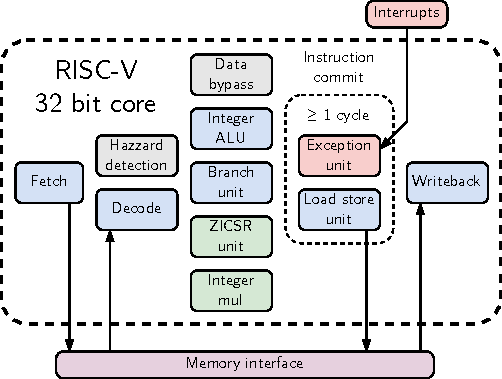
\includegraphics[width=0.8\textwidth]{root/Imagenes/estado_del_arte/riscv_core.pdf}
	\caption{Ruta de datos del procesador RISC-V utilizado. Los bloques relacionados con la arquitectura base RV32I se muestran en azul, los bloques para detectar riesgos de datos en gris, los bloques relacionados con el modo M en rojo, los bloques de extensiones estándar extra en verde y en morado el interfaz con el bus de memoria.}
	\label{fig:riscv_data_pipeline}
\end{figure}

\section{Redes Neuronales Bayesianas}

El aprendizaje automático es una rama de la inteligencia artificial que se centra en el desarrollo de algoritmos y modelos estadísticos que permiten generalizar respuestas en problemas para los que no han sido explícitamente programados aprendiendo de un conjunto de datos dado.

Las NN son modelos de aprendizaje automático cuya estructura está inspirada en el funcionamiento de redes de neuronas biológicas \cite{deep_learning_nature}. Una NN está compuesta por capas de neuronas conectadas entre sí. Cada capa cuenta con un conjunto de pesos y una función de activación. Las NN necesitan un proceso de entrenamiento en el que son expuestas a un conjunto de datos etiquetados para que puedan ajustar el valor de los pesos de las diferentes capas. En los últimos años, las NN han obtenido muy buenos resultados en problemas de clasificación y regresión entre otros \cite{cnn_image_survey}.

Las BNN son un tipo de NN que integran modelado probabilístico, lo que les permite cuantificar la incertidumbre en tareas de aprendizaje automático, mejorando su confianza y fiabilidad \cite{bnn_hyper_uncertainty}. Sin embargo, necesitan más parámetros para definir los pesos, normalmente el doble que una NN convencional, y la inferencia es más compleja. Los pesos de las BNN son distribuciones de probabilidad, normalmente distribuciones gaussianas, que se han de muestrear durante las propagaciones de la entrada. El algoritmo de inferencia más común para las BNN requiere múltiples propagaciones de la entrada de la red, aumentando drásticamente el coste computacional del mismo \cite{bnn_theory_paper}.

La Figura \ref{fig:bnn_vs_nn_example} muestra la utilidad de las métricas de incertidumbre con un ejemplo simple. Considerando una NN convencional y una BNN ambas entrenadas para clasificar imágenes de perros y gatos, en el caso de que se les pidiera clasificar un dato anómalo, como la imagen de un tigre, con la BNN se obtendría un valor de incertidumbre alto, indicando una anomalía en la predicción, mientras que con una NN convencional no se tendría ningún indicio de que el dato de entrada era anómalo.

\begin{figure}[h]
	\centering
	\includegraphics[width=\textwidth]{root/Imagenes/estado_del_arte/nn_bnn_example.pdf}
	\caption{Ejemplo sencillo de utilidad de las métricas de incertidumbre aportadas por las BNN. Una NN convencional y una BNN, ambas entrenadas para clasificar imágenes de perros y gatos, reciben como entrada la imagen de un tigre. La BNN es capaz de detectar el dato anómalo mientras que la NN convencional no.}
	\label{fig:bnn_vs_nn_example}
\end{figure}

La Figura \ref{fig:neuron_comparation} muestra una comparación sencilla de una neurona clásica y de una neurona bayesiana, ambas con una función de activación de rectificación (\textit{\textbf{Re}ctified \textbf{L}inear \textbf{U}nit}).

% Vertically alling two sufigures and keep subcaption using floatrow and subcaptions pkgs
\begin{figure}[htb]
  \floatsetup{heightadjust=all, valign=c}
  \begin{subcaptiongroup}
  \begin{floatrow}
	\ffigbox{%
  	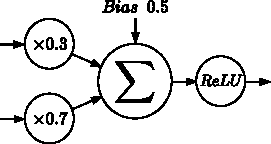
\includegraphics[width=0.48\textwidth]{root/Imagenes/estado_del_arte/clasic_neuron.pdf}
	}{%
  	\caption{Neurona clásica}%
  	\label{fig:clasic_neuron}%
	}
	\ffigbox{%
  	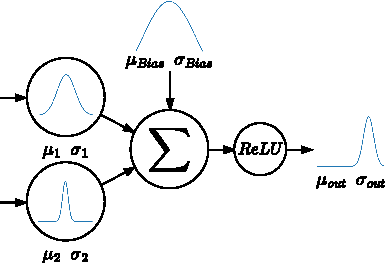
\includegraphics[width=0.49\textwidth]{root/Imagenes/estado_del_arte/bnn_neuron.pdf}
	}{%
  	\caption{Neurona bayesiana}%
  	\label{fig:bnn_neuron}%
	}
  \end{floatrow}
  \end{subcaptiongroup}
  \caption{Comparación de una neurona clásica con respecto a una neurona bayesiana, ambas con la misma función de activación ReLU. Los pesos de la neurona convencional son valores estáticos mientras que los de la neurona bayesiana son distribuciones gaussianas parametrizadas mediante medias y desviaciones típicas.}%
  \label{fig:neuron_comparation}%
\end{figure}

En un entorno IoT donde los datos pueden ser incompletos o ruidosos la capacidad de cuantificar la incertidumbre es crucial para tomar decisiones confiables en aplicaciones críticas. Por lo que las BNN son una muy buena herramienta para mejorar la precisión y la robustez de los sistemas de aprendizaje automático en estos entornos.

Las métricas de incertidumbre proporcionadas por las BNN son muy útiles para detectar diferentes tipos de situaciones. Por ejemplo, pueden servir para valorar la confianza de la predicción, si una predicción tiene una alta incertidumbre podría indicar que es menos confiable y que requeriría de verificación humana. También pueden utilizarse para valorar la calidad los datos de entrenamiento, si los datos de entrenamiento contienen muestras mal etiquetadas sus predicciones tendrán una mayor incertidumbre asociada. Alcolea \emph{et al.} \cite{bnn_hyper_uncertainty} mostraron que existe una clara correlación entre la incertidumbre y la precisión en un modelo bien entrenado, por tanto la incertidumbre se puede utilizar para identificar salidas con menor probabilidad de acierto de la requerida. También observaron que al entrenar una BNN con los datos de 2 clases mezclados se aprecia un claro incremento en la incertidumbre de las predicciones asociadas a esas clases, y que la incertidumbre aumentaba cuando se añadía ruido aleatorio a las entradas. Otro posible uso es detectar que los datos de entrenamiento no reflejan correctamente la realidad, predicciones con alta incertidumbre pueden indicar que los datos que está procesando el modelo no se parecen a los datos con los que ha sido entrenado. En entornos dinámicos como IoT, donde las condiciones pueden cambiar rápidamente, si la incertidumbre en las predicciones aumenta repentinamente, puede indicar un cambio en el entorno que requiera una recalibración del modelo.

\subsection{Fundamentos teóricos} \label{sec:bnn_formulas}

Estas redes neuronales se basan el Teorema de Bayes,  mostrado en la Ecuación \ref{eq:bayes_theo}, para modelar la probabilidad de un conjunto de pesos $w$ dado un conjunto de datos de entrenamiento $D = \{x, y\}$. Esta distribución de probabilidad es la probabilidad a posteriori.
\begin{equation} \label{eq:bayes_theo}
p(w|D) = \dfrac{p(D|w) p(w)}{p(D)}
\end{equation}

El entrenamiento de una BNN consiste en calcular esta distribución a posteriori. Calcular esta distribución para un modelo grande y complicado como una BNN es intratable. Para aproximar esta distribución se utilizan métodos de inferencia bayesiana. El método más común es la inferencia variacional, que aproxima la distribución a posteriori usando una más simple $q_{\phi}(w)$. Esta aproximación se realiza minimizando la divergencia de Kullback-Leibler \cite{kl_divergence} entre $q_{\phi}(w)$ y $p(w|D)$ mediante la actualización de un conjunto de parámetros $\phi$. Teóricamente, las distribuciones podrían tener cualquier forma, pero para reducir el espacio de búsqueda sólo se utilizan distribuciones simétricas y simples. Las distribuciones gaussianas son una buena opción porque solo se definen con dos parámetros, lo que ayuda a reducir el tamaño del modelo.

En consecuencia, una BNN entrenada consiste en un conjunto de medias y desviaciones de diferentes distribuciones gaussianas $\phi = \{\mu, \sigma\}$, lo que significa que los pesos se convierten en distribuciones de probabilidad en lugar de valores fijos, y la salida también se convierte en una distribución en lugar de un valor único. Esto permite medir la incertidumbre de la predicción. La Ecuación \ref{eq:bayes_inference} muestra la distribución de predicción a posteriori de una nueva observación $x^*$.
\begin{equation} \label{eq:bayes_inference}
p(y^*|x^*,D) = \int p(y|x^*,w) p(w|D) dw
\end{equation}

Mediante métodos de Monte Carlo se puede aproximar la integral de la Ecuación \ref{eq:bayes_inference}. En este caso, las muestras son diferentes propagaciones estocásticas de la entrada. En cada una de estas propagaciones, los pesos se muestrean de las distribuciones gaussianas que forman la distribución a posteriori aproximada.

Siendo $T$ el número de muestras, $K$ el número de clases posibles y una muestra $a_t$ el vector de longitud $K$ de componentes $p(y^* = c_k | x^*, w_t)$. Cada uno de sus componentes representa la probabilidad de que $y^*$ sea $c_k$. Para obtener una única predicción se puede tomar el componente máximo del vector promedio de todas las muestras.

\subsubsection{Cálculo de la incertidumbre}

En problemas de clasificación, se puede medir la incertidumbre de una predicción utilizando las diferentes muestras Monte Carlo obtenidas \cite{uncertainty_metrics}. A continuación se explica como obtener las métricas más relevantes y lo que representan.

La incertidumbre predictiva ($\mathbb{H}$) representa la incertidumbre de una predicción en el rango $[0, \log(K)]$ y puede calcularse utilizando la Ecuación \ref{eq:predictive_uncertainty}.
\begin{equation} \label{eq:predictive_uncertainty}
\mathbb{H}(y|x,D) = - \sum^K_{k=1} \left[ \left( \dfrac{1}{T} \sum^T_{t=1} a_t \right) \log\left( \dfrac{1}{T} \sum^T_{t=1} a_t \right) \right]
\end{equation}

La incertidumbre puede dividirse en dos, aleatoria y epistémica, $\mathbb{H}$ captura ambas. La entropía esperada ($\mathbb{E}p$) captura la incertidumbre aleatoria, que es causada por ambigüedades en el conjunto de datos como mediciones ruidosas, clases superpuestas o muestras mal etiquetadas. $\mathbb{E}p$ puede calcularse utilizando la Ecuación \ref{eq:expected_entropy}.
\begin{equation} \label{eq:expected_entropy}
\mathbb{E}{p(w|D)}[\mathbb{H}(y|x,D)] = \dfrac{1}{T} \sum^T{t=1} \left( -\sum^K_{k=1} a_{t} \log(a_t) \right)
\end{equation}

La incertidumbre epistémica representa lo que el modelo no sabe debido a la falta de datos durante el proceso de entrenamiento, y puede calcularse utilizando la información mutua (\textit{\textbf{M}utual \textbf{I}nformation}) mostrada en la Ecuación \ref{eq:mutual_information}.
\begin{equation} \label{eq:mutual_information}
MI(y,w|x,D) = \mathbb{H}(y|x,D) - \mathbb{E}_{p(w|D)}[\mathbb{H}(y|x,D)]
\end{equation}

\subsection{Aceleración hardware}

La aceleración de algoritmos de aprendizaje automático es un campo de investigación muy activo con muchas propuestas recientes \cite{survey_ai22}. La aceleración de las BNN no es una excepción, debido en parte al elevado coste de su algoritmo de inferencia. Otros trabajos se han centrado en desarrollar aceleradores de alto rendimiento para el proceso completo de inferencia \cite{bnn_grng_accel, sampling_free_bnn_accel, bnn_clt_approx}.

Awano \emph{et al.} propusieron un acelerador sin múltiples propagaciones ni muestreo para el algoritmo de inferencia de las BNN, reemplazando la función de activación ReLU por una función cuadrática \cite{sampling_free_bnn_accel}. Su trabajo muestra buenos resultados para el conjunto de datos MNIST, pero otros trabajos han demostrado que este enfoque no es generalizable y no funciona bien con otros modelos \cite{bnn_clt_approx}. Por esta razón, este trabajo se centra en el algoritmo de múltiples propagaciones con muestreo, ya que es el método más estándar y ha sido ampliamente demostrado que da buenos resultados para varios diferentes conjuntos de datos \cite{bnn_grng_accel, bnn_clt_approx, bnn_hyper_uncertainty}.

El muestreo de distribuciones para generar los pesos es una parte fundamental de los trabajos que siguen el enfoque de múltiples propagaciones. Cai \emph{et al.} propusieron un acelerador de inferencia de BNN con 2 posibles GRNG \cite{bnn_grng_accel}. Uno basado en el teorema central del límite (TCL) utilizando la distribución binomial y otro en el método de Wallace \cite{wallace_grng}.

Los GRNG son un tema que ya ha sido explorado en profundidad \cite{grng_survey}. Trabajos anteriores han mostrado que los GRNG basados en el CLT no muestran una precisión elevada en la cola de la distribución \cite{clt_grng}. Sin embargo, en el caso de la inferencia de las BNN no es necesario tener un GNRG preciso. Hirayama \emph{et al.} demostraron que utilizando un GRNG de poca precisión basado en una \textit{Lookup Table} (LUT) se obtienen buenos resultados \cite{bnn_lut_grng}.

En otro trabajo Awano \emph{et al.} diseñaron un acelerador que aproximan la salida final del modelo utilizando generadores hardware de muestras Bernoulli, bajo la condición de que el TCL podría aplicarse al modelo en general \cite{bnn_clt_approx}. La Figura \ref{fig:b2n2_clt} muestra un diagrama de su aproximación.

\begin{figure}[h]
	\centering
	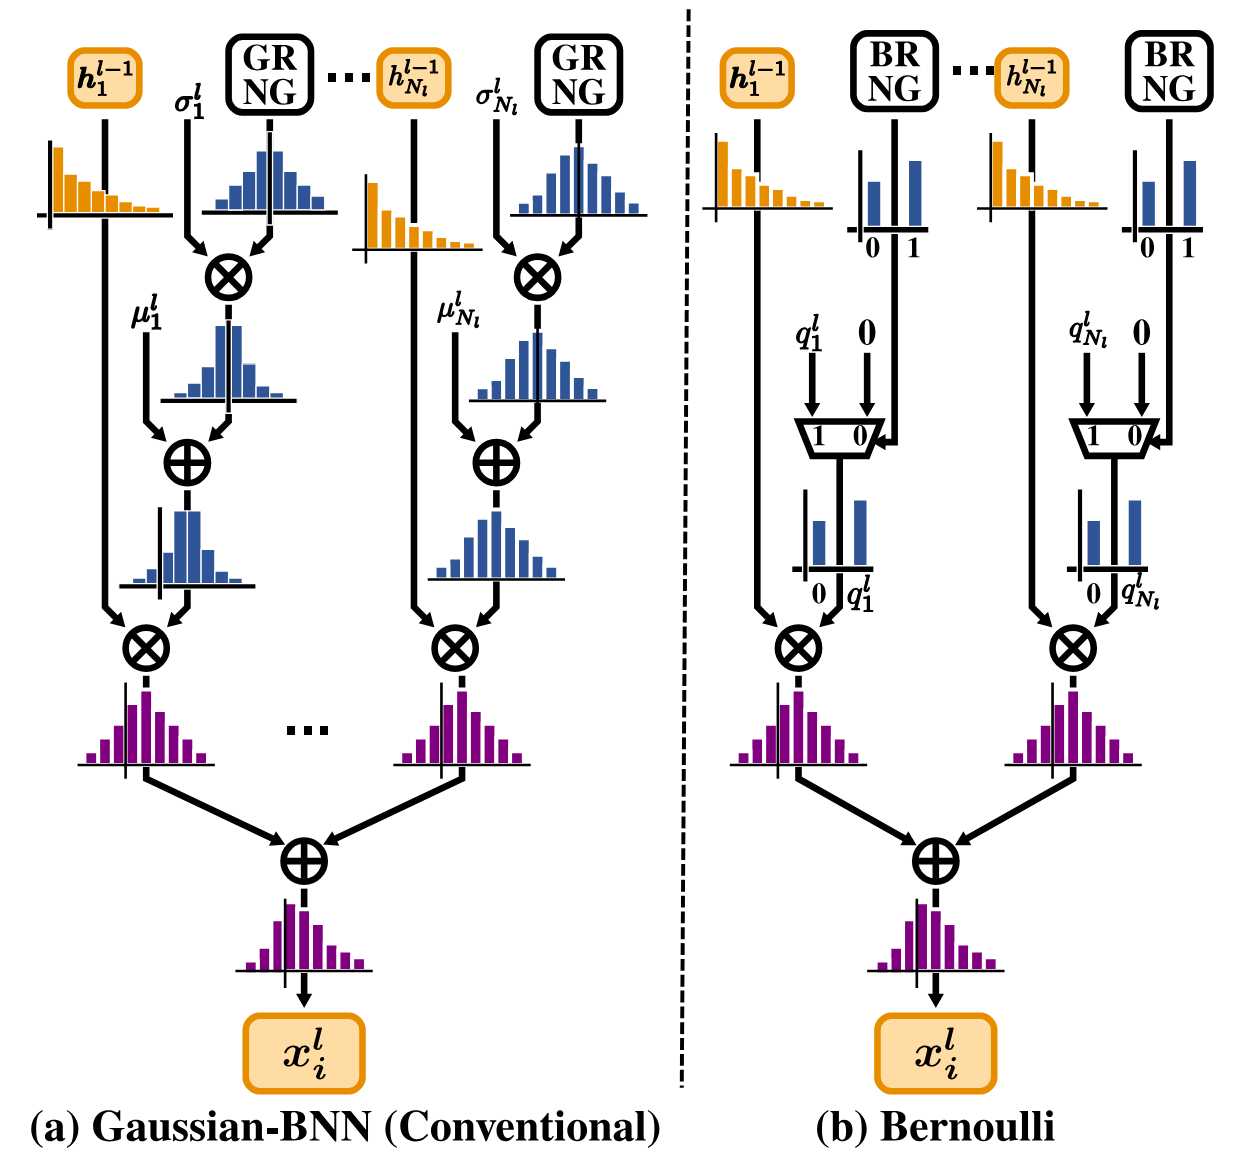
\includegraphics[width=0.55\textwidth]{root/Imagenes/estado_del_arte/b2n2_clt.png}
	\caption{Comparación de muestrear distribuciones gaussianas o distribuciones de Bernoulli en una BNN. Debido al TCL la distribución final es independiente de las distribuciones muestreadas \cite{bnn_clt_approx}.}
	\label{fig:b2n2_clt}
\end{figure}

Una ventaja clave de los generadores de muestras Bernoulli radica en su implementación en hardware. A diferencia de los métodos de software que dependen de operaciones de salto, que pueden degradar el rendimiento de las CPU modernas, los generadores hardware pueden implementarse utilizando componentes simples como comparadores y multiplexores, lo que los hace de bajo coste y eficientes.

\subsection{Soporte de bibliotecas}

Este trabajo tiene como objetivo ejecutar inferencia de estas redes en entornos RISC-V de bajas prestaciones, donde actualmente no existe un conjunto de bibliotecas que lo permita. TensorFlow Probability permite entrenar y ejecutar inferencia de BNN utilizando precisión en punto flotante. Por otro lado, en el caso de PyTorch, existe BayesianTorch desarrollado por IntelLabs, que ofrece la misma funcionalidad \cite{bayesian_torch}.

TensorFlowLite  es la versión de TensorFlow diseñada para sistemas empotrados, ofrece funcionalidades como la cuantización de modelos y la inferencia utilizando precisión de enteros para las NN convencionales, sin embargo, aún no tiene soporte para BNN \cite{tflite}. En una actualización reciente, BayesianTorch ha añadido soporte para la cuantización de BNN \cite{bnn_quant}. Este trabajo se centra en el ecosistema de Tensorflow debido a que se han utilizado modelos desarrollados en dicho entorno para su validación.

\chapter{Metodología}

\section{Herramientas utilizados}

El diseño del procesador base utilizado se encuentra en el repositorio riscv-vhdl \cite{base_riscv_cpu_git}. Para definir la extensión del procesador RISC-V se ha utilizado el lenguaje de especificación hardware VHDL. Para simular el comportamiento del procesador se ha utilizado el simulador GHDL \cite{ghdl} junto con el visor de ondas GTKWave \cite{gtkwave}. Los programas que se han ejecutado en los procesadores simulados se han desarrollado en C y para compilarlos se ha utilizado el conjunto de herramientas GNU RISC-V Compiler Toolchain \cite{gcc_riscv}. 

Para entrenar BNNs se ha utilizado la biblioteca de Python TensorFlow Probability \cite{tfprob} junto al repositorio BNN\_for\_hyperspectral\_datasets\_analysis \cite{bnn_hyper_git}. El proceso de compilación y pruebas se han automatizado todo lo posible mediante la herramienta Make y \textit{scripts} en Bash y Python. Para manejar ficheros ELF desde Python se ha utilizado la biblioteca pyelftools \cite{pyelftools}. Para crear gráficas se ha utilizado la biblioteca de Python Matplotlib \cite{matplotlib}. Se han utilizado los test estadísticos de la biblioteca de Python SciPy \cite{scipy}.

Se ha utilizado la plataforma de desarrollo Xilinx ZCU104 FPGA \cite{fpga_board} junto a Vivado Design Suite \cite{vivado} para implementar los diseños hardware sobre una FPGA y analizar sus costes.

Para redactar este documento se ha utilizado el editor de \LaTeX\ en línea Overleaf \cite{overleaf} y para crear los diagramas se utilizado el editor en línea draw.io \cite{drawio} junto al editor de gráficos vectoriales Inkscape \cite{inkscape}.

Como programa de control de versiones se ha utilizado Git \cite{git} junto con GitHub \cite{github} como repositorio en línea.

\section{Modelos utilizados}

Durante el proceso de verificación se han utilizado tres arquitecturas de modelos diferentes. La Tabla \ref{tab:hyper_models} muestra la arquitectura de los modelos para clasificación de píxeles hiperespectrales \cite{bnn_hyper_uncertainty}. Los conjuntos de datos utilizados para este modelo son diferentes imágenes hiperespectrales obtenidas mediante satélite denominadas BO, IP, KSC, PU y SV.

%%%%

\begin{table}[h]
    \centering
    \caption{Arquitectura de los modelos para clasificación de píxeles hiperespectrales.}
    \label{tab:hyper_models}
    \begin{tabular}{lll}
    \hline
         \textbf{Layer Type} & \textbf{Input} & \textbf{Output}\\ \hline
         Dense & Number of spectral bands & 32\\
         Dense & 32 & 16\\
         Dense & 16 & Number of pixel classes\\ \hline
    \end{tabular}
\end{table}

La Tabla \ref{tab:cnn_models} muestra una arquitectura LeNet-5 bayesiana. LeNet-5 es una arquitectura de red neuronal convolucional (\textit{\textbf{C}onvolutional \textbf{N}eural \textbf{N}etwork}) simple \cite{lenet}. Se ha entrenado un modelo con la misma arquitectura para reconocer el conjunto de datos MNIST \cite{MNIST_dataset} y CIFAR-10 \cite{CIFAR_dataset} pero utilizando capas bayesianas.

\begin{table}[h]
    \centering
    \caption{Arquitectura LeNet-5 bayesiana.}
    \label{tab:cnn_models}
    \begin{tabular}{llll}
        \hline
         \textbf{Layer Type} &  \textbf{Input} &  \textbf{Output} & \textbf{Kernel Size} \\ \hline
         Conv2D Valid & 28$\times$28 & 24$\times$24$\times$6 & 5$\times$5 \\
         MaxPool2D & 24$\times$24$\times$6 & 12$\times$12$\times$6 & 2$\times$2 \\
         Conv2D Valid & 12$\times$12$\times$6 & 8$\times$8$\times$16 & 5$\times$5 \\
         MaxPool2D & 8$\times$8$\times$16 & 4$\times$4$\times$16 & 2$\times$2 \\
         Conv2D Valid & 4$\times$4$\times$16 & 1$\times$1$\times$120 & 4$\times$4 \\
         Dense & 120 & 84 & \\
         Dense & 84 & 10 & \\ \hline
    \end{tabular}
\end{table}

La Tabla \ref{tab:b2n2_model} muestra la arquitectura B2N2, propuesta por Awano \emph{et al.} junto a su acelerador para BNN \cite{bnn_clt_approx}. También se ha entrenado para reconocer los conjuntos de datos MNIST y CIFAR-10.

\begin{table}[h]
    \centering
    \caption{Arquitectura B2N2.}
    \label{tab:b2n2_model}
    \begin{tabular}{llll}
    \hline
    \textbf{Layer Type} & \textbf{Input} & \textbf{Output} & \textbf{Kernel Size}\\ \hline
    Conv2D Same & 32$\times$32 & 32$\times$32$\times$32 & 3$\times$3 \\
    Conv2D Same & 32$\times$32$\times$32 & 32$\times$32$\times$32 & 3$\times$3 \\
    MaxPool2D & 32$\times$32$\times$32 & 16$\times$16$\times$32 & 2$\times$2 \\
    Conv2D Same & 16$\times$16$\times$32 & 16$\times$16$\times$64 & 3$\times$3 \\
    Conv2D Same & 16$\times$16$\times$64 & 16$\times$16$\times$64 & 3$\times$3 \\
    MaxPool2D & 16$\times$16$\times$64 & 8$\times$8$\times$64 & 2$\times$2 \\
    Conv2D Same & 8$\times$8$\times$64 & 8$\times$8$\times$128 & 3$\times$3 \\
    Conv2D Same & 8$\times$8$\times$128 & 8$\times$8$\times$128 & 3$\times$3 \\
    MaxPool2D & 8$\times$8$\times$128 & 4$\times$4$\times$128 & 2$\times$2 \\
    Dense & 2028 & 10 & \\ \hline
    \end{tabular}
\end{table}


\section{Configuración experimental}

La Figura \ref{fig:experiment_pipeline} muestra el proceso y componentes para ejecutar inferencia de BNN de manera eficiente en un procesador RISC-V con soporte único para precisión entera que se han utilizado para obtener los resultados de este trabajo.

\begin{figure}[h]
    \centering
    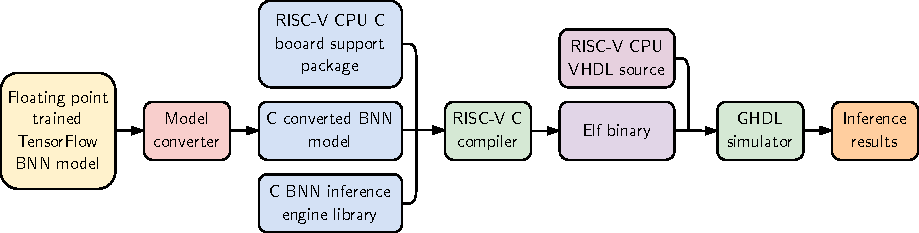
\includegraphics[width=\textwidth]{root/Imagenes/4_bnn_riscv/experiment_pipeline.pdf}
    \caption{Diagrama de componentes necesarios para ejecutar la inferencia de BNN en un procesador RISC-V simulado. Los componentes marcados con un número son contribuciones de este trabajo.}
    \label{fig:experiment_pipeline}
\end{figure}

\subsection{Conversor de modelos}

Se ha desarrollado una herramienta en Python que convierte modelos BNN TensorFlow ya entrenados en precisión de punto flotante a ficheros de código C con precisión en coma fija, marcado en la Figura \ref{fig:experiment_pipeline} como componente 1, que puedan ejecutarse junto al motor de inferencia explicado en el Capítulo \ref{ch:motor_inferencia}. La Figura \ref{fig:model_converter} muestra un diagrama de las diferentes operaciones que realiza esta herramienta.

\begin{figure}[h]
    \centering
    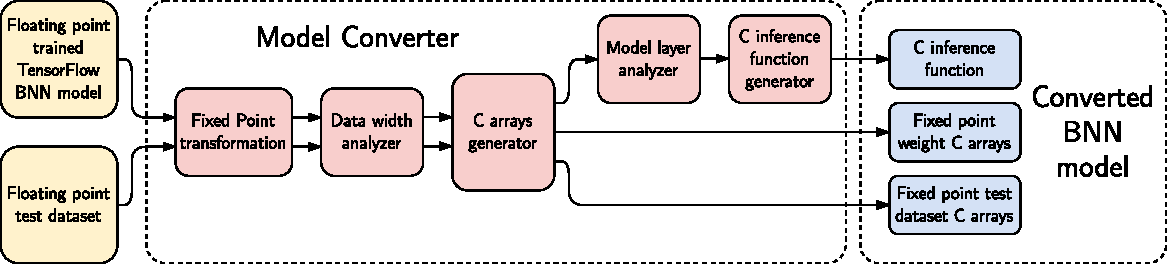
\includegraphics[width=\textwidth]{root/Imagenes/metodologia/model_converter.pdf}
    \caption{Diagrama de componentes internos del conversor de modelos.}
    \label{fig:model_converter}
\end{figure}

\subsubsection{Precisión en coma fija}

Implementar aritmética de coma flotante en hardware es caro, por lo que es común que procesadores de bajas prestaciones no dispongan de dicho hardware. GCC permite emular las operaciones de coma flotante mediante software, comúnmente conocido como \textit{soft-float}. Esta emulación tiene un gran impacto en el rendimiento por lo que no se ha utilizado.

Con el objetivo de obtener un mejor rendimiento se ha utilizado el formato coma fija para representar los números decimales. Este formato permite representar números decimales y operar con ellos utilizando hardware de precisión entera, lo que tiene un impacto muy pequeño en el rendimiento. Esta codificación consiste en multiplicar los números con una escala potencia de 2. A mayor sea la escala mayor precisión se obtiene. La principal limitación de esta codificación es el tamaño de palabra de la arquitectura ya que pueden ocurrir desbordamientos al operar con números multiplicados por una escala grande. Por lo que en general se obtiene menor precisión que con la codificación en punto flotante. La Figura \ref{fig:fixed_point} muestra un ejemplo de este tipo de codificación.

\begin{figure}[h]
    \centering
    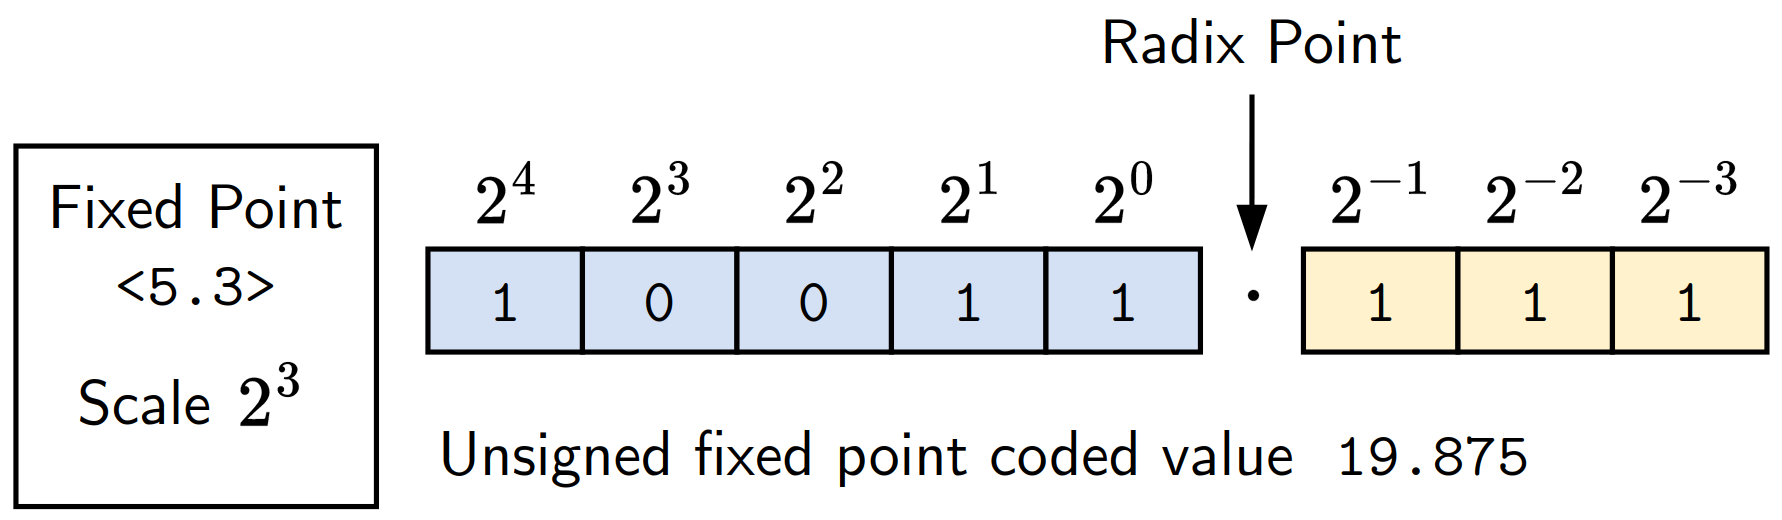
\includegraphics[width=0.7\textwidth]{root/Imagenes/metodologia/fixed_point.png}
    \caption{Ejemplo de codificación en coma fija sin signo \texttt{<5.3>} del valor 19.875.}
    \label{fig:fixed_point}
\end{figure}

\subsection{Actualización del Board Support Package}

El \textit{\textbf{B}oard \textbf{S}upport \textbf{P}ackage} (BSP) de una plataforma es una capa de software intermedia entre la aplicación y el hardware que contiene código especifico para crear un entorno de ejecución estable en dicha plataforma. Además puede proveer de los ficheros de configuración y un sistema de compilación. En la Figura \ref{fig:experiment_pipeline} aparece componente 2. En la Figura \ref{fig:bsp} se muestra un diagrama con mas detalle sobre este componente.

\begin{figure}[h]
    \centering
    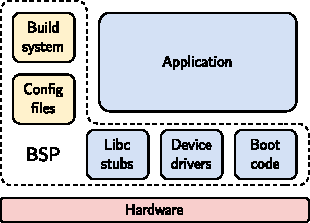
\includegraphics[width=0.6\textwidth]{root/Imagenes/metodologia/bsp.pdf}
    \caption{Diagrama de componentes que forman un BSP y como se sitúa entre la aplicación y el hardware.}
    \label{fig:bsp}
\end{figure}

Con el objetivo de mejorar la experiencia de desarrollo del motor de inferencia se actualizó el BSP del procesador para dar soporte a la biblioteca estándar C (libc) y algunas funcionalidades de C++. De esta forma se pueden utilizar funciones útiles de libc cómo \texttt{printf}, o \texttt{memset} entre otras. Para ello se actualizaron las herramientas y ficheros de compilación, se añadieron funciones \textit{stub} para las llamadas al sistema no implementadas y se implementaron versiones modificadas de \texttt{\_write} y \texttt{\_exit}.


\subsection{Verificación}

Para analizar el correcto funcionamiento del motor de inferencia y estudiar el impacto en el rendimiento de las optimizaciones posteriores se ha desarrollado una herramienta que compara las predicciones del conjunto de datos de prueba obtenidas con el motor de inferencia y TensorFlow de forma automática. Este componente aparece en la Figura \ref{fig:experiment_pipeline} como componente 6.

Para comparar los conjuntos de predicciones se han utilizado las métricas de incertidumbre y la precisión. La precisión se puede calcular como el ratio de predicciones acertadas sobre el número total de predicciones. Analizar las métricas de incertidumbre y las propiedades estadísticas de los modelos es complejo. Para hacerlo se han utilizado 4 tipos de gráficas que las representan, estas se explicaran mas adelante en la Sección \ref{sec:uncertainty_example} mediante ejemplos.


\chapter{Motor de inferencia para Redes Neuronales Bayesianas} \label{ch:motor_inferencia}

\section{Biblioteca desarrollada en C}

Se ha desarrollado una biblioteca de funciones que ejecutan la inferencia de capas BNN estándar y convolucionales con funciones de activación ReLU o exponenciales normalizadas (SoftMax) utilizando precisión de coma fija, ya que los paquetes standard como TensorFlow o pytorch no ofrecen esta funcionalidad para dispositivos IoT. Esta biblioteca se ha desarrollado en C y se muestra en la Figura \ref{fig:experiment_pipeline} como el componente número 3.

\subsection{Aproximación de la función logaritmo}

Para calcular las métricas de incertidumbre se necesita la función logaritmo por lo que se ha implementado una versión del algoritmo desarrollado por Turner para calcular el logaritmo de un número en coma fija~\cite{binary_log}.

\subsection{Aproximación de la función SoftMax}

Mientras que calcular la función ReLU es trivial la función SoftMax no, por lo que una de las contribuciones de este trabajo ha sido crear una aproximación de esta función, explicada a continuación. La función toma un vector de componentes $x \in X$ de tamaño $N$ como entrada y devuelve otro del mismo tamaño cuyos componentes $y\in Y$ se calculan según la Ecuación \ref{eq:softmax}.
\begin{equation} \label{eq:softmax}
y_i = \dfrac{e^{x_i}}{\sum_{j = 0}^N e^{x_j}}
\end{equation}

Para calcular esta función utilizando coma fija es necesario calcular la función exponencial en dicho formato. Para evitar desbordamientos de la función exponencial se va a utilizar la función SoftMax equivalente mostrada en la Ecuación \ref{eq:softmax_neg}.
\begin{equation} \label{eq:softmax_neg}
y_i = \dfrac{e^{x_i - \max(X)}}{\sum_{j = 0}^N e^{x_j - \max(X)}}
\end{equation}

En esta versión de la función se cumple que $x_i \in (-\infty, 0]$ por lo que $e^{x_i} \in (0,1]$. Para calcular la función exponencial se va a utilizar la Ecuación \ref{eq:split_exp}, dividiendo la entrada $x_i$ en su parte entera $a_i$ y su parte decimal $b_i$.
\begin{equation} \label{eq:split_exp}
e^{x_i} = e^{a_i+b_i} = e^{a_i} e^{b_i}
\end{equation}

La parte entera $e^{a_i}$ se calcula mediante una LUT de 20 entradas para el rango $[e^{-19}, e^{0}]$. A partir de $e^{-19}$ los valores son demasiado pequeños como para representarlos con la precisión disponible por lo que siempre valen $0$. La parte decimal $e^{b_i}$ se aproxima mediante los 8 primeros términos de la serie de Taylor mostrada en la Ecuación \ref{eq:exp_taylor}. Para optimizar y evitar las divisiones los valores de $\dfrac{1}{n!}$ para $n \in [2,7]$ se han almacenado en una LUT.
\begin{equation} \label{eq:exp_taylor}
e^{b_i} \approx \sum_{n=0}^{7} \dfrac{{b_i}^n}{n!}
\end{equation}

La Figura \ref{fig:exp_aprox} muestra un estudio de la precisión de la aproximación. Se comparan sus resultados con los de la implementación de la función exponencial de la biblioteca estándar en punto flotante. Como medida cuantitativa del error se ha utilizado el error cuadrático medio (\textit{\textbf{M}ean \textbf{S}quared \textbf{E}rror}). Se aprecia cómo se obtiene una buena aproximación en el rango deseado.

\begin{figure}[h]
	\centering
	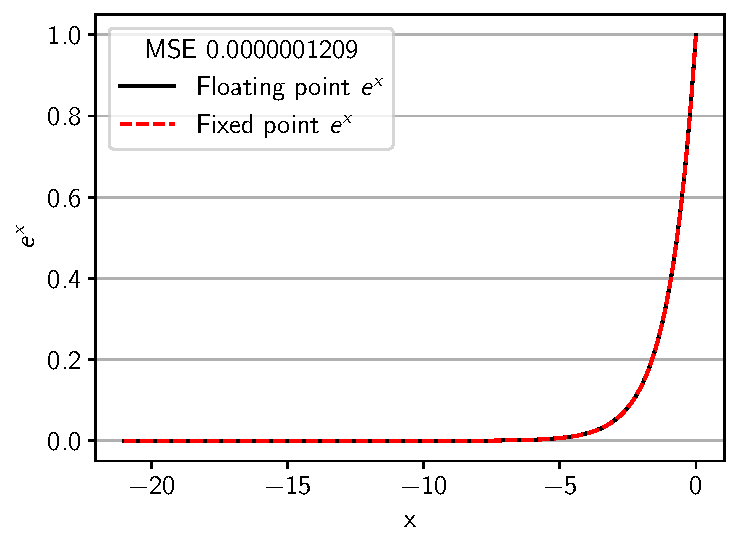
\includegraphics[width=0.55\linewidth]{root/Imagenes/bnn_lib/exp_aprox.pdf}
	\caption{Comparación de la función $e^x$ de la biblioteca estándar en punto flotante (línea negra) con la aproximación en coma fija implementada (línea roja discontinua) en el rango $[-20,0]$.}
	\label{fig:exp_aprox}
\end{figure}

\subsection{Muestreo de distribuciones Gaussianas}

Como se ha explicado previamente, las BNN necesitan muestrear distribuciones gaussianas. Como método de muestreo base se ha utilizado un algoritmo basado en la suma de distribuciones uniformes, dicha suma se aproxima a una distribución gaussiana debido al TCL, como se muestra en la Ecuación \ref{eq:tcl_unif}.
\begin{equation} \label{eq:tcl_unif}
\sum_{n=0}^{N} \mathcal{U}_n(0,1) \sim \mathcal{N} \left( \dfrac{N}{2}, \sqrt{\dfrac{N}{12}} \right)
\end{equation}

El algoritmo implementado genera muestras de $\mathcal{N}(0,1)$ para luego transformarlas en muestras de una distribución gaussiana arbitraria $\mathcal{N}(\mu, \sigma)$ de media $\mu$ y desviación típica $\sigma$ utilizando la Ecuación \ref{eq:gauss_linear}.
\begin{equation} \label{eq:gauss_linear}
\mathcal{N}(\mu, \sigma) = \sigma \mathcal{N}(0,1) + \mu
\end{equation}

La aproximación empleada utiliza la suma de 12 distribuciones uniformes y posteriormente centra la distribución como muestra la Ecuación \ref{eq:tcl_12center}.
\begin{equation} \label{eq:tcl_12center}
\sum_{n=0}^{12} \mathcal{U}_n(0,1) - 6 \sim \mathcal{N}(0,1)
\end{equation}

La Figura \ref{fig:gauss_aprox} muestra un análisis estadístico del método de muestreo implementado. En el gráfico Q-Q se aprecia como los cuantiles del conjunto de muestras son muy parecidos a los cuantiles teóricos, mostrando desviaciones en las colas como es de esperar de esta aproximación. En el histograma se aprecia como las muestras se ajustan bastante bien a la distribución teórica.

\begin{figure}[h]
	\centering
	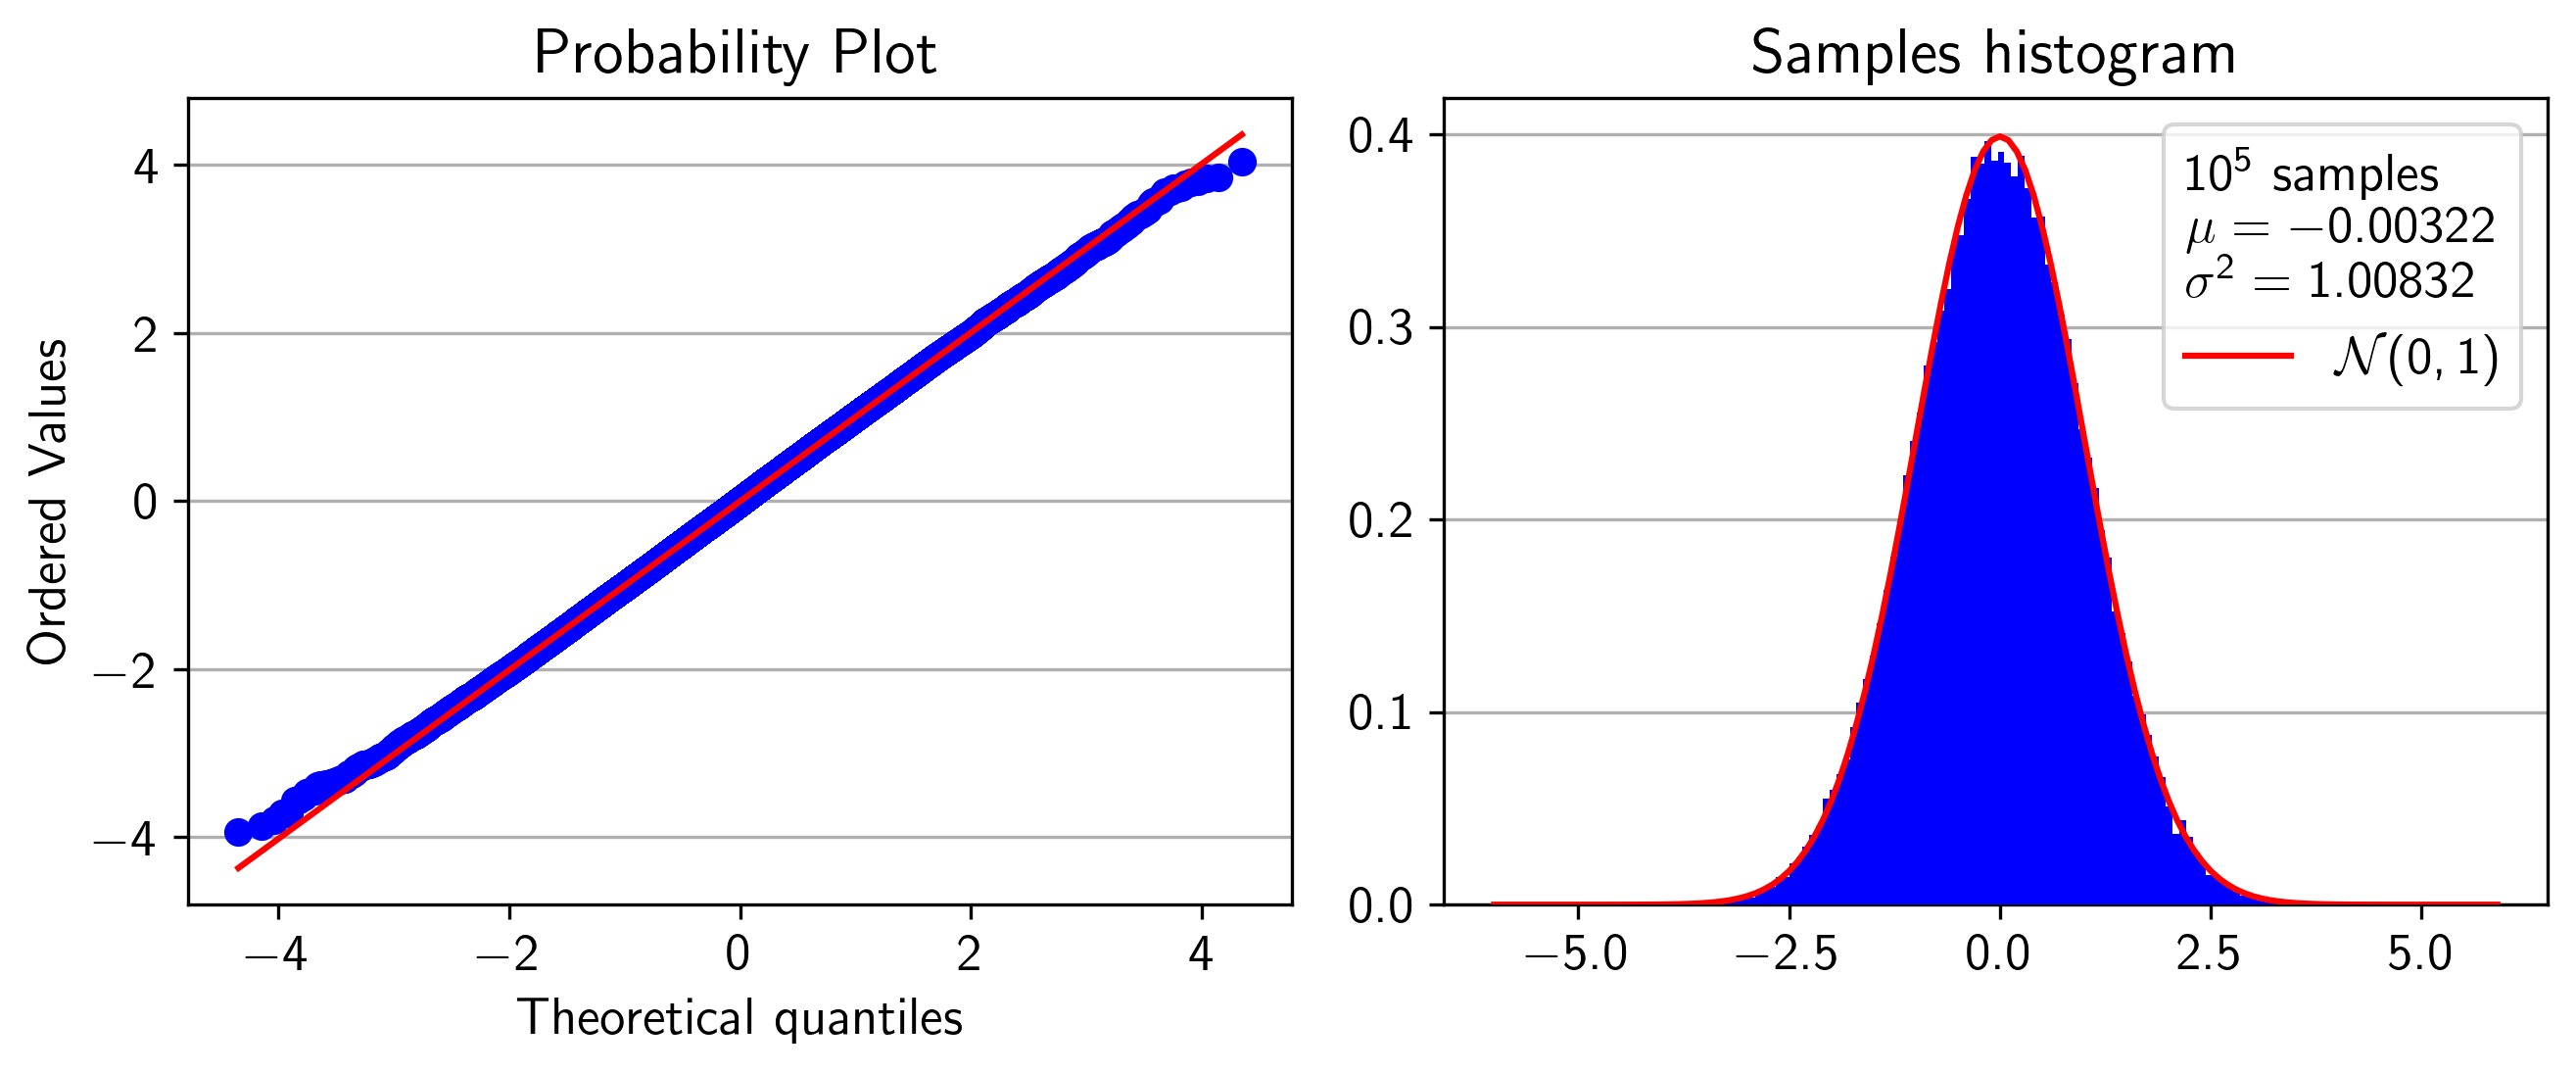
\includegraphics[width=\textwidth]{root/Imagenes/bnn_lib/gaus_aprox.png}
	\caption{Análisis estadístico de $10^5$ muestras del GRNG implementado (azul) con respecto a $\mathcal{N}(0,1)$ (rojo). A la izquierda se muestra un gráfico Q-Q. A la derecha se muestra un histograma.}
	\label{fig:gauss_aprox}
\end{figure}

Además de las gráficas mostradas también se han utilizado los test de bondad de ajuste de D’Agostino \emph{et. al.} \cite{normaltest_1, normaltest_2} y el de Kolmogorov-Smirnov \cite{kstest}.

\subsection{Muestreo de distribuciones Uniformes}

Generar muestras de distribuciones uniformes es una parte del algoritmo para generar muestras de una distribución gaussiana explicado previamente. Para hacerlo se utiliza una versión del algoritmo Xorshift de 32 bits \cite{xorshift}. Es un algoritmo sencillo para generar números pseudoaleatorios solamente con instrucciones \texttt{xor} y \texttt{shift}.

\section{Análisis de resultados} \label{sec:uncertainty_example}

La Figura \ref{fig:figure_example} muestra un ejemplo de las gráficas utilizadas para validar las métricas de incertidumbre y propiedades estadísticas. Estas gráficas se han creado utilizando las predicciones para el conjunto de datos de píxeles hiperespectrales KSC. \ref{fig:example_hist} muestra un histograma de la incertidumbre agrupada por aciertos y fallos. \ref{fig:example_class} muestra la incertidumbre media, separada en epistémica y aleatoria, de las predicciones de cada clase. \ref{fig:example_acc_unc} muestra la precisión con respecto a la incertidumbre junto con un histograma de los datos agrupados también con respecto a la incertidumbre. \ref{fig:example_calibration} muestra la recta de calibración del modelo.

\begin{figure}[h]
 	\centering
 	\begin{subfigure}[b]{0.48\textwidth}
     	\centering
     	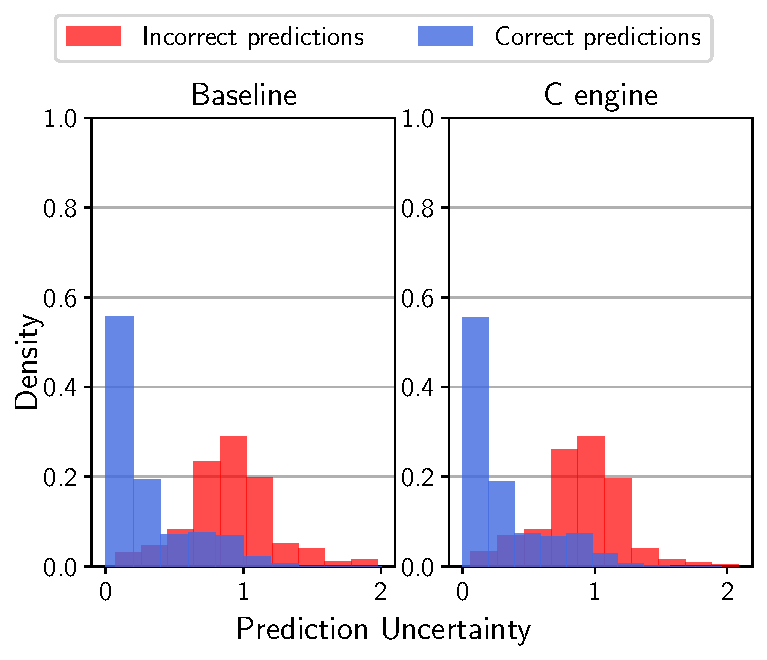
\includegraphics[width=\textwidth]{root/Imagenes/bnn_lib/hist_predictions.pdf}
     	\caption{Histogramas de incertidumbre divididos en predicciones correctas (azul) y predicciones incorrectas (rojo).}
     	\label{fig:example_hist}
 	\end{subfigure}
 	\hfill
 	\begin{subfigure}[b]{0.48\textwidth}
     	\centering
     	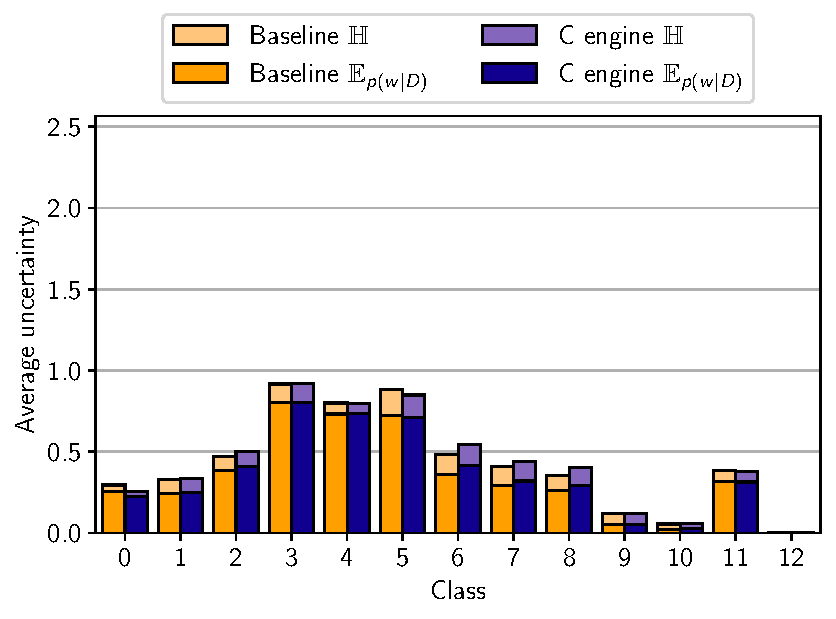
\includegraphics[width=\textwidth]{root/Imagenes/bnn_lib/class_uncertainty.pdf}
     	\caption{Incertidumbre predictiva ($\mathbb{H}$) y aleatoria ($\mathbb{E}p$) agrupada por clases.\\}
     	\label{fig:example_class}
 	\end{subfigure}
 	\hfill
 	\begin{subfigure}[b]{0.48\textwidth}
     	\centering
     	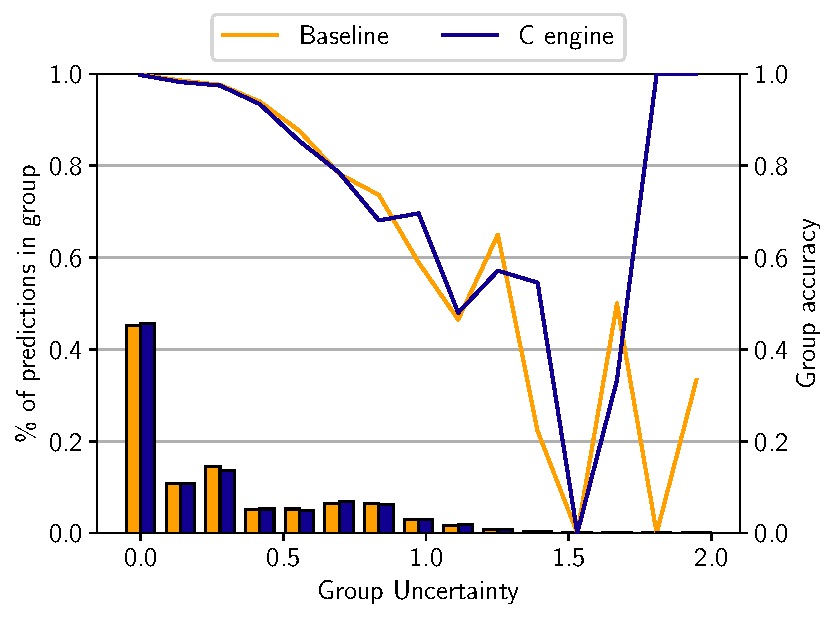
\includegraphics[width=\textwidth]{root/Imagenes/bnn_lib/acc_vs_unc.pdf}
     	\caption{Precisión y porcentaje de predicciones agrupadas por incertidumbre.\\}
     	\label{fig:example_acc_unc}
 	\end{subfigure}
 	\hfill
 	\begin{subfigure}[b]{0.48\textwidth}
     	\centering
     	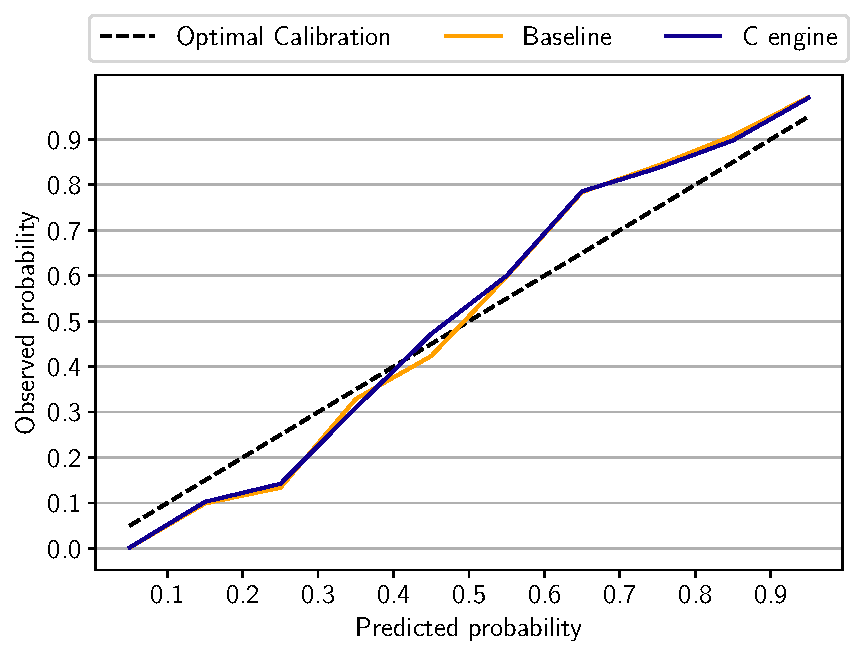
\includegraphics[width=\textwidth]{root/Imagenes/bnn_lib/calibration.pdf}
     	\caption{Recta de calibración del modelo, muestra probabilidades observadas con respecto a las probabilidades predichas por el modelo.}
     	\label{fig:example_calibration}
 	\end{subfigure}
    	\caption{Ejemplos de gráficas para analizar la incertidumbre y propiedades estadísticas de un modelo BNN. En \ref{fig:example_class}, \ref{fig:example_acc_unc} y \ref{fig:example_calibration} los colores amarillos representan los resultados obtenidos con TensorFlow y los colores azules los obtenidos con el motor de inferencia desarrollado. Predicciones del conjunto de prueba de píxeles hiperespectrales KSC.}
    	\label{fig:figure_example}
\end{figure}

Como se muestra en el ejemplo se obtienen resultados muy similares en todas las gráficas. Las únicas diferencias notables se aprecian en las rectas de precisión de la Figura \ref{fig:example_acc_unc}, pero estas diferencias ocurren en predicciones con incertidumbre alta de las que además hay muy pocas. El modelo al reportar una incertidumbre elevada ya está avisando de la baja fiabilidad de la predicción con lo que las diferencias en este tipo de predicciones son esperables y aceptables. Para el resto de modelos se obtienen resultados con las mismas similitudes entre motores de inferencia, se pueden consultar todos en el Anexo \ref{}. \todo

La Tabla \ref{tab:engine_acc} muestra la precisión obtenida con los diferentes modelos utilizando ambos motores de inferencia. Al tratarse de modelos probabilísticos pequeñas fluctuaciones son esperables, especialmente en las predicciones con mucha incertidumbre.

\begin{table}[ht]
\centering
\caption{Comparación de precisión obtenida con el motor de inferencia implementado con respecto a resultados obtenidos con TensorFlow}
\label{tab:engine_acc}
\begin{tabular}{lll}
\hline
 &  \multicolumn{2}{c}{\textbf{Motor de inferencia}}\\
 \textbf{Modelo} & \textit{TensorFlow} & \textit{C} \\ \hline
 Hiperespectral BO   & 0.9039 & 0.9101 \\
 Hiperespectral IP   & 0.8139 & 0.8148 \\
 Hiperespectral KSC  & 0.9256 & 0.9217 \\
 Hiperespectral PU   & 0.9017 & 0.9021 \\
 Hiperespectral SV   & 0.9257 & 0.9275 \\
 Lenet-5 MNIST  	& 0.9836 & 0.9830 \\
 Lenet-5 CIFAR10	& 0.6351 & 0.6229 \\
 B2N2 MNIST     	& 0.9872 & 0.9854 \\
 B2N2 CIFAR10   	& 0.7295 & 0.7134 \\\hline
\end{tabular}
\end{table}

Los resultados demuestran que el motor de inferencia desarrollado incluso tras transformar los datos a coma fija y perder precisión en la representación no perjudica a las métricas de incertidumbre ni a la precisión.

\section{Análisis de la carga de trabajo}

La principal operación en la inferencia de NN es \textit{\textbf{M}ultiply–\textbf{AC}cumulate} (MAC), mostrada en la Ecuación \ref{eq:mac}. Una capa es un conjunto de neuronas, las entradas a una neurona $x_i$ se multiplican por sus pesos $w_i$ y se acumulan junto a al \textit{bias} $b$. Una capa no convolucional se puede representar como una única multiplicación de matriz por vector.
\begin{equation} \label{eq:mac}
b + \sum_{i=0}^N w_i x_i
\end{equation}

En el caso de las BNN estas operaciones MAC además requieren muestrear una distribución gaussiana, como se muestra en la Ecuación \ref{eq:bnn_mac}.
\begin{equation} \label{eq:bnn_mac}
b + \sum_{i=0}^N Sample(\mu_i, \sigma_i)\ x_i
\end{equation}

El procesador RISC-V tiene un contador de ciclos disponible llamado \texttt{mcycle}, lo que permite medir prestaciones con precisión a nivel de ciclo. Se ha utilizado este contador para crear un perfil de la carga de trabajo del motor de inferencia, el cual se muestra en la Figura \ref{fig:cycle_profile}.

\begin{figure}[h]
	\centering
	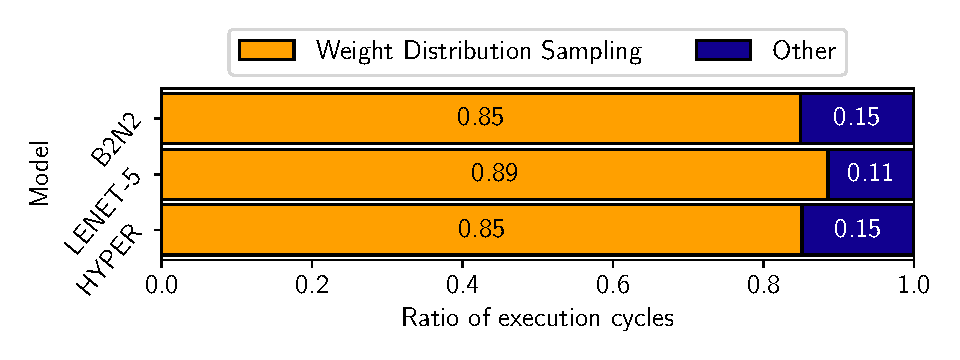
\includegraphics[width=0.9\textwidth]{root/Imagenes/bnn_lib/cycles.pdf}
	\caption{Ratio de ciclos de ejecución dedicados al muestreo de distribuciones gaussianas (amarillo) y al del resto de operaciones (azul) en las diferentes arquitecturas de modelos utilizadas.}
	\label{fig:cycle_profile}
\end{figure}

La operación de muestreo es la más costosa con diferencia, ocupando más del 80\% de los ciclos en los 3 modelos diferentes. Por ello, uno de los objetivos principales de este trabajo y de otros relacionados ha sido optimizar esta sección.

\chapter{Optimizaciones software}

\section{Optimización mediante distribuciones Bernoulli}

Awano \emph{et al.} \cite{bnn_clt_approx} propusieron muestrear distribuciones Bernoulli en vez de distribuciones gaussianas para aumentar la eficiencia del algoritmo en un acelerador para inferencia. Los parámetros de estas nuevas distribuciones se obtienen mediante una transformación de los parámetros de las distribuciones originales. A continuación se explican los fundamentos teóricos de esta optimización.

El TCL expone que en condiciones generales la distribución de una suma de variables aleatorias tiende a ser una distribución gaussiana. Las operaciones MAC son una suma de variables aleatorias por lo que según el TCL el resultado seguirá una distribución gaussiana. Una distribución gaussiana se define con 2 parámetros, la media y la desviación típica. Asumiendo que el tipo de distribución resultante es independiente del tipo de distribuciones de los sumandos, solamente se tiene que preservar la esperanza y la varianza de la operación MAC para no alterar los resultados de la BNN. Las Ecuaciones \ref{eq:neuron_expected}  y \ref{eq:neuron_variance} muestran la esperanza y la varianza de una operación MAC.
\begin{equation} \label{eq:neuron_expected}
E\left[ b + \sum_{i=0}^N w_i x_i \right]  = b + \sum_{i=0}^N ( E[w_i] E[x_i] )
\end{equation}
\begin{equation} \label{eq:neuron_variance}
V\left[ b + \sum_{i=0}^N w_i x_i \right] = \sum_{i=0}^N ( V[w_i]V[x_i] + V[w_i]E[x_i]^2 + V[x_i]E[w_i]^2 )
\end{equation}

La optimización consiste en utilizar un nuevo peso $w'$ que cumpla $E[w'] = E[w]$ y $V[w'] = V[w]$, de forma que no altere los resultados de la BNN. $w' = q \cdot b$, siendo $b$ una muestra de una distribución Bernoulli $\mathcal{B}(p)$, esta distribuciones toma el valor 1 con probabilidad $p$ y el valor 0 


y $a$ y $b$ siendo constantes que se pueden calcular a partir de la media $\mu$ y desviación típica $\sigma$ de los pesos originales utilizando el sistema de ecuaciones mostrado en la Ecuación \ref{eq:a_b_equation}.

En este trabajo se ha implementado esta optimización mediante software y se han analizado sus efectos sobre la precisión y métricas de incertidumbre.

\begin{figure}[h]
     \centering
     \begin{subfigure}[b]{0.46\textwidth}
         \centering
         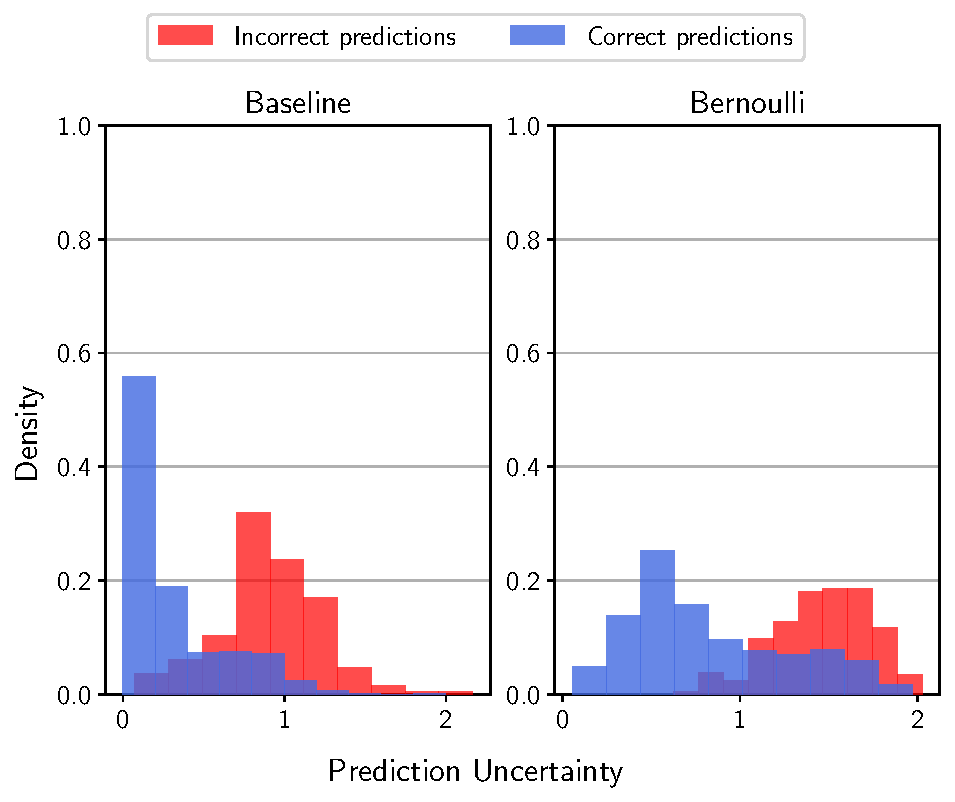
\includegraphics[width=\textwidth]{root/Imagenes/opt_software/bernoulli_hist.pdf}
         \caption{Histogramas de incertidumbre divididos en predicciones correctas (azul) y predicciones incorrectas (rojo).\\ \\}
         \label{fig:bernoulli_hist}
     \end{subfigure}
     \hfill
     \begin{subfigure}[b]{0.51\textwidth}
         \centering
         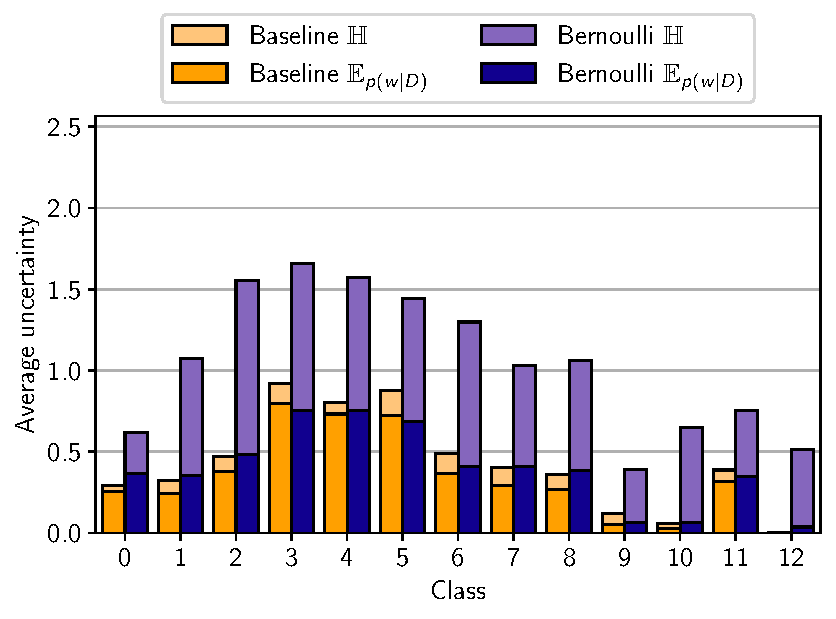
\includegraphics[width=\textwidth]{root/Imagenes/opt_software/bernoulli_class.pdf}
         \caption{Incertidumbre predictiva ($\mathbb{H}$) y aleatoria ($\mathbb{E}p$) agrupada por clases de los resultados obtenidos con TensorFlow (amarillo) y mediante la optimización basada en distribuciones de Bernoulli (azul).}
         \label{fig:bernoulli_class}
     \end{subfigure}
     \caption{Gráficas de análisis de incertidumbre de las predicciones del conjunto de prueba de píxeles hiperespectrales KSC, optimizados mediante distribuciones de Bernoulli y obtenidos mediante TensorFlow.}
     \label{fig:bernoulli}
\end{figure}

Esta degradación de las métricas hace que este modelo pierda una de las principales ventajas de utilizar una BNN por lo que no tiene sentido utilizarlo.

\section{Optimización mediante distribuciones Uniformes}

Este trabajo partiendo de Awano \emph{et al.} propone un nuevo método que utiliza distribuciones Uniformes en vez de distribuciones Bernoulli. Se propone utilizar un nuevo peso $w'$ que cumpla $E[w'] = E[w]$ y $V[w'] = V[w]$, de forma que no altere los resultados de la BNN. $w' = bu + a$, siendo $u$ una muestra de una distribución Uniforme $\mathcal{U}(0,1)$ y $a$ y $b$ siendo constantes que se pueden calcular a partir de la media $\mu$ y desviación típica $\sigma$ de los pesos originales utilizando el sistema de ecuaciones mostrado en la Ecuación \ref{eq:a_b_equation}.
\begin{equation}\label{eq:a_b_equation}
\begin{cases}
\mu = \dfrac{b}{2} + a\\ \\
\sigma^2 = \dfrac{b^2}{12}
\end{cases}
\rightarrow\ 
\begin{cases}
a = \mu - \dfrac{b}{2}\\ \\
b = \sigma \sqrt{12}
\end{cases}
\end{equation}

Esta optimización no aumenta el tamaño de los modelos y no necesita muestrear distribuciones gaussianas sino uniformes, cuyo algoritmo de muestreo es mucho mas sencillo. La Tabla \ref{tab:uniform_opt} muestra los resultados de precisión y aceleración (\textit{speedup}) obtenidos con esta optimización para todas las arquitecturas de modelos y conjuntos de datos.

\begin{table}[h]
    \centering
    \caption{Resultados de precisión y \textit{speedup} obtenidos con la optimización desarrollada para todas las arquitectruas de modelos y conjuntos de datos.}
    \label{tab:uniform_opt}
    \begin{tabular}{llrrr}
    \hline
     \multirow{2}{*}{\textbf{Modelo}} & \textbf{Conjunto} & \multicolumn{2}{c}{\textbf{Precisión}} & \multirow{2}{*}{\textbf{Speedup}} \\
     & \multicolumn{1}{c}{\textbf{de datos}} & \multicolumn{1}{l}{\textit{TensorFlow}} & \multicolumn{1}{l}{\textit{Optimizado}} & \\ \hline
    \multirow{5}{*}{HYPER} & BO & 0.9039 & 0.9083 & \multirow{5}{*}{4.95} \\
     & IP & 0.8139 & 0.8131 & \\
     & KSC & 0.9256 & 0.9217 & \\
     & PU & 0.9017 & 0.9017 & \\
     & SV & 0.9257 & 0.9280 & \\ \hline
    \multirow{2}{*}{LENET-5} & MNIST & 0.9836 & 0.8906 & \multirow{2}{*}{5.88} \\
     & CIFAR-10 & 0.6351 & 0.4436 & \\ \hline
    \multirow{2}{*}{B2N2} & MNIST & 0.9872 & 0.0964 & \multirow{2}{*}{4.88} \\
     & CIFAR-10 & 0.7295 & 0.2873 & \\ \hline                  
    \end{tabular}
\end{table}

Esta optimización ofrece muy buenos resultados en el caso de los modelos para clasificación de píxeles hiperespectrales, no afectando negativamente a la precisión de los modelos y obteniendo un \textit{speedup} de 4.95. Por contrario, en las arquitecturas de modelos mas le pérdida de precisión es mayor, en el caso del modelo B2N2 llega a ser completamente inaceptable. En el caso del modelo LENET-5 MNIST la precisión obtenida aun puede considerarse lo suficientemente buena la Figura \ref{fig:bad_uncert} muestra como se han degradado las métricas de incertidumbre del modelo. 

%Esta degradación de las métricas hace que este modelo pierda una de las principales ventajas de utilizar una BNN por lo que no tiene sentido utilizarlo.


\begin{figure}[h]
     \centering
     \begin{subfigure}[b]{0.46\textwidth}
         \centering
         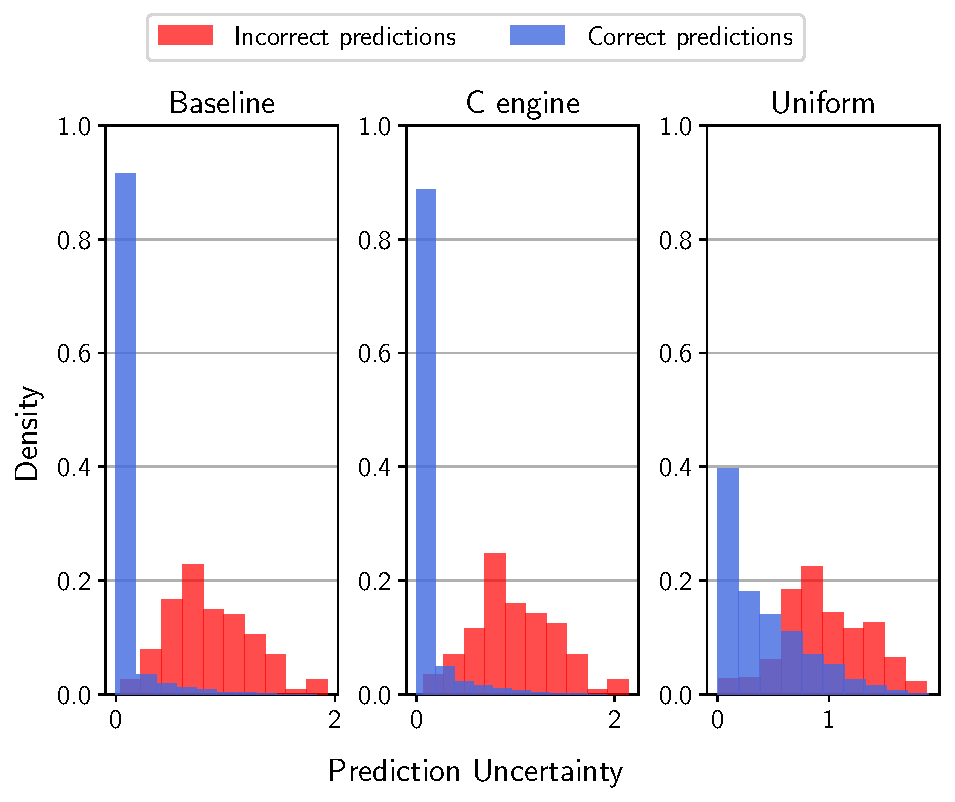
\includegraphics[width=\textwidth]{root/Imagenes/opt_software/hist_uncertainty.pdf}
         \caption{Histogramas de incertidumbre divididos en predicciones correctas (azul) y predicciones incorrectas (rojo).\\}
         \label{fig:bad_uncert_hist}
     \end{subfigure}
     \hfill
     \begin{subfigure}[b]{0.51\textwidth}
         \centering
         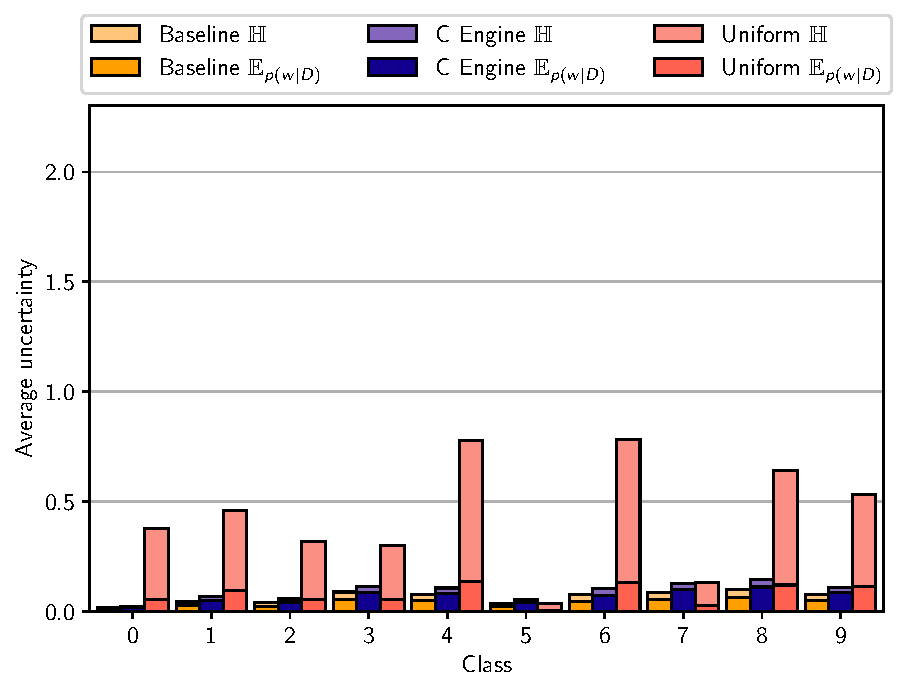
\includegraphics[width=\textwidth]{root/Imagenes/opt_software/class_uncertainty.pdf}
         \caption{Incertidumbre predictiva ($\mathbb{H}$) y aleatoria ($\mathbb{E}p$) agrupada por clases de los resultados obtenidos con TensorFlow (amarillo), el motor de inferencia sin optimización (azul) y con optimización (rojo).}
         \label{fig:bad_uncert_class}
     \end{subfigure}
     \caption{Gráficas de análisis de incertidumbre de los resultados del modelo LENET-5 MNIST optimizado, sin optimizar y obtenidos mediante TensorFlow.}
     \label{fig:bad_uncert}
\end{figure}

\chapter{Extensión RISC-V para inferencia de Redes Neuronales Bayesianas} \label{ch:extension}

\section{Diseño de una nueva unidad funcional}

Como se ha explicado en secciones previas, la sección del algoritmo mas importante a optimizar es el muestreo de distribuciones gaussianas. Para ello se va incluir un GRNG como una nueva unidad funcional (UF) en la CPU RISC-V base. Sarwar Malik \emph{et al.} propusieron un diseño basado en el TCL que añadía un componente corrector para reducir el error de muestreo de las colas de la distribución \cite{clt_grng} . Como también se ha mostrado previamente, no es necesaria una gran precisión a la hora de muestrear distribuciones, por lo que se va a diseñar un GNRG basado en la suma de 12 distribuciones uniformes sin bloque corrector. 

Se ha optado por utilizar un GRNG y no un generador de otro tipo como el que requieren alguna de las optimizaciones software para desviarse lo menos posible del algoritmo original y crear una UF que pueda ser útil para otro tipo de aplicaciones que requieran muestrear distribuciones Gaussianas.

\subsection{Generador de números pseudoaleatorios uniformes}

Para generar números pseudoaletorios uniformes se ha utilizado un componente hardware llamado \textit{\textbf{L}inear \textbf{F}eedback \textbf{S}hift \textbf{R}egister} (LFSR). Se basan en un circuito de retroalimentación y un registro de estado. El circuito de retroalimentación es un conjunto de puertas XOR que implementan un polinomio generador. Dado un registro de estado de $n$ bits, si el polinomio puede producir $2^n-1$ valores a
ntes de empezar a repetir la secuencia entonces la secuencia es máxima. Alfke recopiló una lista de polinomios generadores para secuencias máximas para varios tamaños de registros de estado \cite{lfsr_poly}. La desventaja de este tipo de LFSR es que no pueden generar más de un bit con baja correlación entre muestras. La Figura \ref{fig:lfsr_bar_corr} muestra diagramas de muestras con alta correlación, el diagrama de autocovarianza debería mostrar un único pico en el 0 y el gráfico de dispersión un patrón de ruido blanco.

\begin{figure}[h]
    \centering
    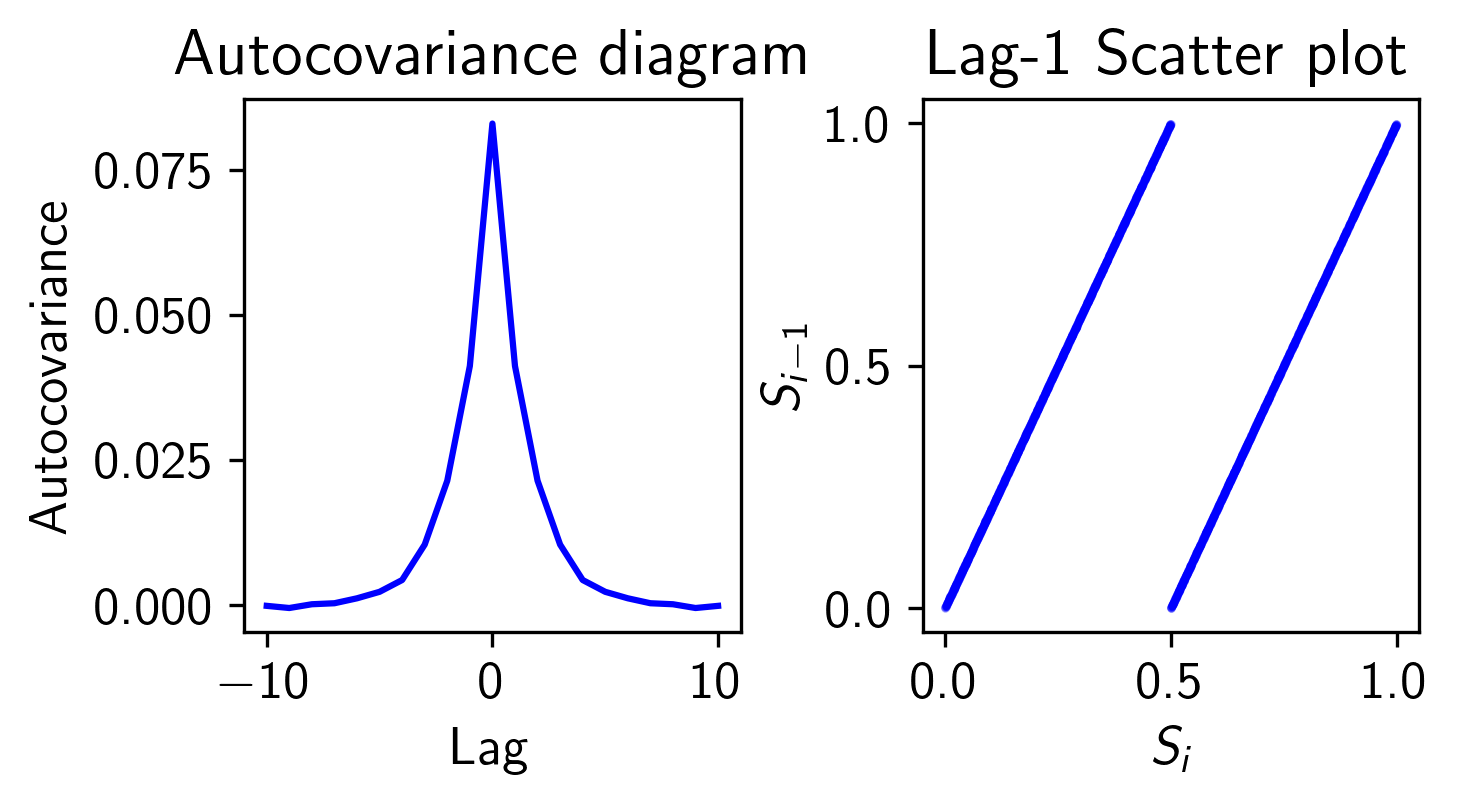
\includegraphics[width=0.7\textwidth]{root/Imagenes/riscv_ext/lfsr_bar_corr.png}
    \caption{Diagramas de correlación de $10^4$ muestras de 12 bits de un LFSR. A la izquierda un diagrama de autocovarianza para diferentes distancias entre muestras. A la derecha un diagrama de dispersión de una muestra $i$ con respecto a la $i-1$.}
    \label{fig:lfsr_bar_corr}
\end{figure}

Para paliar este problema se ha utilizado un \textit{Lookahead} LFSR \cite{look_ahead_lfsr_base}. Estos LFSR tienen un circuito de retroalimentación más complejo que generan $n$ bits con baja correlación. Este circuito aplica el polinomio generador base $n$ veces, Colavito \emph{et al.} detallaron como obtener estos circuitos mediante exponenciación de matrices y que restricciones deben seguir \cite{look_ahead_lfsr_design}. En este trabajo se ha desarrollado un \textit{script} en Python que genera código VHDL para implementar \textit{Lookahead} LFSR utilizando su método. La Figura \ref{fig:lfsr_good_corr} muestra los diagramas de correlación que se obtienen utilizando este tipo de LFSR.

\begin{figure}[h]
    \centering
    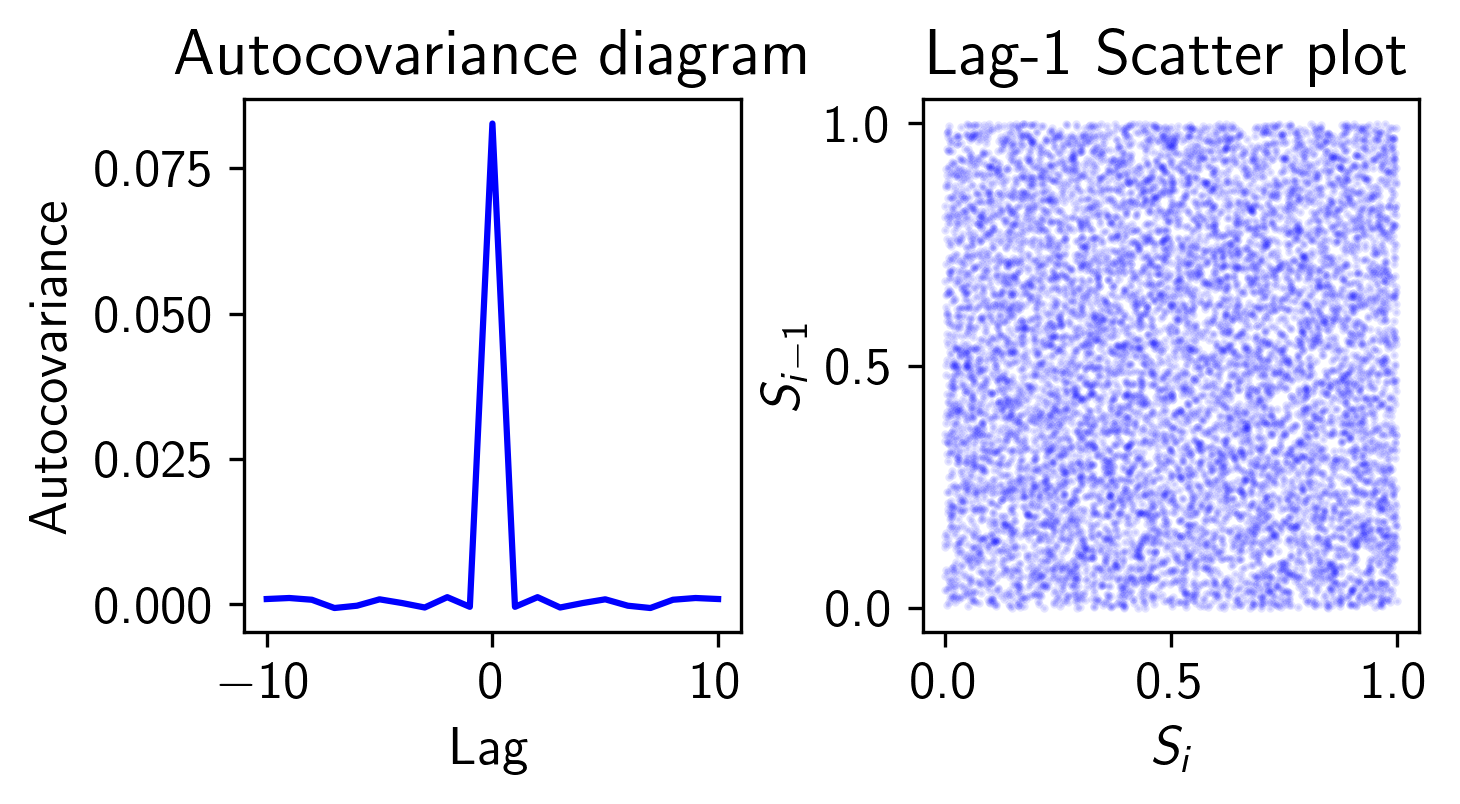
\includegraphics[width=0.7\textwidth]{root/Imagenes/riscv_ext/lfsr_good_corr.png}
    \caption{Diagramas de correlación de $10^4$ muestras de 12 bits de un 12-\textit{Lookahead} LFSR. A la izquierda un diagrama de autocovarianza para diferentes distancias entre muestras. A la derecha un diagrama de dispersión de una muestra $i$ con respecto a la $i-1$.}
    \label{fig:lfsr_good_corr}
\end{figure}

\subsection{Generador de números pseudoaleatorios gaussianos}

Un GRNG basado en el TCL tiene 2 componentes principales, un generador de muestras de distribuciones uniformes y un árbol de sumadores que las acumula. Para sumar 12 muestras se necesita un árbol de 4 niveles. Como se busca obtener una muestra final de 16 bits las muestras iniciales deben ser de 12 bits, ya que por cada nivel del árbol las muestras aumentan su tamaño en 1 bit para evitar problemas de desbordamiento. Para evitar afectar negativamente a la frecuencia del reloj de la CPU original el árbol se ha segmentado por niveles, lo que permite obtener una muestra por ciclo. Solamente penalizando en el cambio de semilla, que hay que esperar 4 ciclos para obtener muestras con la semilla actualizada.

Para generar 12 muestras de 12 bits se utiliza un 144-\textit{Lookahead} LFSR con un registro de estado de 151 bits. Las muestras representan valores entre 0 y 1, codificados en coma fija con una escala $2^{12}$. Para centrar la muestra final se utiliza un restador de 16 bits con un valor constante $6 \cdot 2^{12}$. La Figura \ref{fig:grng} muestra un diagrama del diseño y la Figura \ref{fig:grng_state} la máquina de estados de su unidad de control.

\begin{figure}[h]
    \centering
    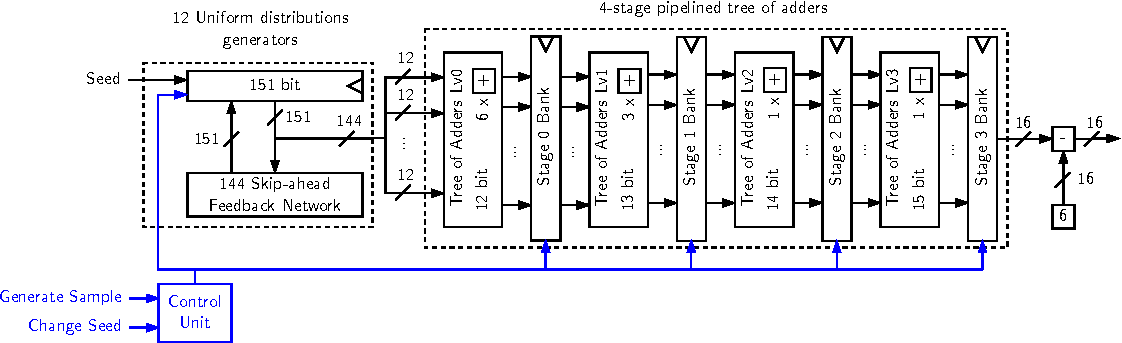
\includegraphics[width=\textwidth]{root/Imagenes/riscv_ext/grng.pdf}
    \caption{Diagrama del GRNG implementado. Las señales de control se muestran en azul, las de datos en negro.}
    \label{fig:grng}
\end{figure}

\begin{figure}[h]
    \centering
    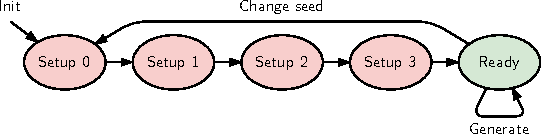
\includegraphics[width=0.8\textwidth]{root/Imagenes/riscv_ext/grng_states.pdf}
    \caption{Diagrama de estados de la unidad de control del GRNG. El estado en el que se pueden generar muestras válidas esta marcado en verde, el resto en rojo.}
    \label{fig:grng_state}
\end{figure}

\section{Modificaciones del procesador RISC-V base}

El GRNG diseñado se ha integrado en la CPU original como una nueva UF en la etapa \textit{Execute}. Para ello se ha modificado la etapa de \textit{Decode} para añadir 2 nuevas instrucciones y el selector de resultado de la etapa \textit{Execute}. La Figura \ref{fig:extended_riscv_core} muestra un diagrama de la ruta de datos 

\begin{figure}[h]
    \centering
    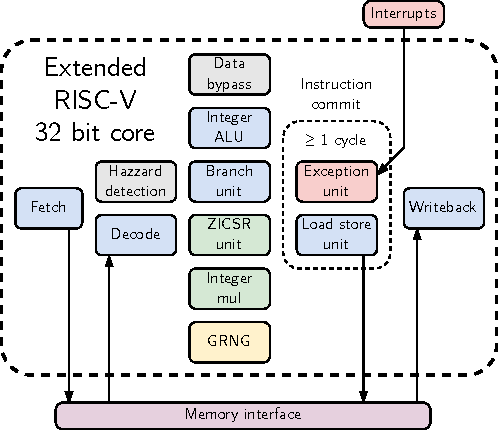
\includegraphics[width=0.75\textwidth]{root/Imagenes/riscv_ext/extended_core.pdf}
    \caption{Ruta de datos del procesador RISC-V extendido con el GRNG, mostrado en amarillo. Los bloques relacionados con la arquitectura base RV32I se muestran en azul, los bloques para detectar riesgos de datos en gris, los bloques relacionados con el modo M en rojo, los bloques de extensiones estándar extra en verde y en morado el interfaz con el bus de memoria.}
    \label{fig:extended_riscv_core}
\end{figure}



Otra opción posible habría sido añadirlo como un periférico que se accediera mediante entrada y salida mapeada en memoria (\textit{\textbf{M}emory \textbf{M}apped \textbf{I}nput \textbf{O}utput}), pero esta fue descartada por los siguientes motivos. Implicaría que se accedería mediante instrucciones \texttt{load} y \texttt{store}, lo que reduciría el rendimiento ya que estas instrucciones no permiten consumidores a distancia 1. Además el acceso a memoria generalmente requiere circuitos mas complejos por lo que estas instrucciones pueden tener un coste mas elevado, esto no ocurre en la CPU base, cuyo acceso a memoria es lo más simple posible, pero esto si que podría ocurrir en otras CPU y afectar negativamente al rendimiento. Otro factor en contra de esta aproximación es que en el futuro se quiere crear una UF mas compleja que utilice el GRNG.

\section{Actualización del compilador gcc con nuevas instrucciones}

Para poder utilizar el GRNG se han añadido 2 instrucciones nuevas al repertorio RISC-V. El objetivo de estas nuevas instrucciones es acelerar el motor de inferencia que se ha desarrollado, por lo que se han de poder utilizar desde código de alto nivel en C. Por lo que se ha actualizado el compilador \texttt{gcc} para RISC-V, lo que se ha podido hacer gracias a que es de código abierto. A continuación se describen las instrucciones añadidas:
\begin{itemize}
    \item \texttt{setseed rs1}. Cambia la semilla por el valor del registro \texttt{rs1}.
    \item \texttt{genum rd}. Genera una muestra de $\mathcal{N}(0,1)$ y la guarda en los 16 bits mas altos del registro \texttt{rd}. Eso implica que la muestra está codificada en coma fija en escala $2^{12 + 16}$.
\end{itemize}

Para poder actualizar el compilador hay que definir la codificación de las instrucciones siguiendo las directrices de RISC-V. Además hay que definir una máscara junto con un valor para que \texttt{gcc} pueda comprobar la codificación mediante una operación \texttt{and}. Para ambas instrucciones se ha utilizado la codificación de instrucciones tipo R de RISC-V y se muestran en las Tablas \ref{tab:code_setseed} y \ref{tab:code_genum}.

\begin{table}[h]
    \centering
    \caption{Codificación, máscara y validación de la instrucción \texttt{setseed} separada en los campos de instrucción RISC-V tipo R.}
    \label{tab:code_setseed}
    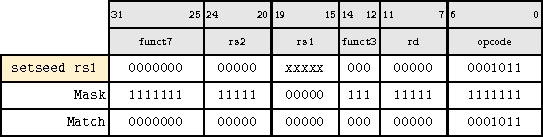
\includegraphics[width=0.85\textwidth]{root/Imagenes/riscv_ext/code_setseed.pdf}
\end{table}

\begin{table}[h]
    \centering
    \caption{Codificación, máscara y validación de la instrucción \texttt{genum} separada en los campos de instrucción RISC-V tipo R.}
    \label{tab:code_genum}
    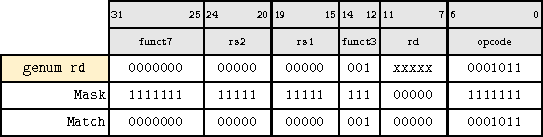
\includegraphics[width=0.85\textwidth]{root/Imagenes/riscv_ext/code_genum.pdf}
\end{table}

%%%%%

\section{Análisis de resultados}

Utilizando la extensión desarrollada no degrada la precisión ni las métricas de incertidumbre con respecto a los resultados obtenidos con el motor de inferencia en C, ya que el algoritmo de muestreo es el mismo. La Tabla \ref{tab:riscv_speedup} muestra el \textit{speedup} obtenido con todas las optimizaciones desarrolladas en este trabajo para todas las arquitecturas de modelos. Utilizando la nueva UF se obtiene el mejor rendimiento.

\begin{table}[h]
    \centering
    \caption{\textit{Speedups} obtenidos con todas las optmizaciones desarrolladas en este trabajo para todas las arquitecturas de modelos.}
    \label{tab:riscv_speedup}
    \begin{tabular}{llll}
    \hline
    \multirow{2}{*}{\textbf{Modelo}} & \multicolumn{3}{c}{\textbf{Speedup}}\\
    & \textit{Bernoulli} & \textit{Uniforme} & \textit{Extensión}\\ \hline
    HYPER& 5.18 & 4.95 & 6.37 \\
    LENET-5& \todo & 5.88 & 8.10 \\
    B2N2& \todo & 4.88 & 6.24 \\ \hline
    \end{tabular}
\end{table}

\section{Análisis de coste}

Para analizar el coste de añadir la extensión a la CPU base se ha utilizado una FPGA. Una FPGA es un componente que permite implementar en hardware real circuitos lógicos definidos en un lenguaje de alto nivel como VHDL. Las FPGA estan compuestas por distintos tipos de bloques, las herramientas de síntesis transforman el diseño a estos bloques y configuran la red de interconexión de los mismos. Algunos tipos de bloques son LUT, registros (\textit{\textbf{F}lip-\textbf{F}lops}), memorias RAM (BRAM) o bloques para procesado de señal (\textit{\textbf{D}igital \textbf{S}ignal \textbf{P}rocessor}), que se pueden utilizar para realizar operaciones matemáticas complejas como la multiplicación. Utilizando una herramienta de síntesis se han obtenido los costes descritos en la Tabla \ref{tab:riscv_fpga_utilization}.

\begin{table}[h]
\centering
\caption{Utilización de recursos de la FPGA de la CPU base y la extensión.}
\label{tab:riscv_fpga_utilization}
\begin{tabular}{lrrr}
\hline
\multirow{2}{*}{\textbf{Tipo}} & \multicolumn{2}{c}{\textbf{Recursos Utilizados}} & \multirow{2}{*}{\textbf{Utilización FPGA \%}}\\
 & \textit{CPU Base} & \textit{Extensión GRNG} & \\ \hline
LUT	        & 2435 & 240 & 1.16 \\
FF	        & 1922 & 320 & 0.49 \\
BRAM	    & 16   & 0 & 5.13 \\
DSP	        & 12   & 0 & 0.69 \\ \hline
\end{tabular}
\end{table}

Añadir la extensión a la CPU base implica un incremento del 9.86 y del 16.65\% en LUTs y FFs. Hay que tener en cuenta que este coste además del GRNG incluye las modificaciones a la ruta de datos del procesador. Aun así el coste total de la CPU es muy bajo, no llegando a utilizar ni un 10\% de los bloques de la FPGA. Además al haber segmentado el GRNG este no tiene ningun efecto negativo en la frecuencia del reloj del diseño original, 100 MHz.

La herramienta de síntesis también calcula estimaciones del consumo energético del diseño implementado, dividiéndolo en estático y dinámico. La Tabla \ref{tab:riscv_fpga_power} muestra esta estimación. El consumo energético aumenta solamente en un 0.65\%. Por lo tanto, la extensión consigue una reducción en del consumo casi idéntica a la ganancia en rendimiento.

\begin{table}[h]
\centering
\caption{Estimación del consumo energético de la CPU base y extendida.}
\label{tab:riscv_fpga_power}
\begin{tabular}{lccc}
\hline
\multirow{2}{*}{\textbf{Tipo}} & \multicolumn{3}{c}{\textbf{Consumo Energético (W)}} \\
 & \textit{CPU Base} & \textit{Extensión GRNG} & Total \\ \hline
Dinámico & 0.023 & 0.004 & 0.027\\
Estático & 0.593 & 0.000 & 0.593\\ \hline
\end{tabular}
\end{table}

\chapter{Conclusiones} \label{ch:conclusion}

Este trabajo estudia la inferencia de BNN en dispositivos IoT de bajo consumo, utilizando como ejemplo un procesador RISC-V. Se han desarrollado herramientas de código abierto para transformar modelos BNN en punto flotante de TensorFlow a código C para inferencia utilizando solo precisión entera. Además, analiza diferentes métodos de optimización para el algoritmo de muestreo de pesos del algoritmo de inferencia, ya que consume la mayor parte del tiempo de ejecución.

Para acelerar la inferencia, este trabajo estudia el impacto en las métricas de incertidumbre y el coste de su implementación en software de una optimización propuesta en otro trabajo. Además este trabajo propone una nueva versión de dicha optimización que consiste en muestrear una distribución Uniforme. Esta optimización logra, en promedio, un \textit{speedup} de 5 en varios modelos representativos de BNN, conservando las métricas de incertidumbre en todos ellos.

Para mejorar estos resultados, se ha desarrollado una extensión para RISC-V que permite muestrear una distribución gaussiana usando solo una instrucción, implementada en un procesador de 32 bits. Las muestras se generan utilizando un GRNG basado en el TCL de bajo coste. La extensión acelera la inferencia hasta 7.65 veces, con reducciones similares en el consumo de energía y sin degradación significativa en la precisión o las métricas de incertidumbre. Se ha implementado el diseño en una FPGA Xilinx ZCU104. Su coste es solo de 240 LUTs y 320 Flip-Flops, generando un aumento del 0.65\% en el consumo de energía, sin afectar la frecuencia del reloj del sistema.

Como trabajo futuro se podría seguir iterando sobre la UF desarrollada permitiendo no solo generar muestras sino realizar toda la operación MAC requerida en la inferencia, lo que aumentaría aun mas el rendimiento. También se podría estudiar la portabilidad de la extensión desarrollada incluyéndola en otras CPU RISC-V abiertas. Por el lado del software, se podría añadir al motor desarrollado un marco de cuantización mas complejo, permitiendo reducir aun mas el tamaño de los modelos.


%%%%%%%%%%%%%%%%%%%%%%%%%%%%%%%%%%%%%%%%%%%%%%%%%%%%%%%%%%%%%%%%%%%%%%%%%%%%%%%%%%%
%		BIBLIOGRAFÍA Y REFERENCIAS
%%%%%%%%%%%%%%%%%%%%%%%%%%%%%%%%%%%%%%%%%%%%%%%%%%%%%%%%%%%%%%%%%%%%%%%%%%%%%%%%%%%

\bibliographystyle{unsrt} %plaindin
\bibliography{Bibliografia_TFM}
\nocite{*} 

\newpage
\renewcommand\listfigurename{Lista de Figuras}
\listoffigures

\newpage
\renewcommand\listtablename{Lista de Tablas}
\listoftables

%%%%%%%%%%%%%%%%%%%%%%%%%%%%%%%%%%%%%%%%%%%%%%%%%%%%%%%%%%%%%%%%%%%%%%%%%%%%%%%%%%%
%		ANEXOS
%%%%%%%%%%%%%%%%%%%%%%%%%%%%%%%%%%%%%%%%%%%%%%%%%%%%%%%%%%%%%%%%%%%%%%%%%%%%%%%%%%%

\newpage
\appendix
\clearpage
\addappheadtotoc
\appendixpage
\chapter{Resultados de incertidumbre del motor de inferencia} \label{anx:motor}

\begin{figure}[ht]
    \centering
    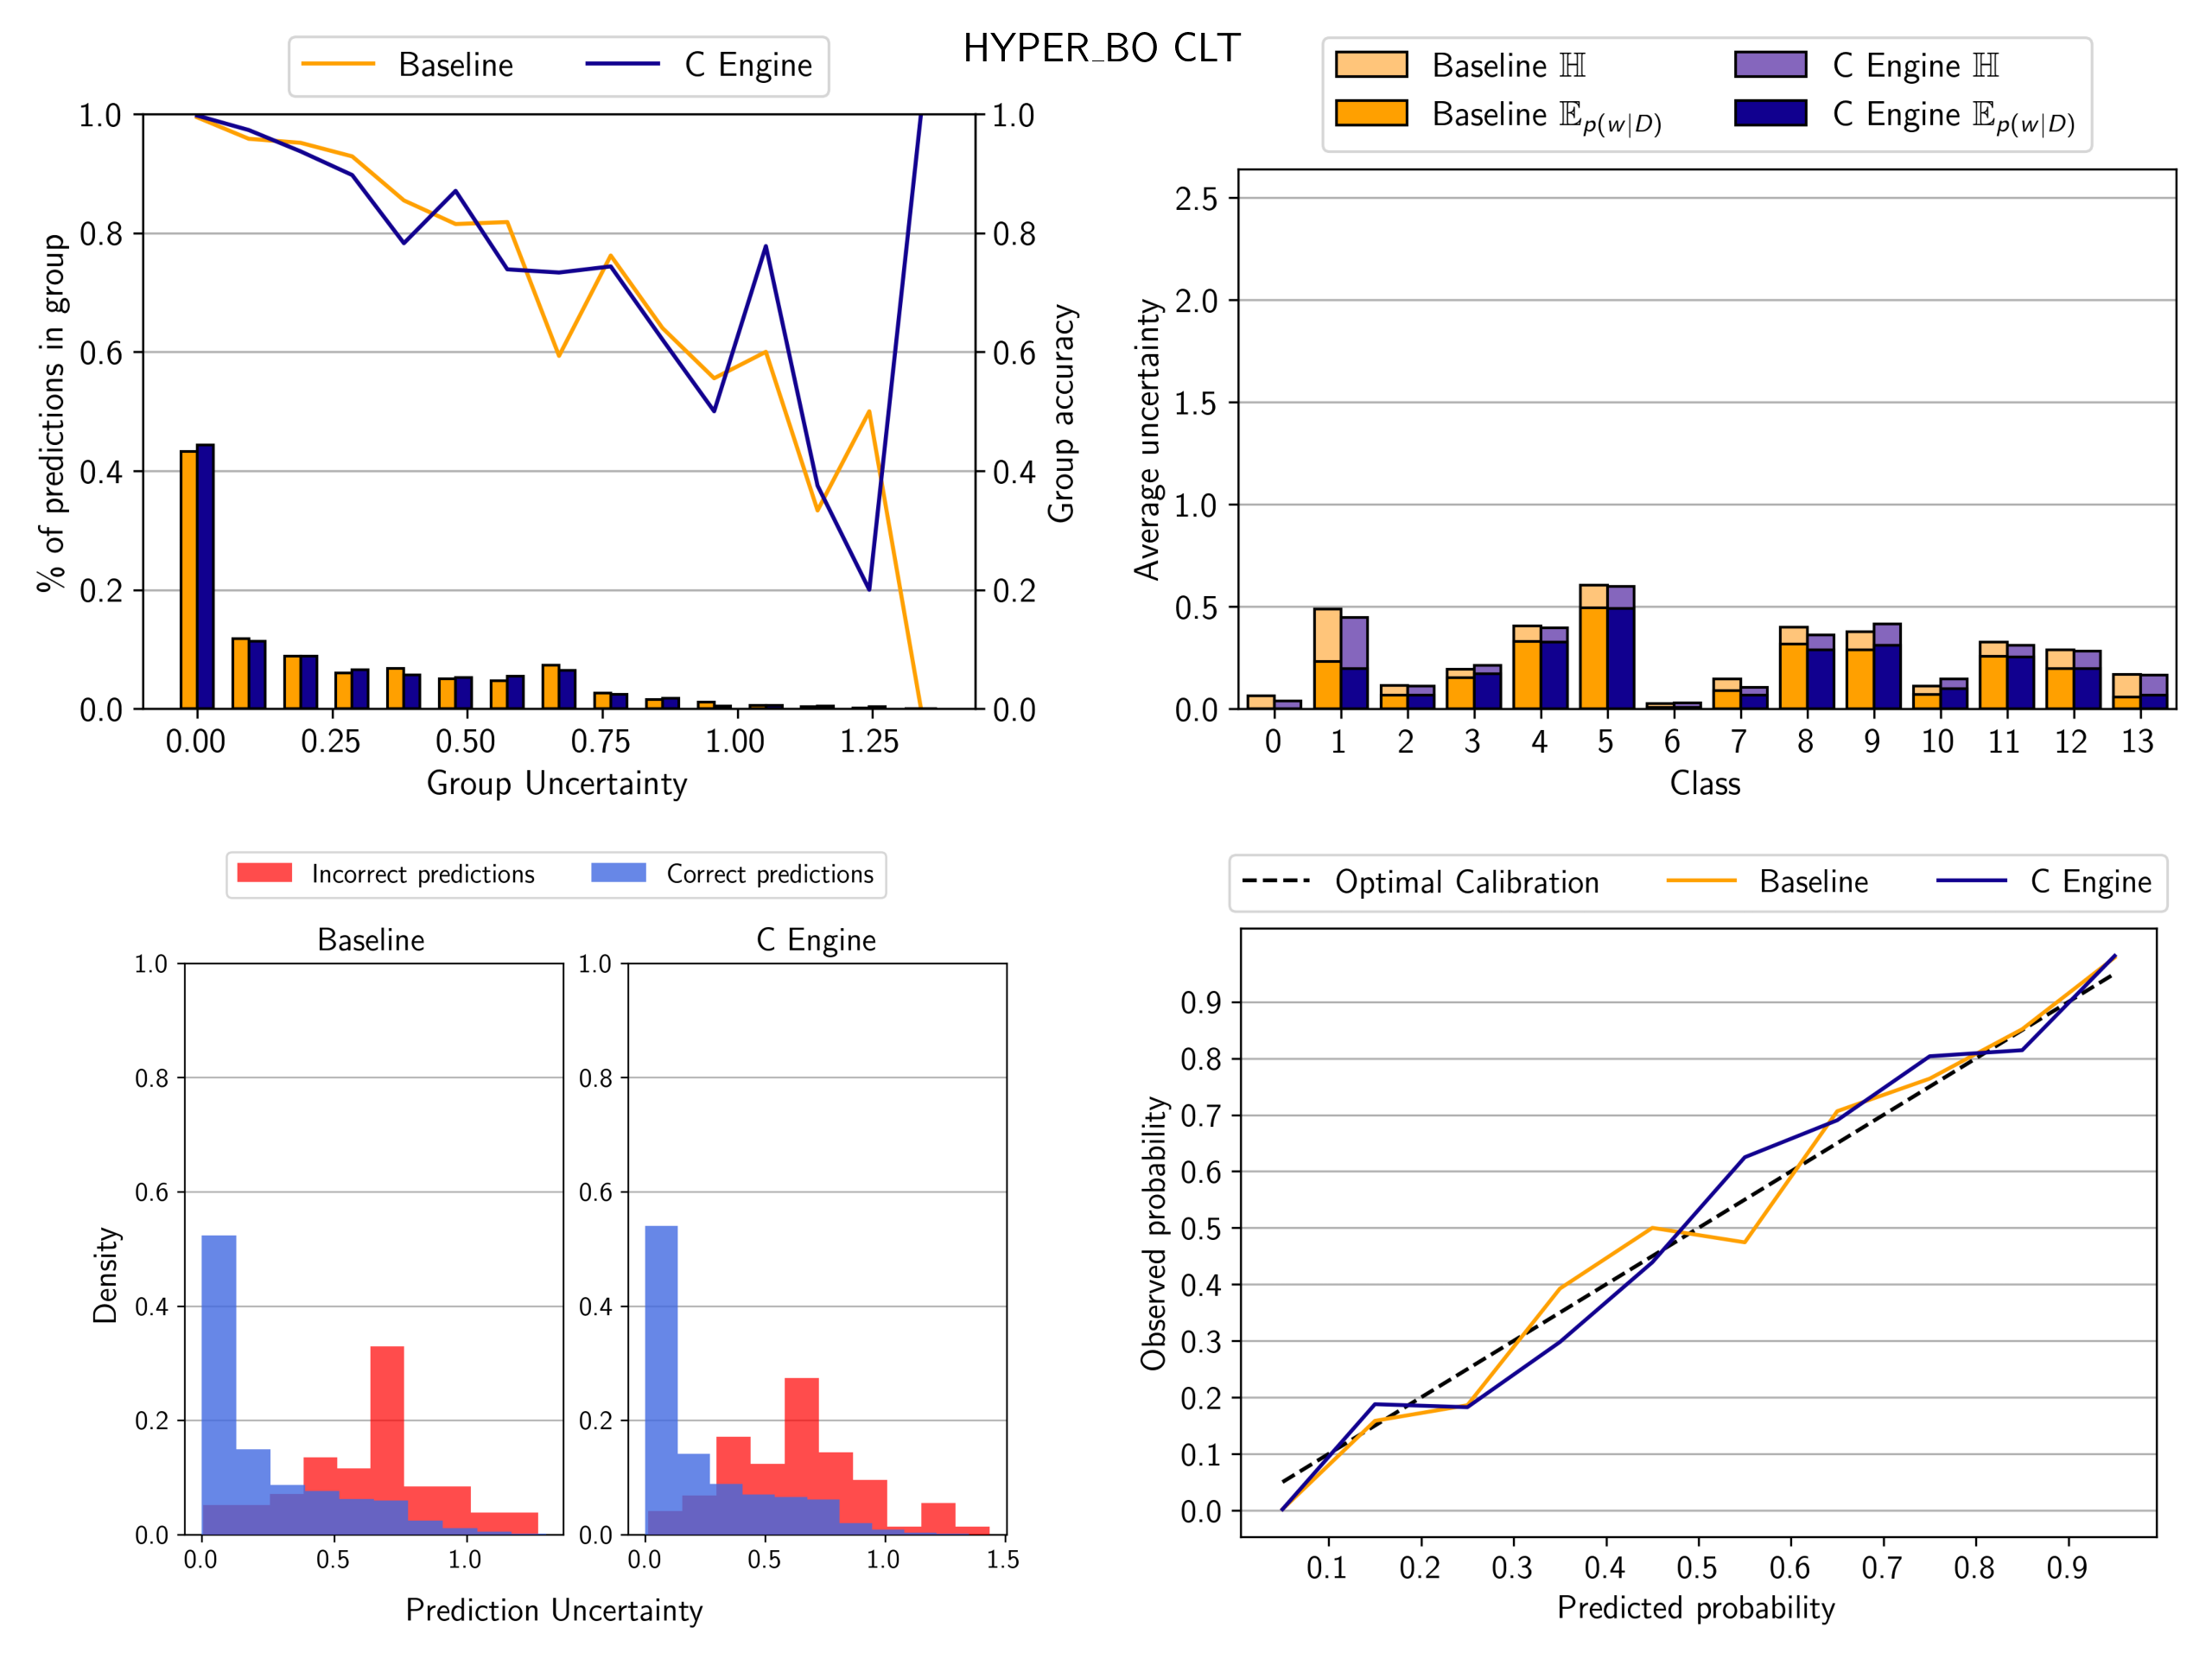
\includegraphics[width=0.9\textwidth]{root/Imagenes/anexo/CLT-HYPER_BO-mosaic.png}
    \caption{Predicciones del conjunto de prueba de píxeles hiperespectrales BO.}
    \label{fig:anx-CLT-HYPER_BO}
\end{figure}


\begin{figure}[ht]
    \centering
    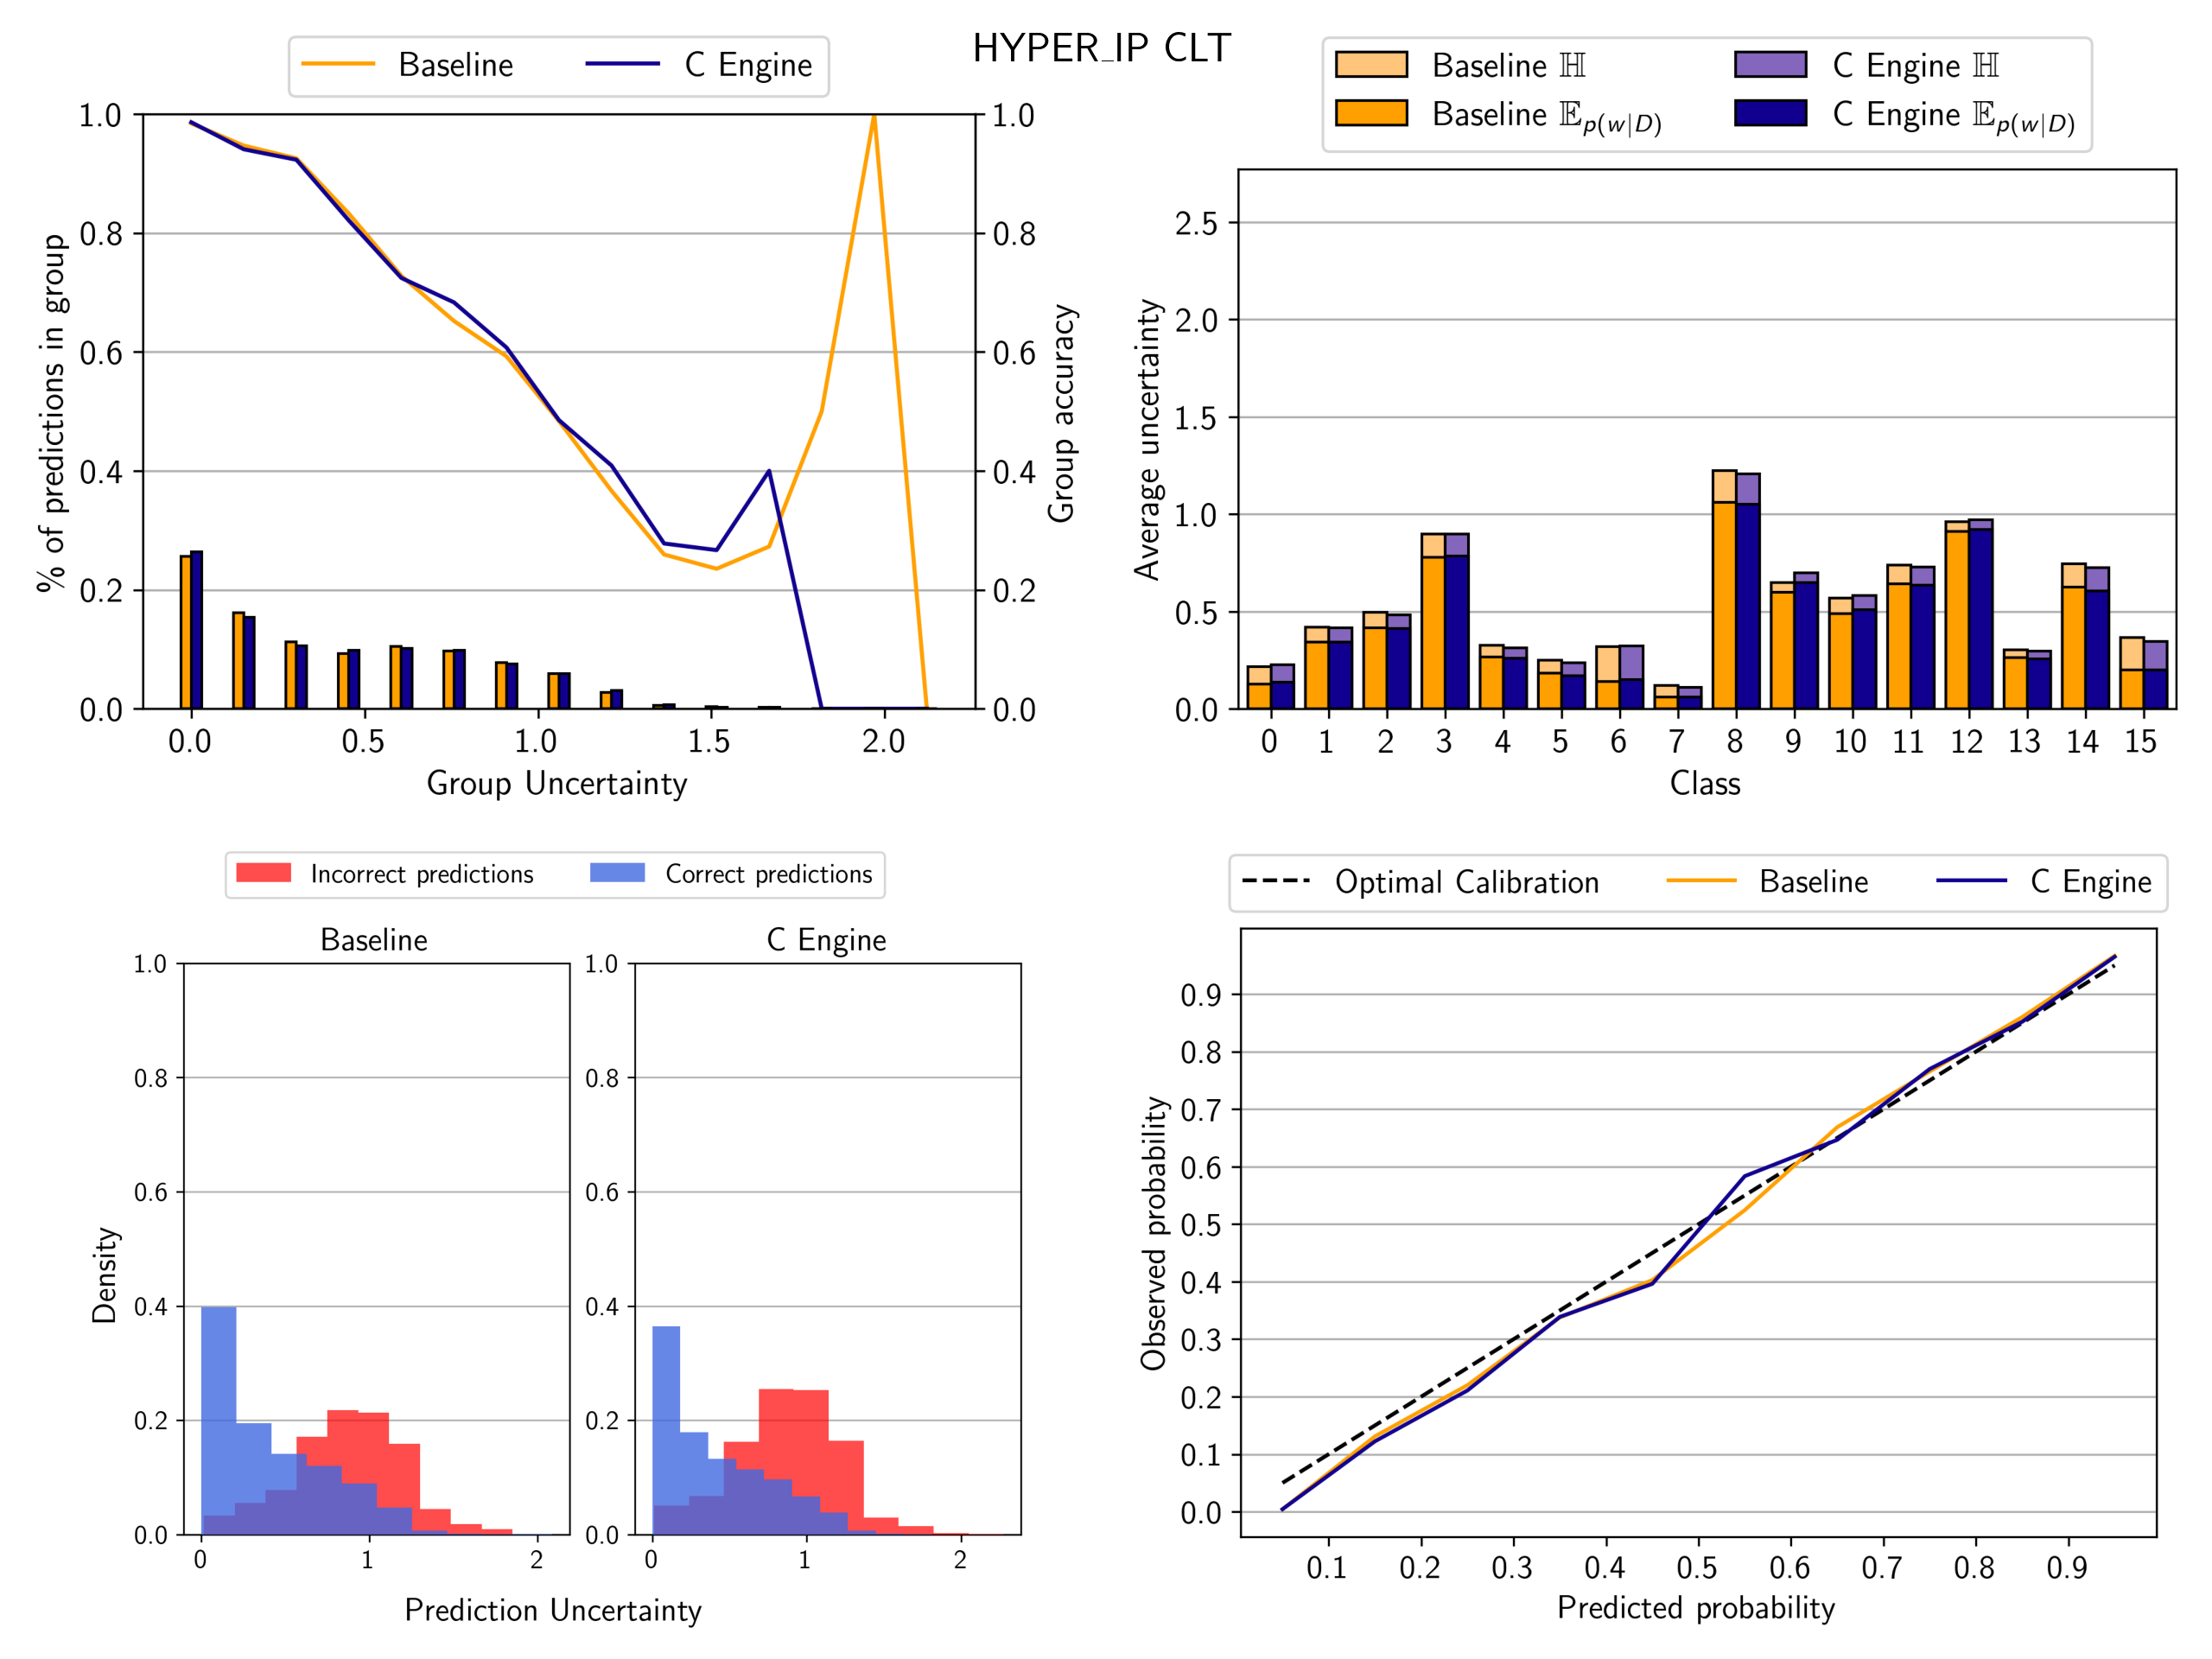
\includegraphics[width=0.9\textwidth]{root/Imagenes/anexo/CLT-HYPER_IP-mosaic.png}
    \caption{Predicciones del conjunto de prueba de píxeles hiperespectrales IP.}
    \label{fig:anx-CLT-HYPER_IP}
\end{figure}


\begin{figure}[ht]
    \centering
    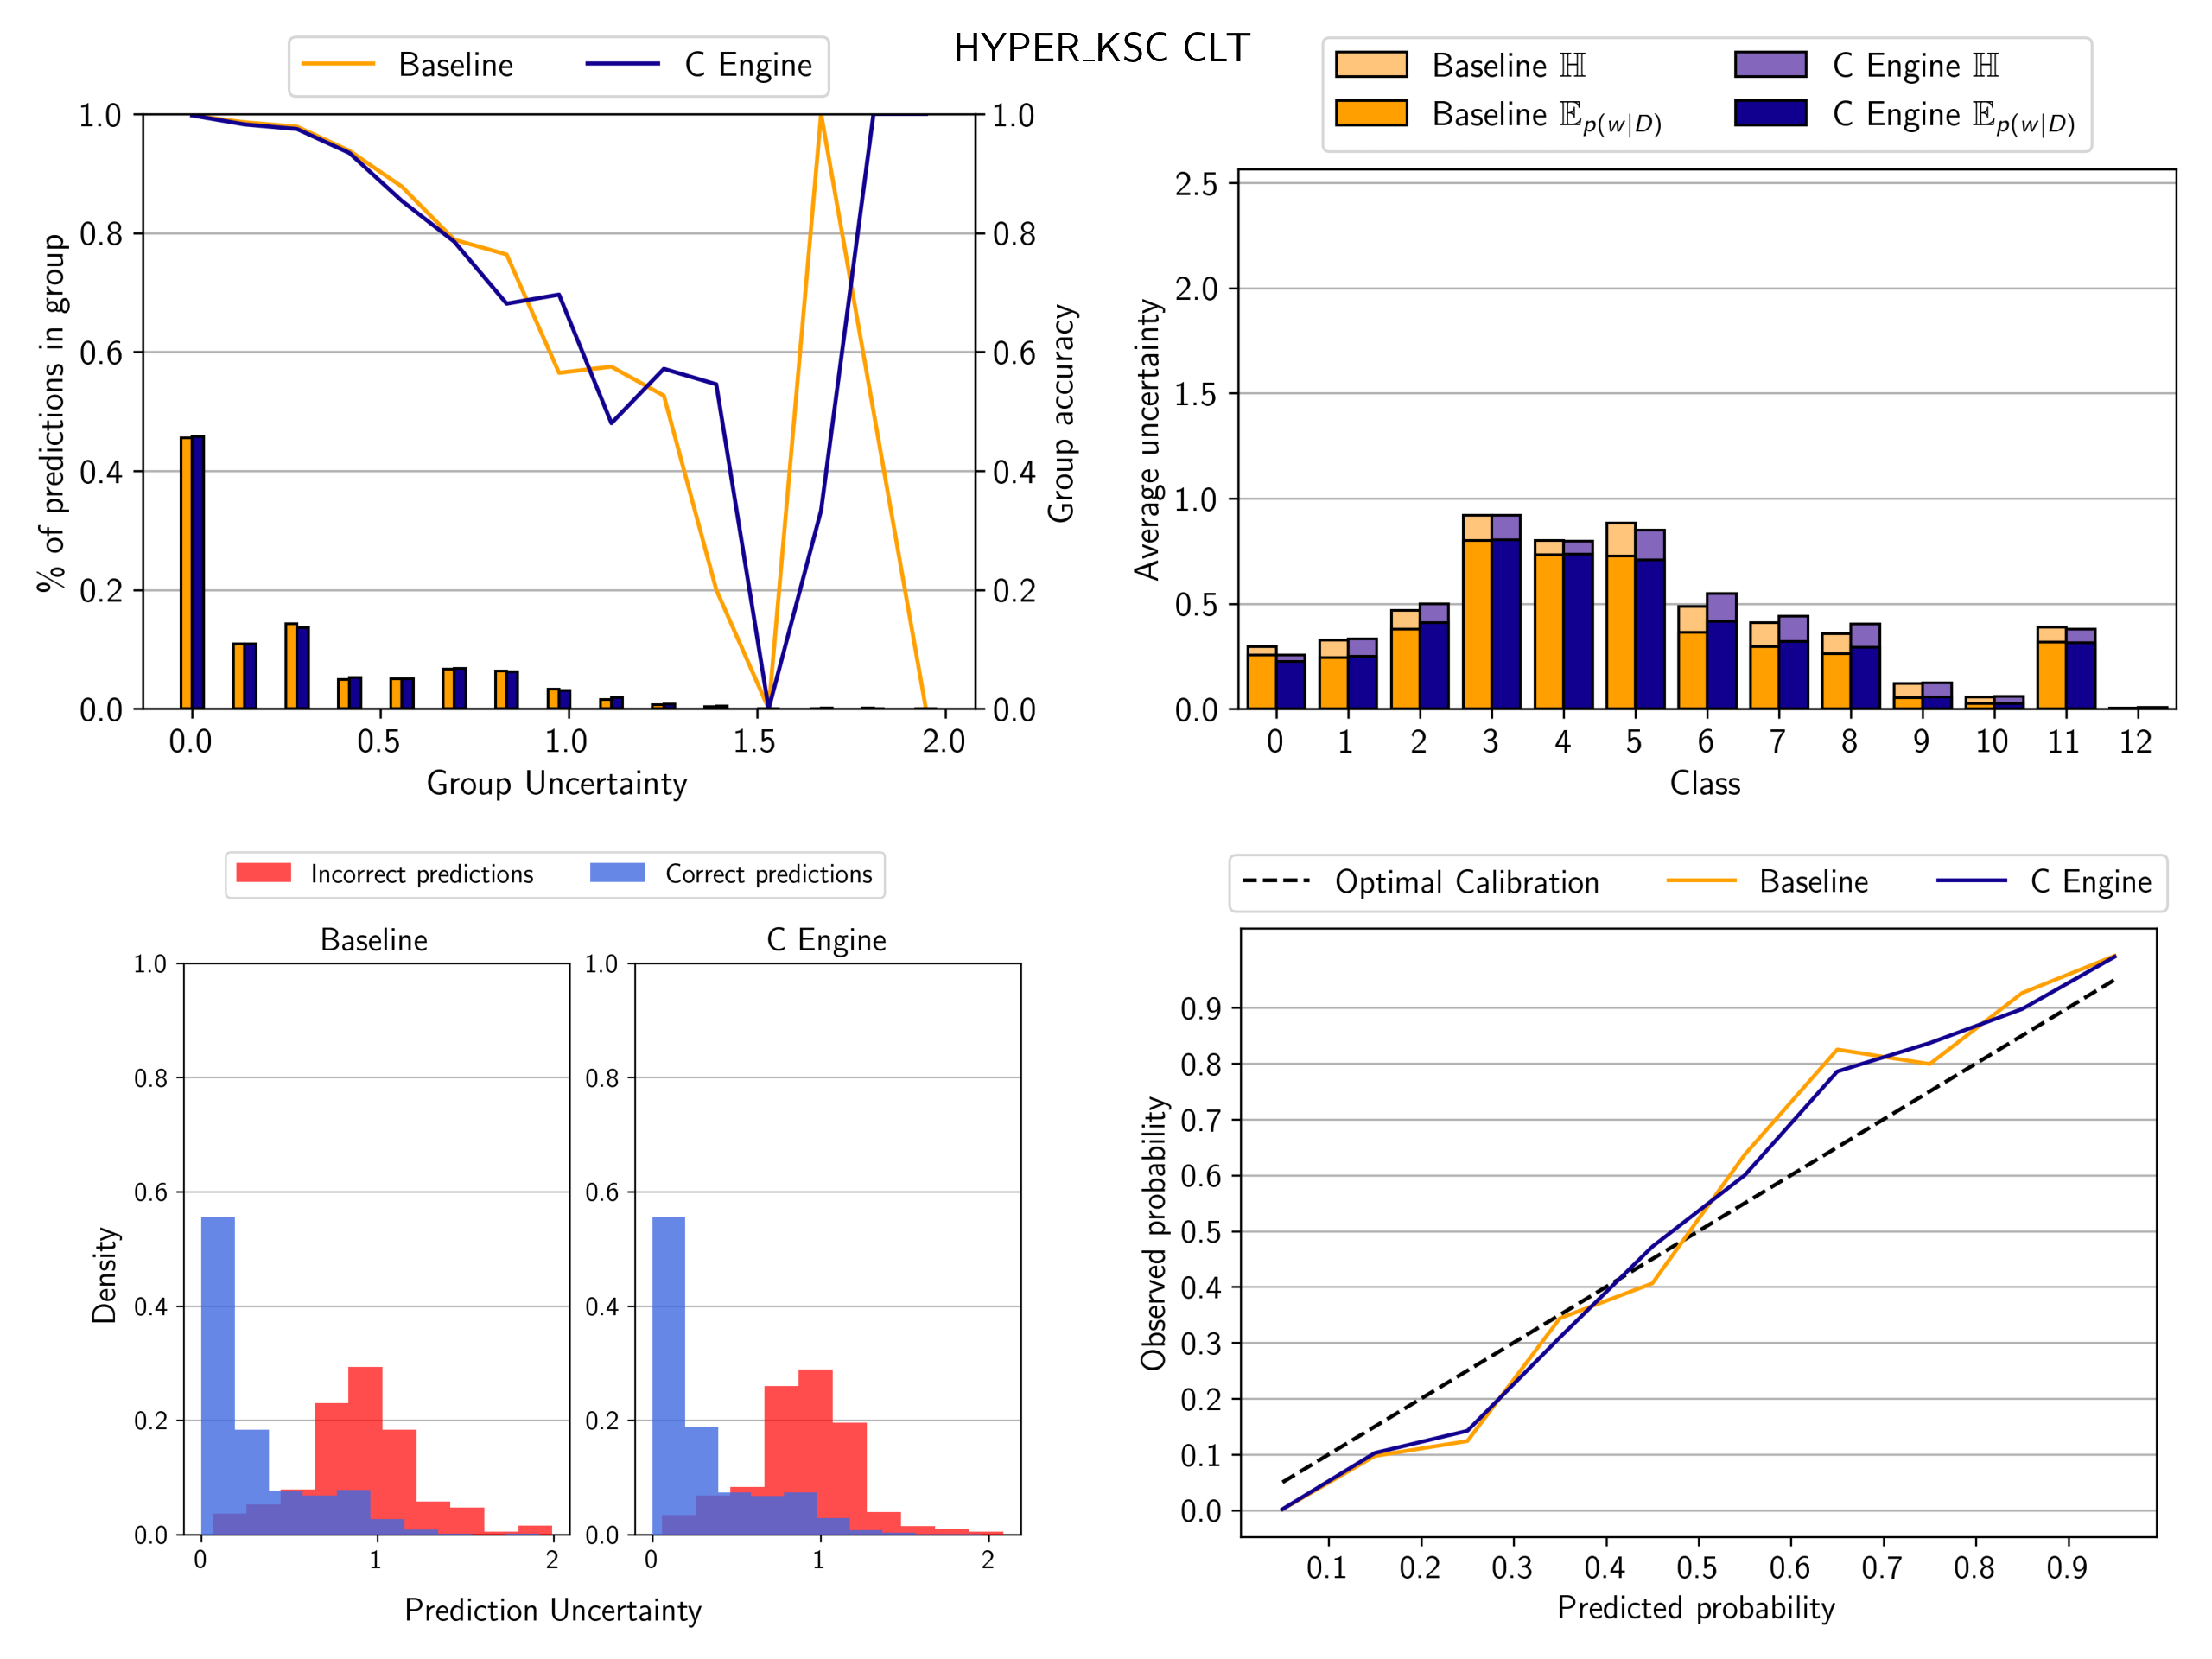
\includegraphics[width=0.9\textwidth]{root/Imagenes/anexo/CLT-HYPER_KSC-mosaic.png}
    \caption{Predicciones del conjunto de prueba de píxeles hiperespectrales KSC.}
    \label{fig:anx-CLT-HYPER_KSC}
\end{figure}


\begin{figure}[ht]
    \centering
    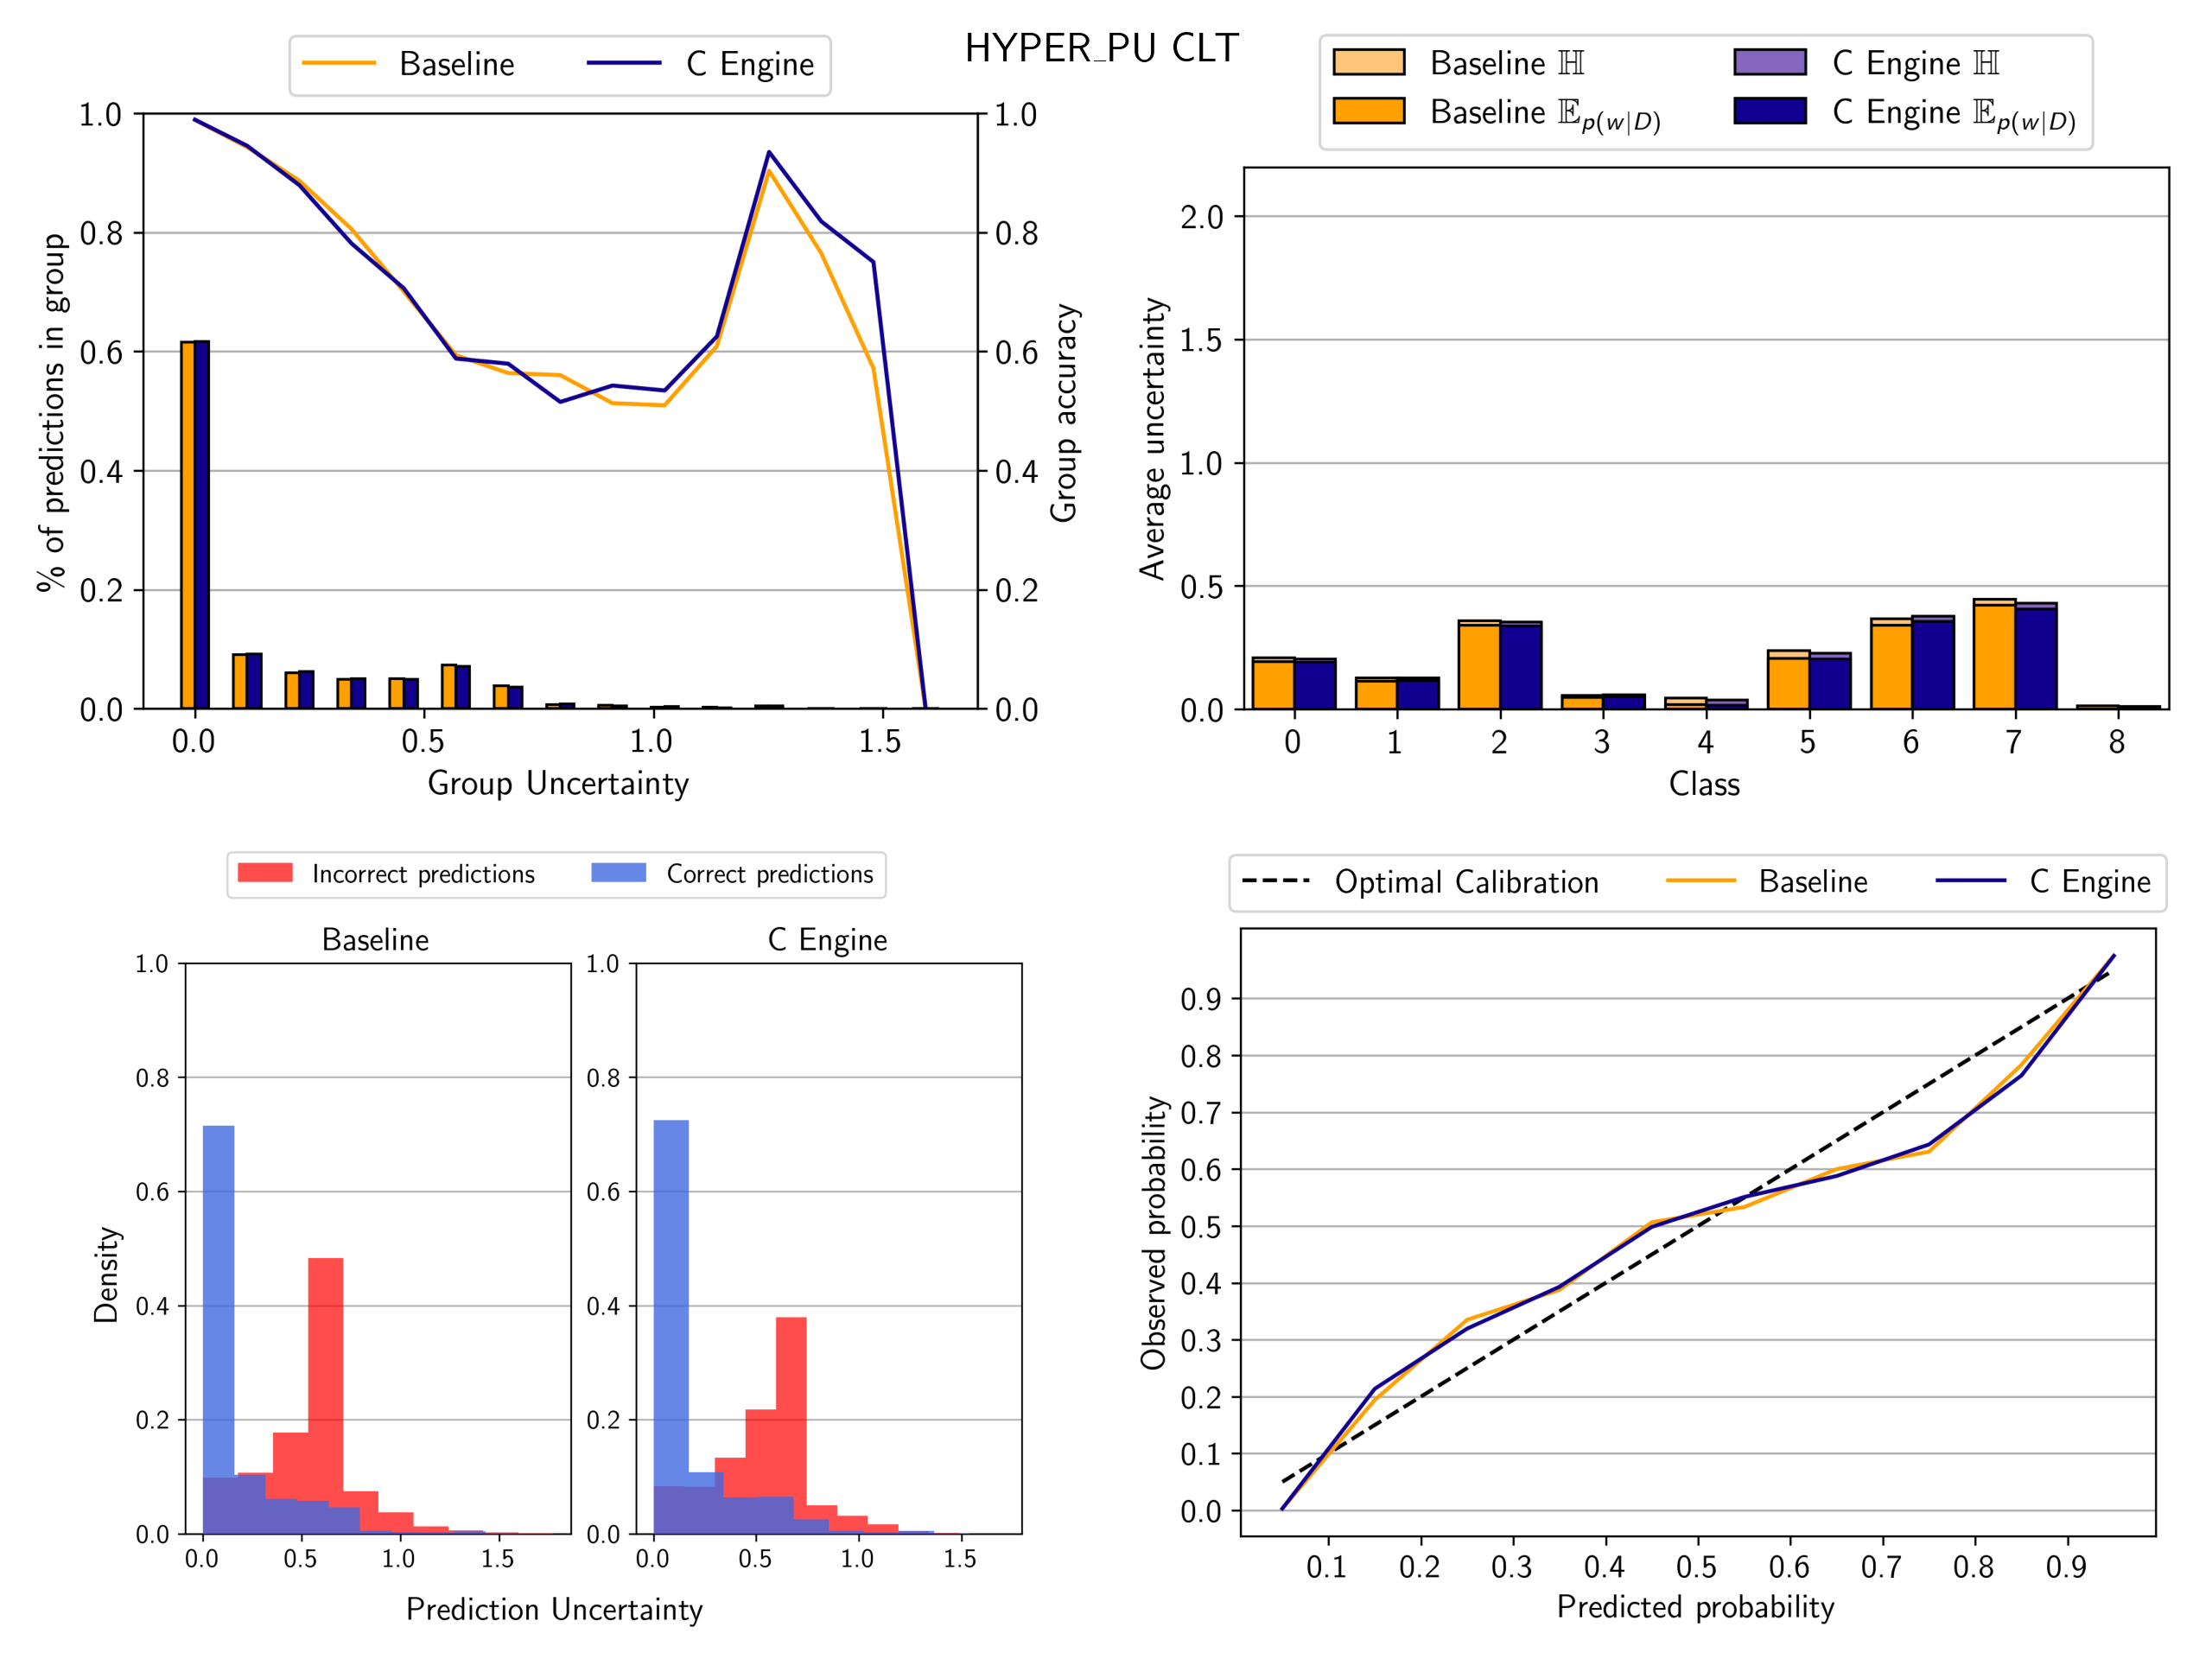
\includegraphics[width=0.9\textwidth]{root/Imagenes/anexo/CLT-HYPER_PU-mosaic.png}
    \caption{Predicciones del conjunto de prueba de píxeles hiperespectrales PU.}
    \label{fig:anx-CLT-HYPER_PU}
\end{figure}


\begin{figure}[ht]
    \centering
    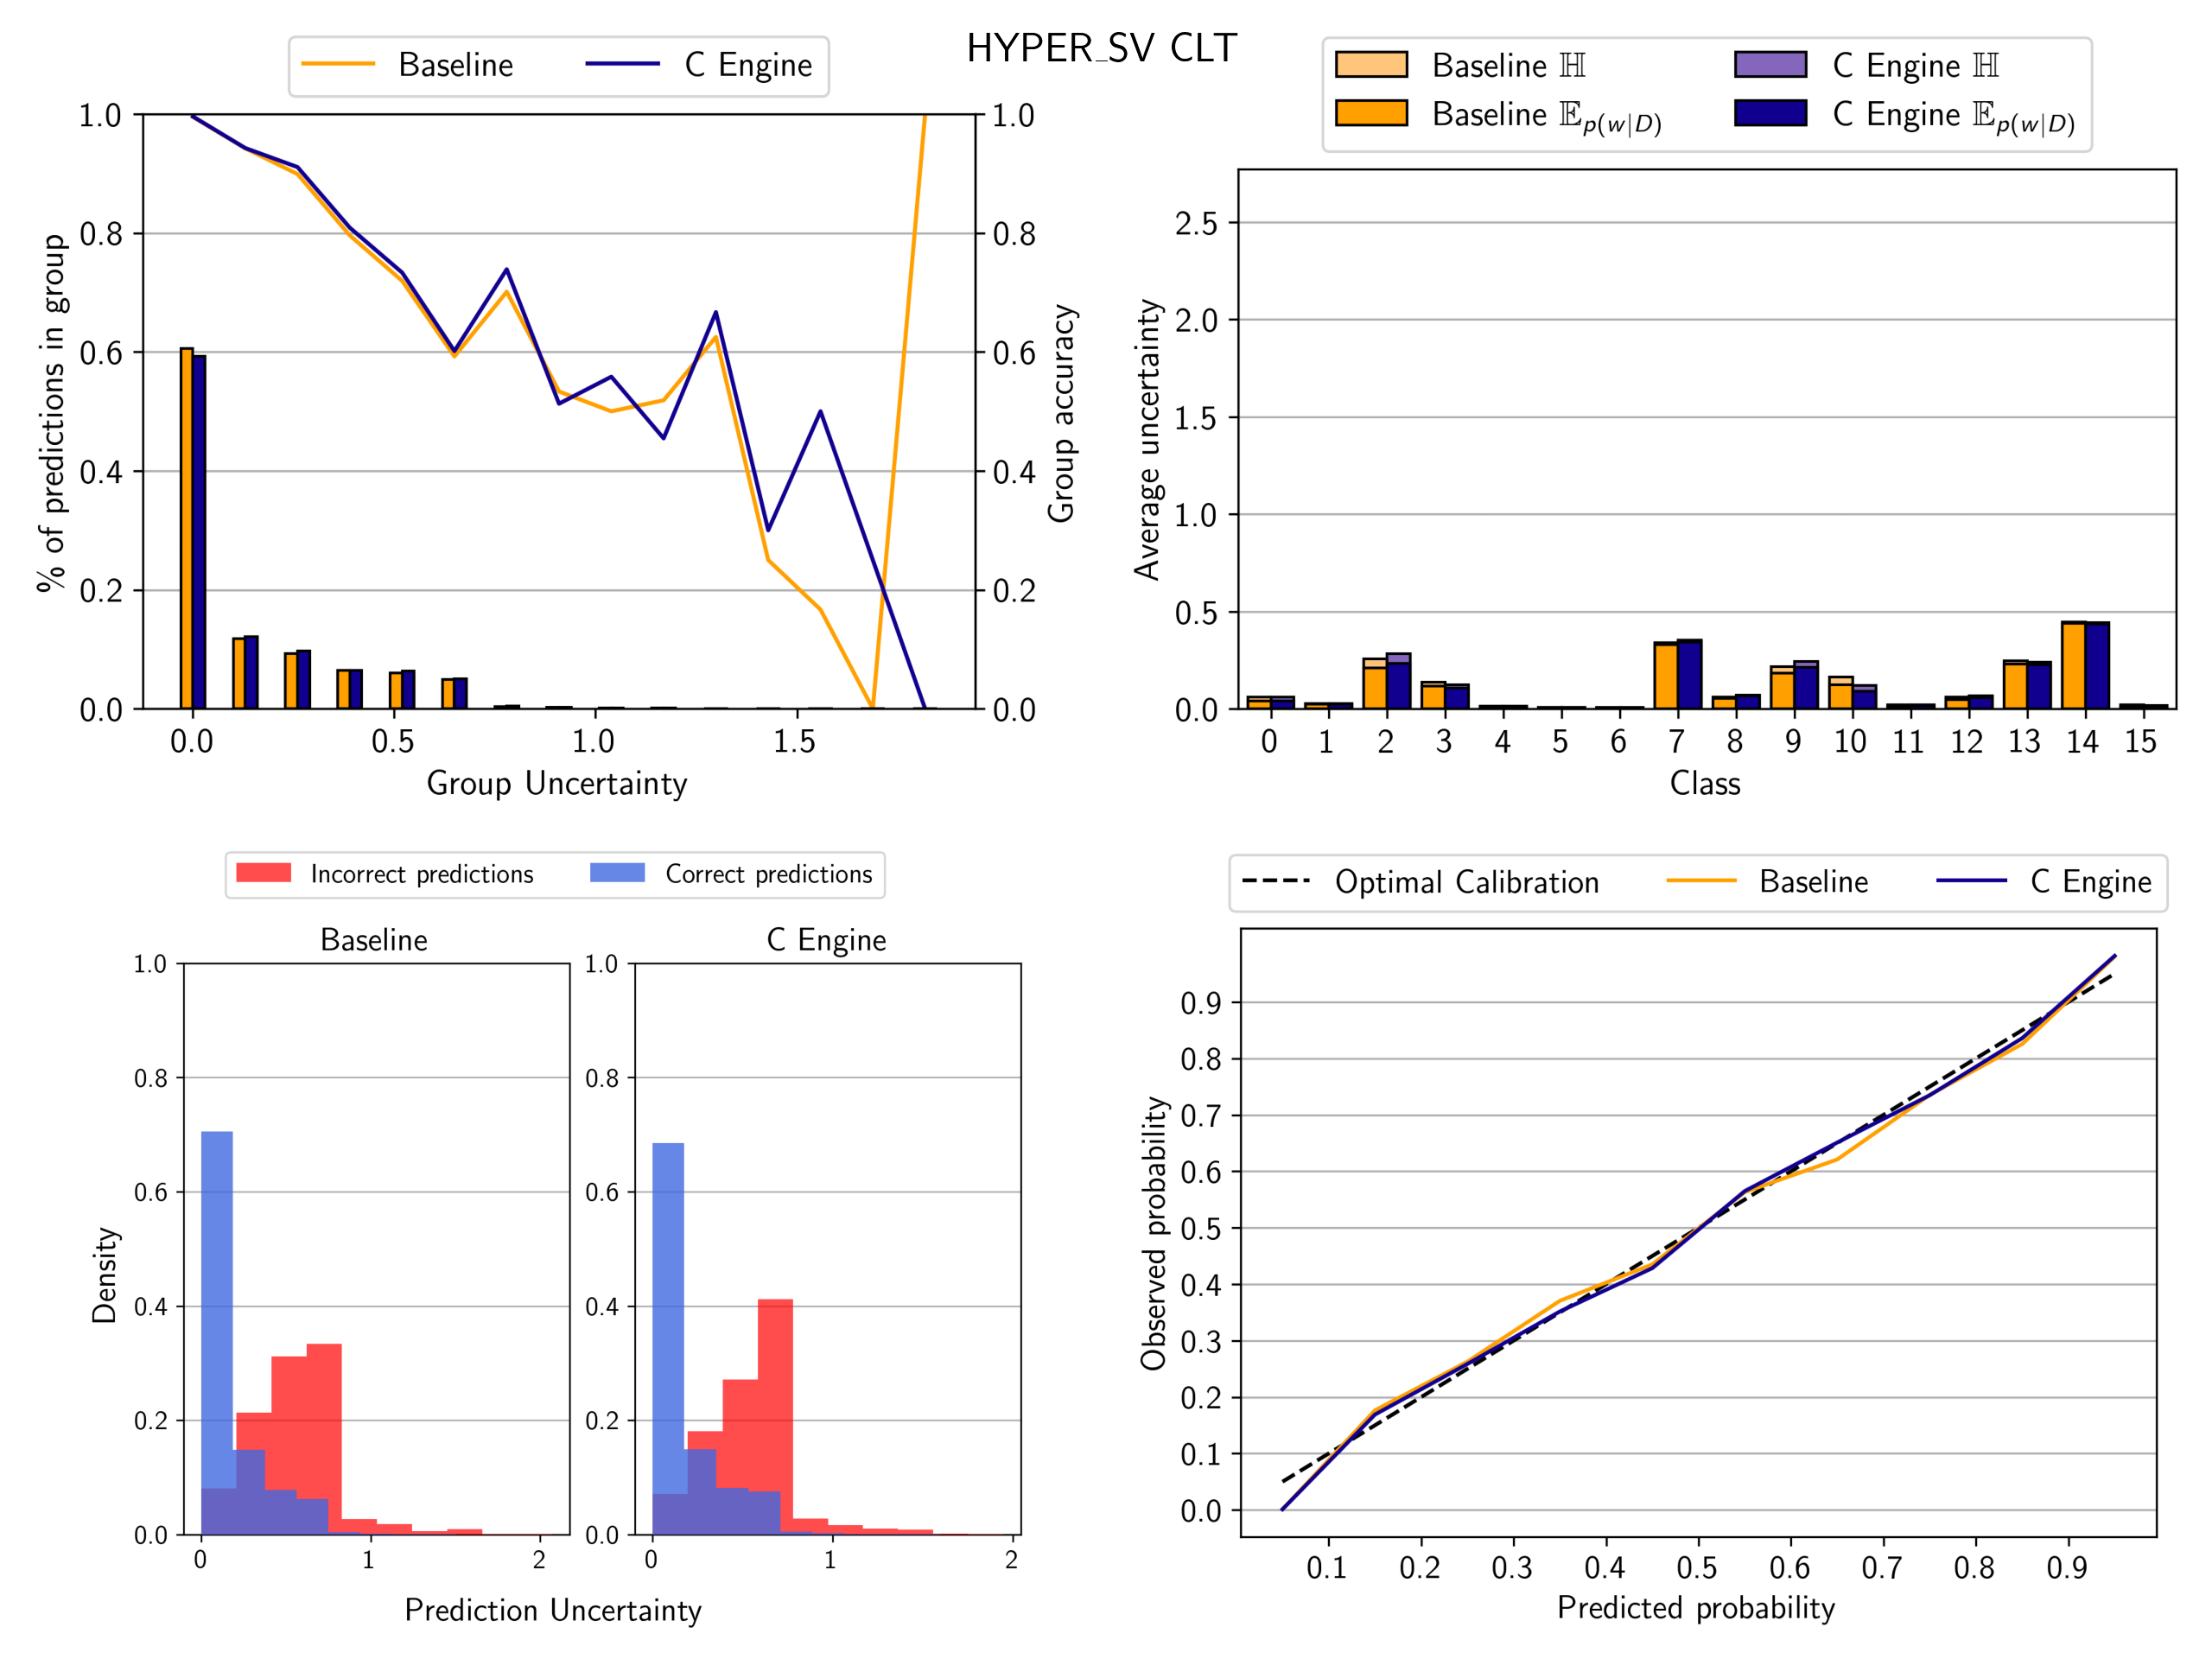
\includegraphics[width=0.9\textwidth]{root/Imagenes/anexo/CLT-HYPER_SV-mosaic.png}
    \caption{Predicciones del conjunto de prueba de píxeles hiperespectrales SV.}
    \label{fig:anx-CLT-HYPER_SV}
\end{figure}


\begin{figure}[ht]
    \centering
    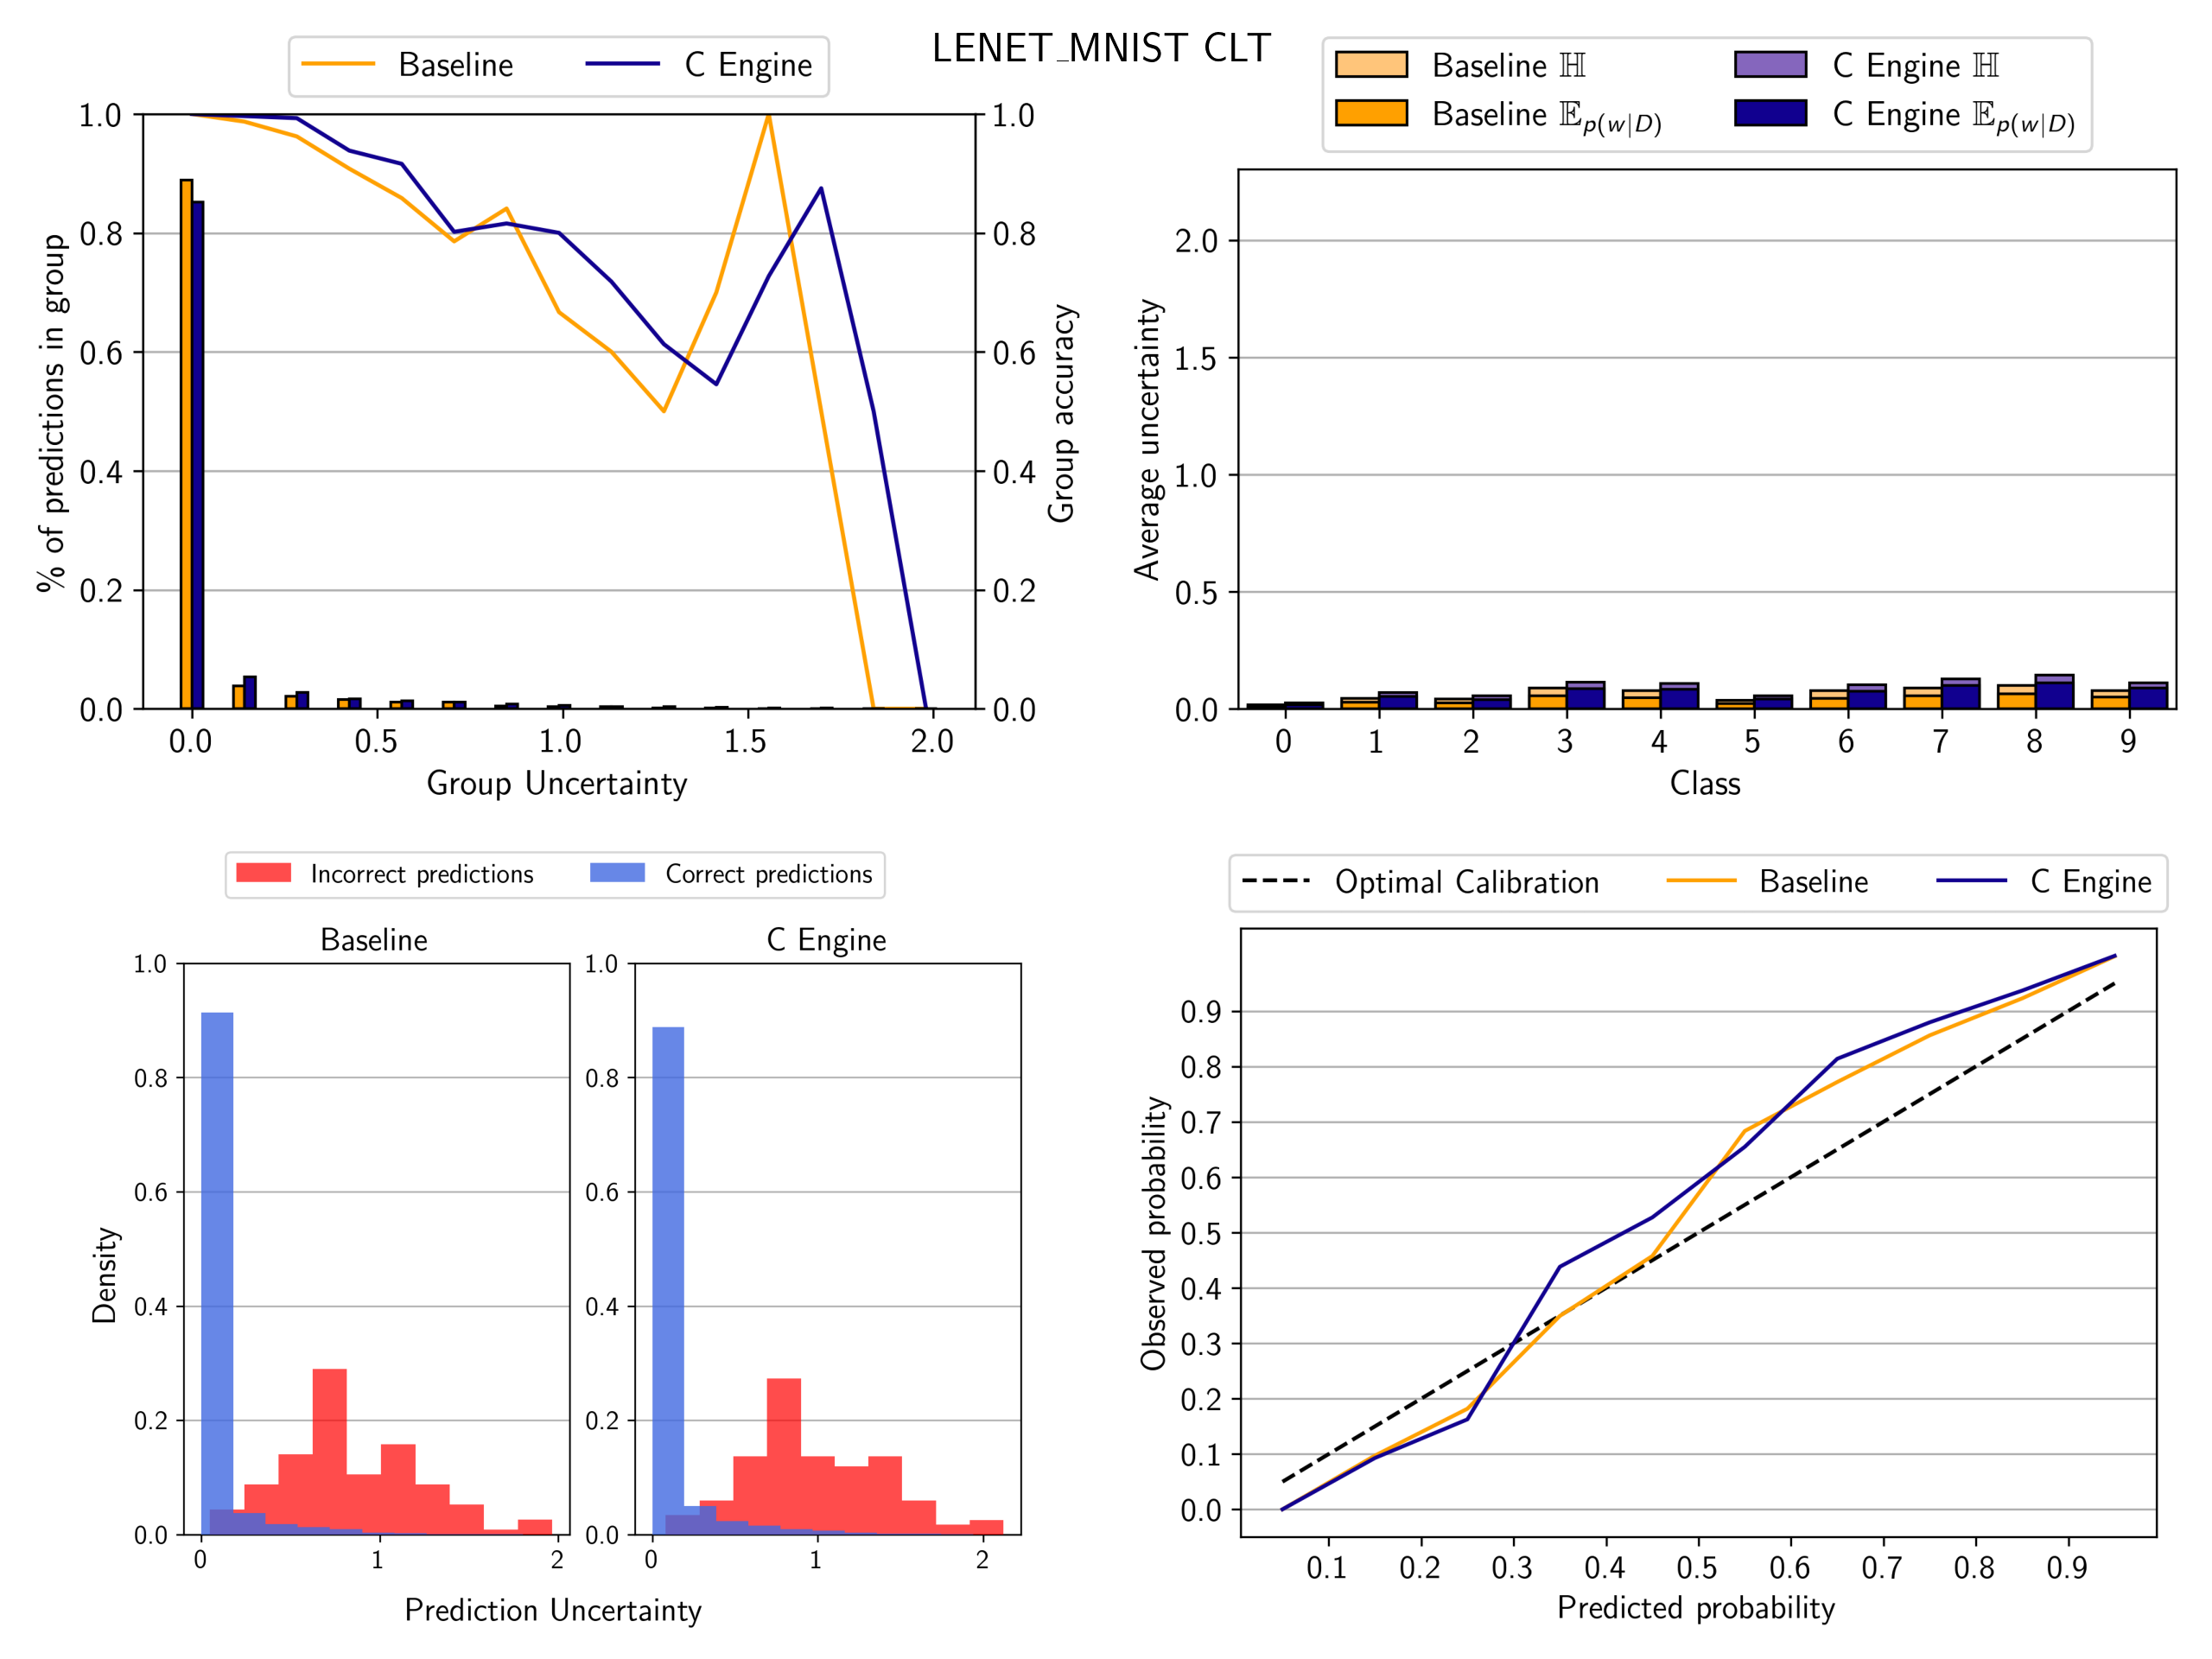
\includegraphics[width=0.9\textwidth]{root/Imagenes/anexo/CLT-LENET_MNIST-mosaic.png}
    \caption{Predicciones del modelo LENET con el conjunto de datos MNIST.}
    \label{fig:anx-CLT-LENET_MNIST}
\end{figure}


\begin{figure}[ht]
    \centering
    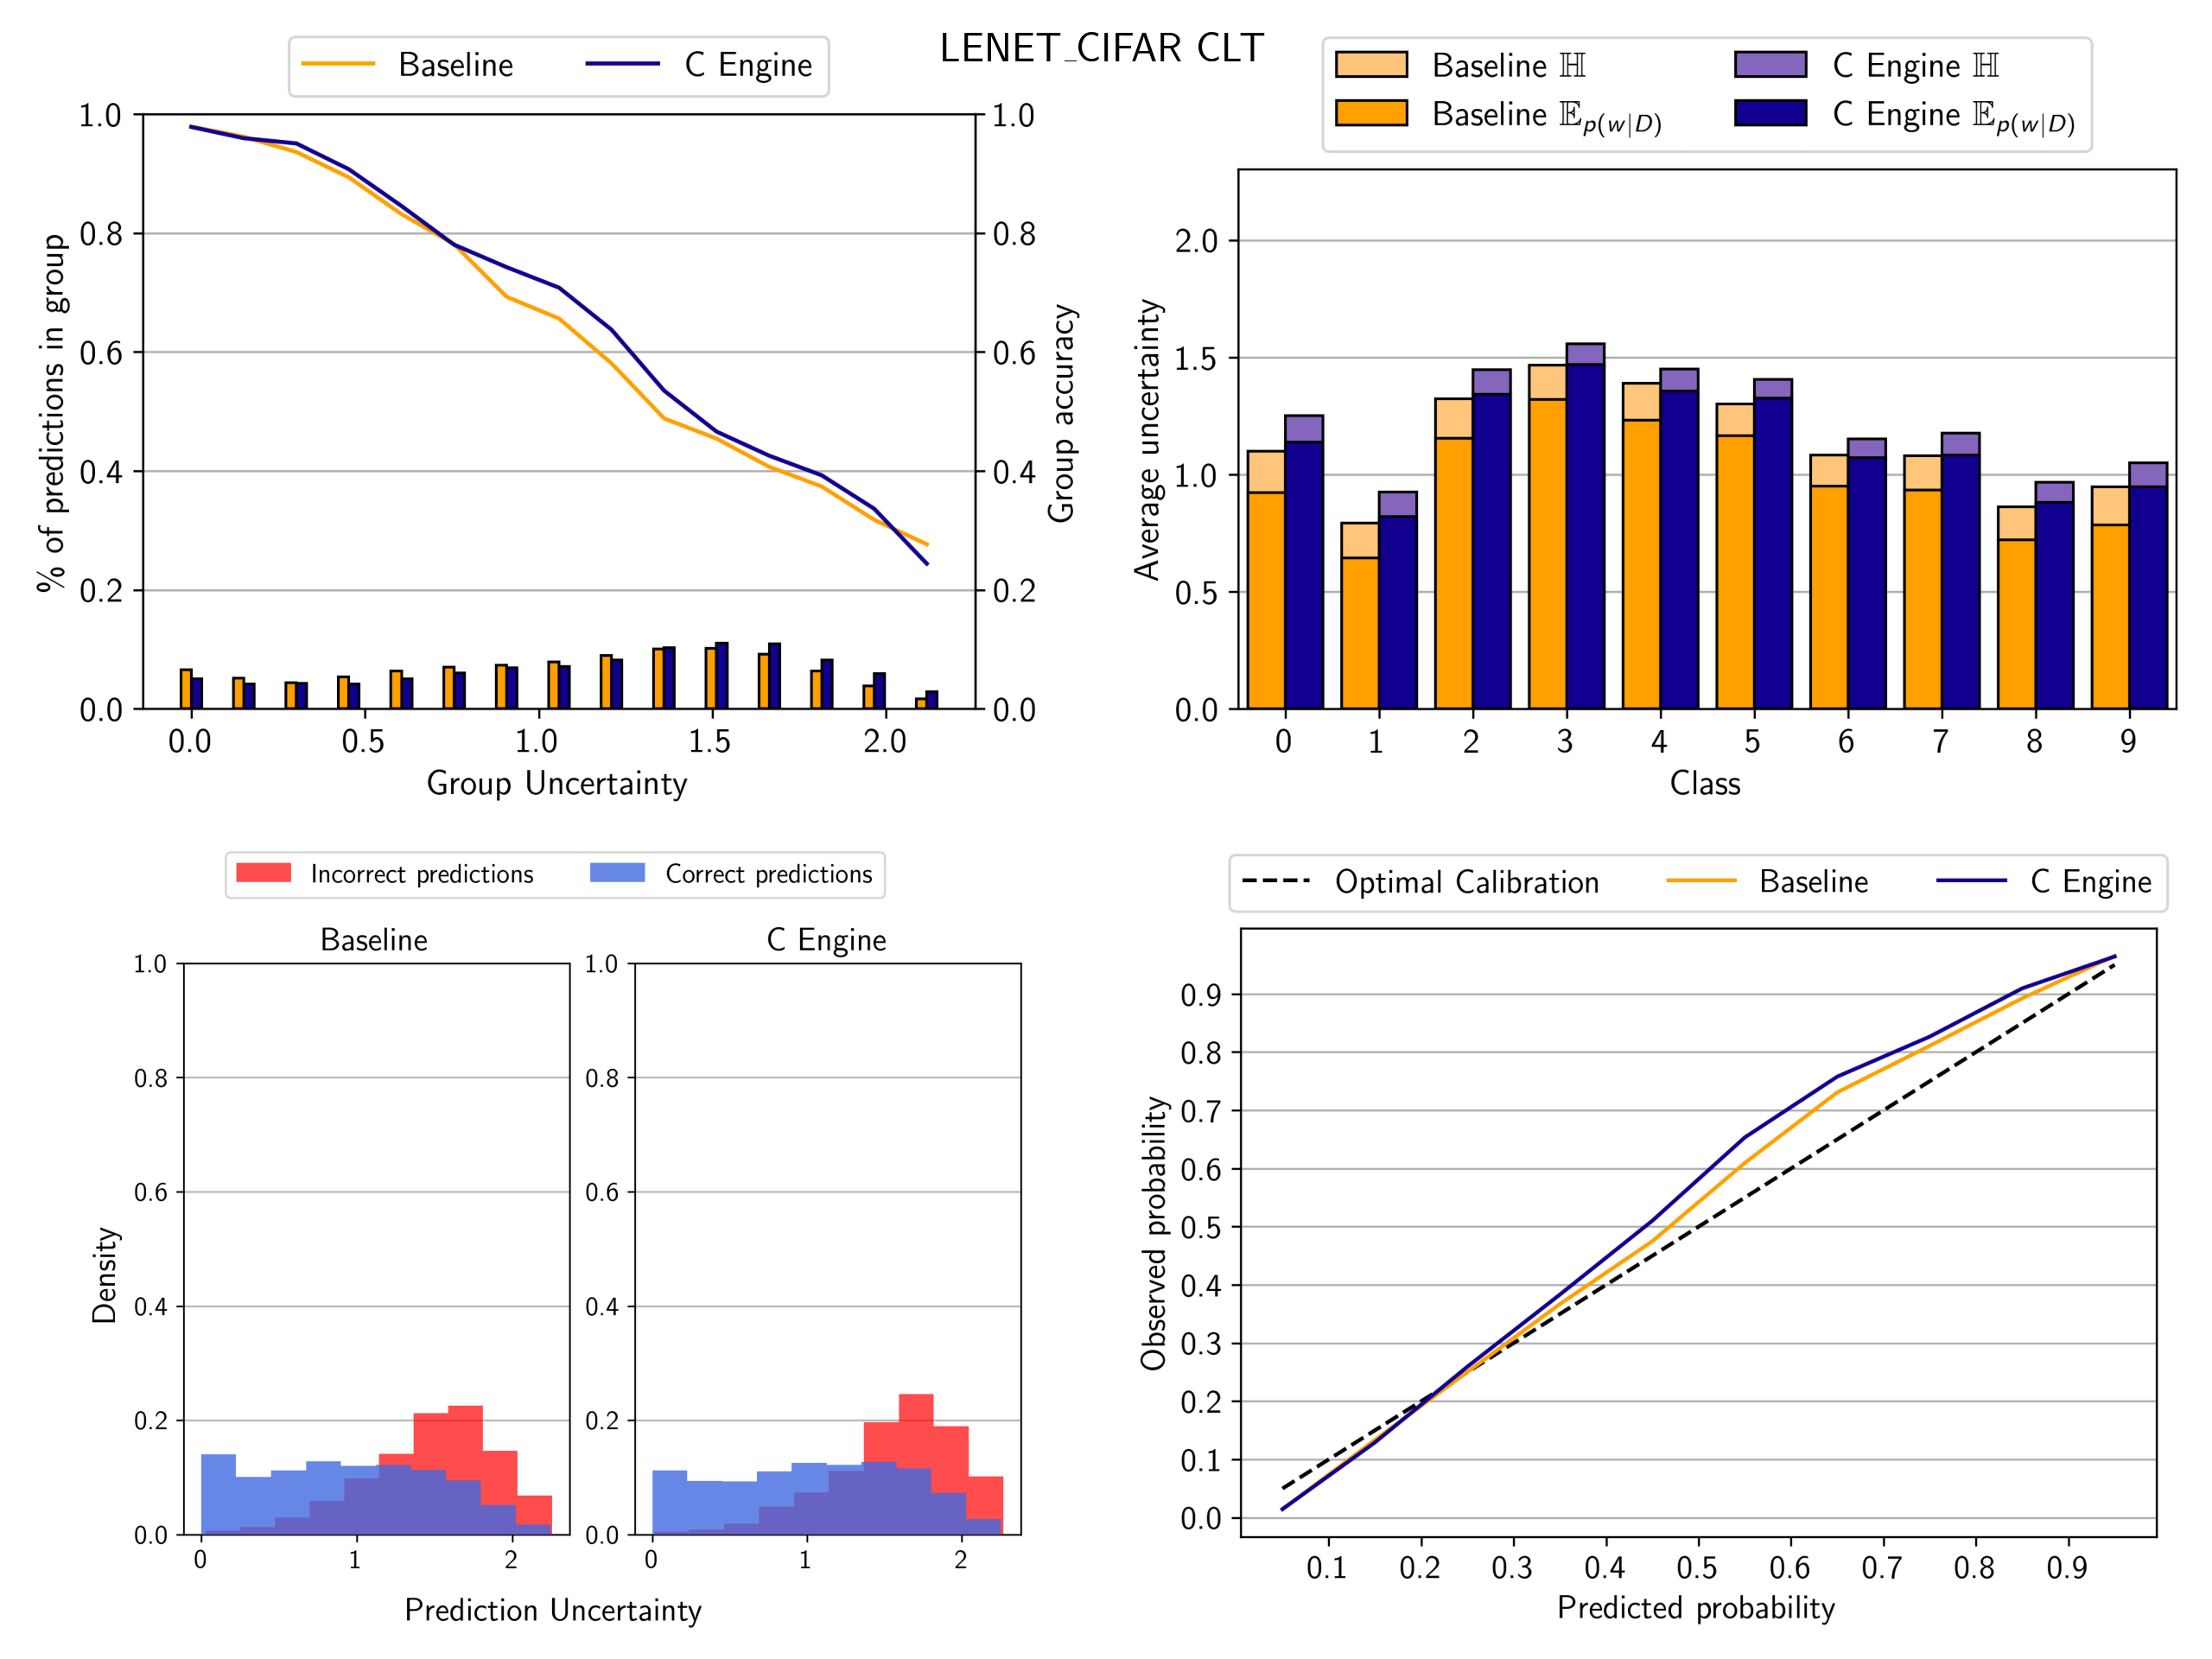
\includegraphics[width=0.9\textwidth]{root/Imagenes/anexo/CLT-LENET_CIFAR-mosaic.png}
    \caption{Predicciones del modelo LENET con el conjunto de datos CIFAR-10.}
    \label{fig:anx-CLT-LENET_CIFAR}
\end{figure}


\begin{figure}[ht]
    \centering
    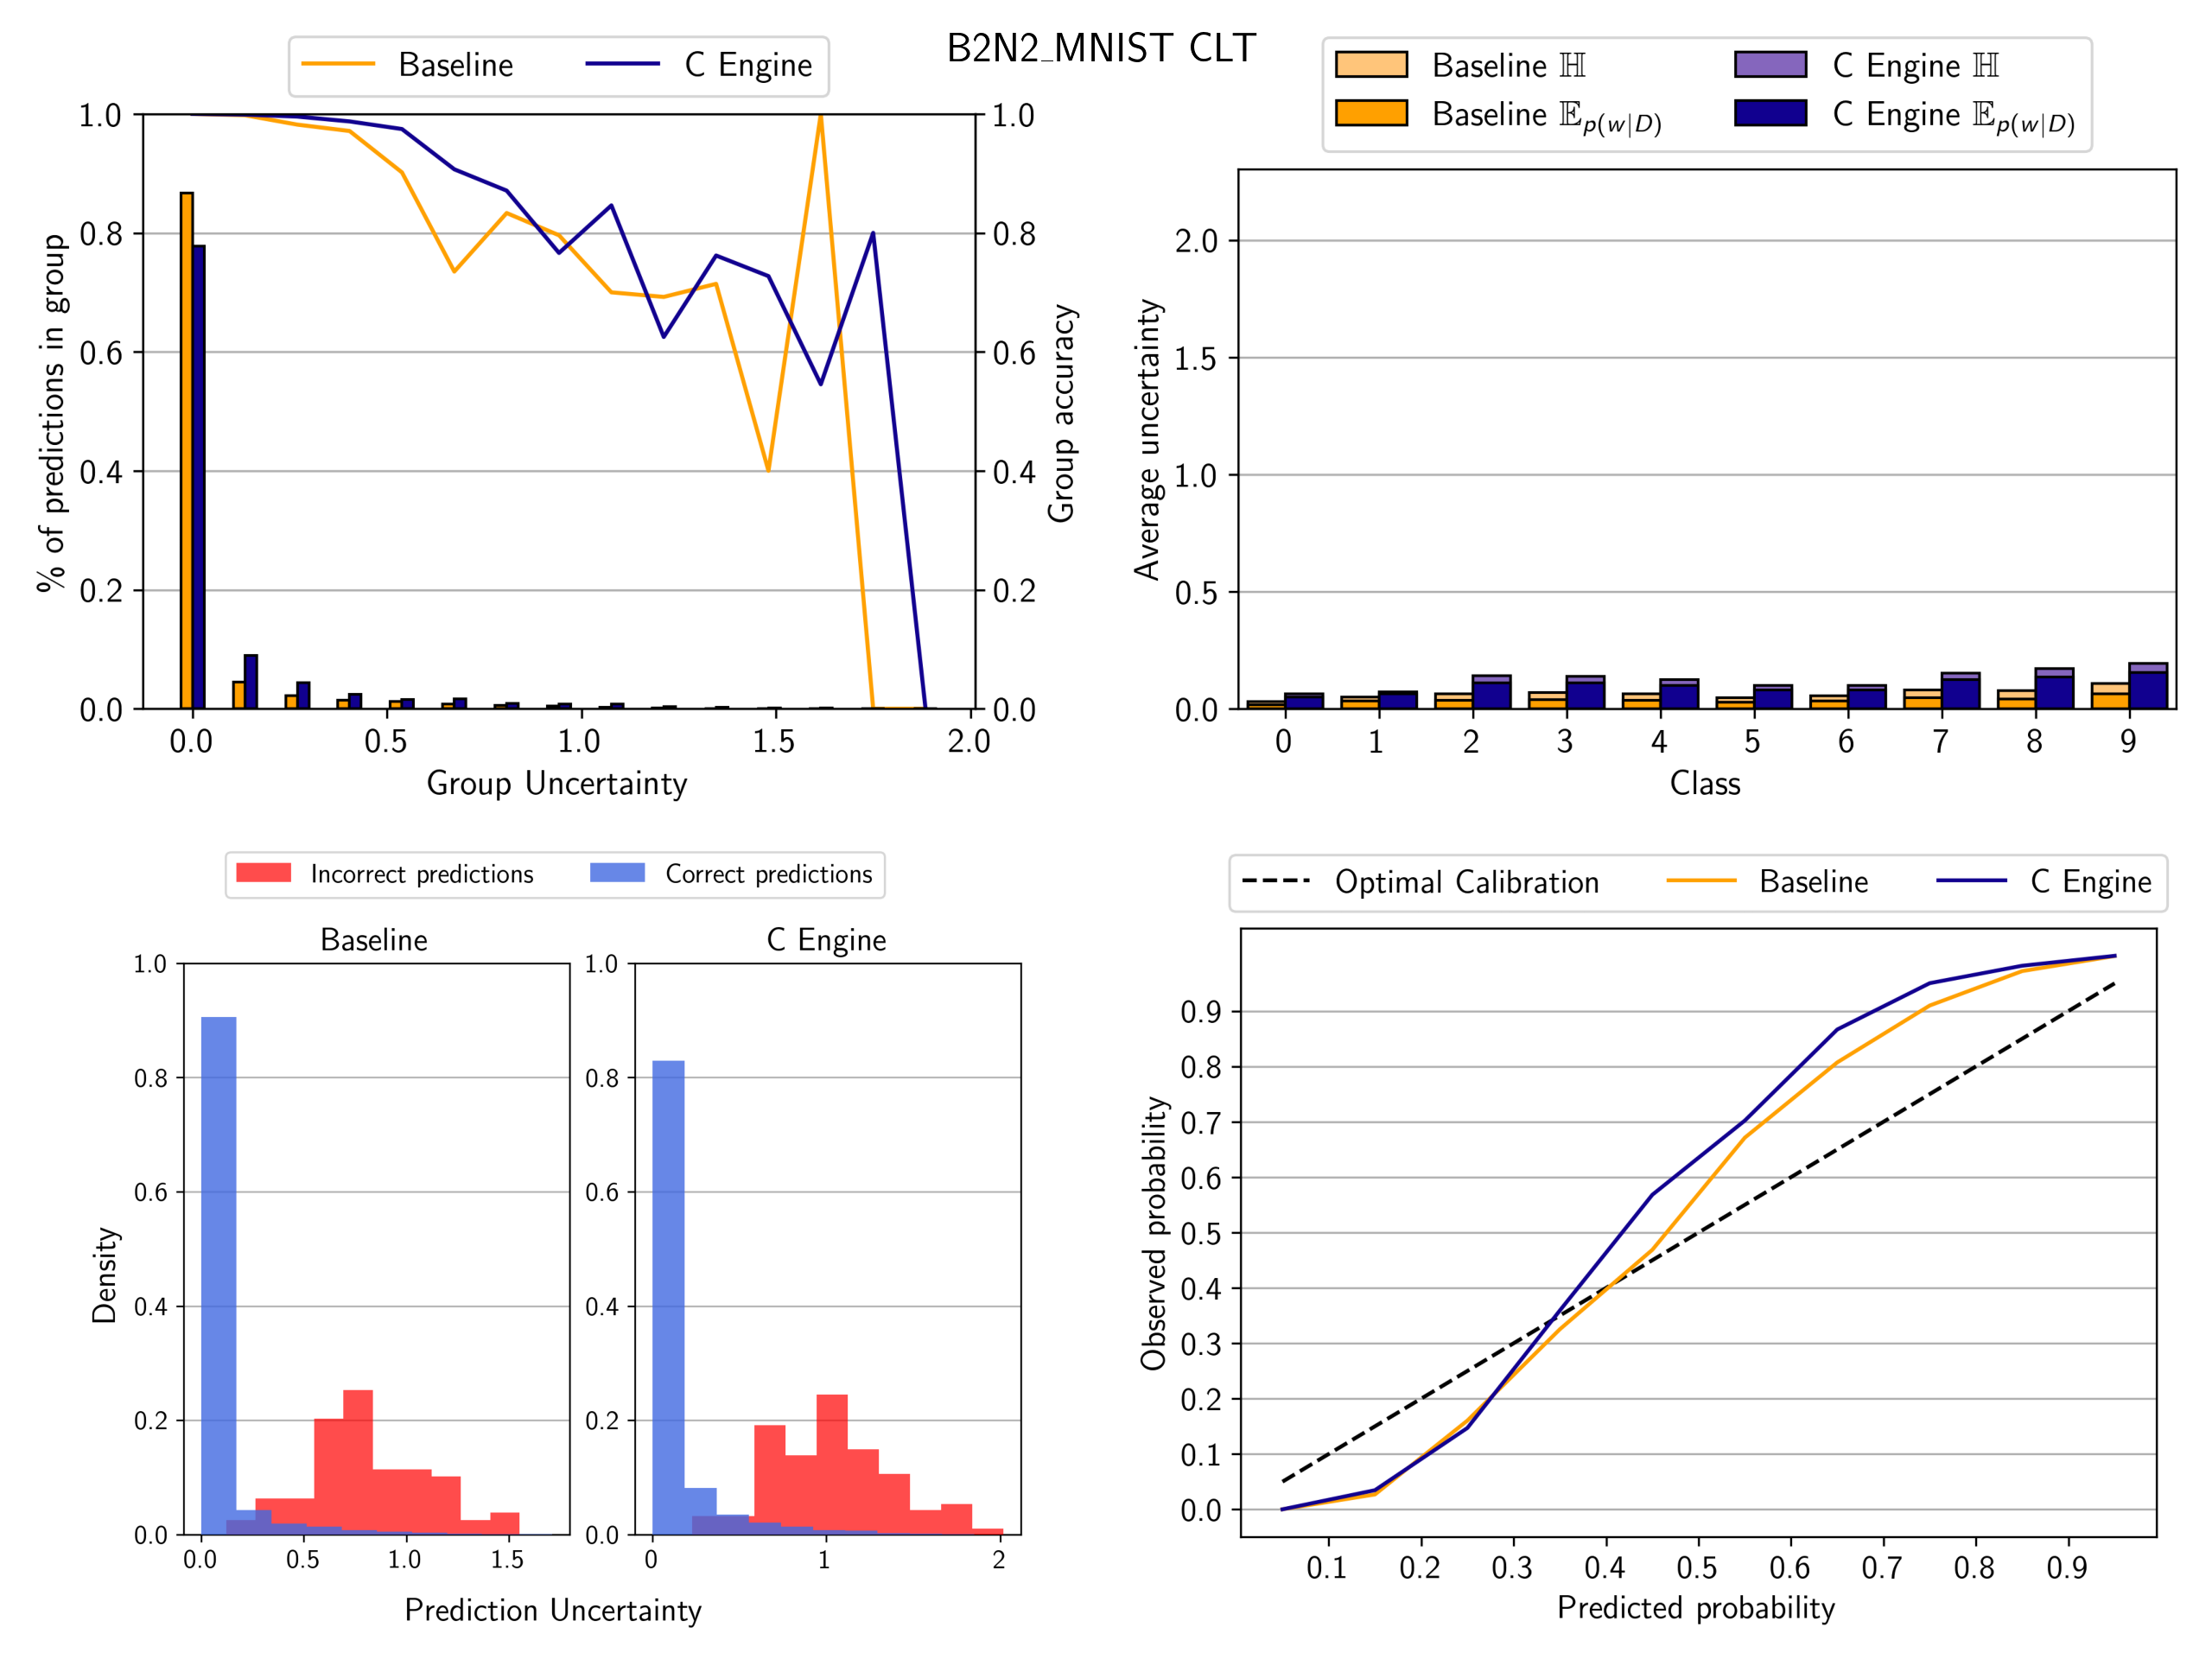
\includegraphics[width=0.9\textwidth]{root/Imagenes/anexo/CLT-B2N2_MNIST-mosaic.png}
    \caption{Predicciones del modelo B2N2 con el conjunto de datos MNIST.}
    \label{fig:anx-CLT-B2N2_MNIST}
\end{figure}


\begin{figure}[ht]
    \centering
    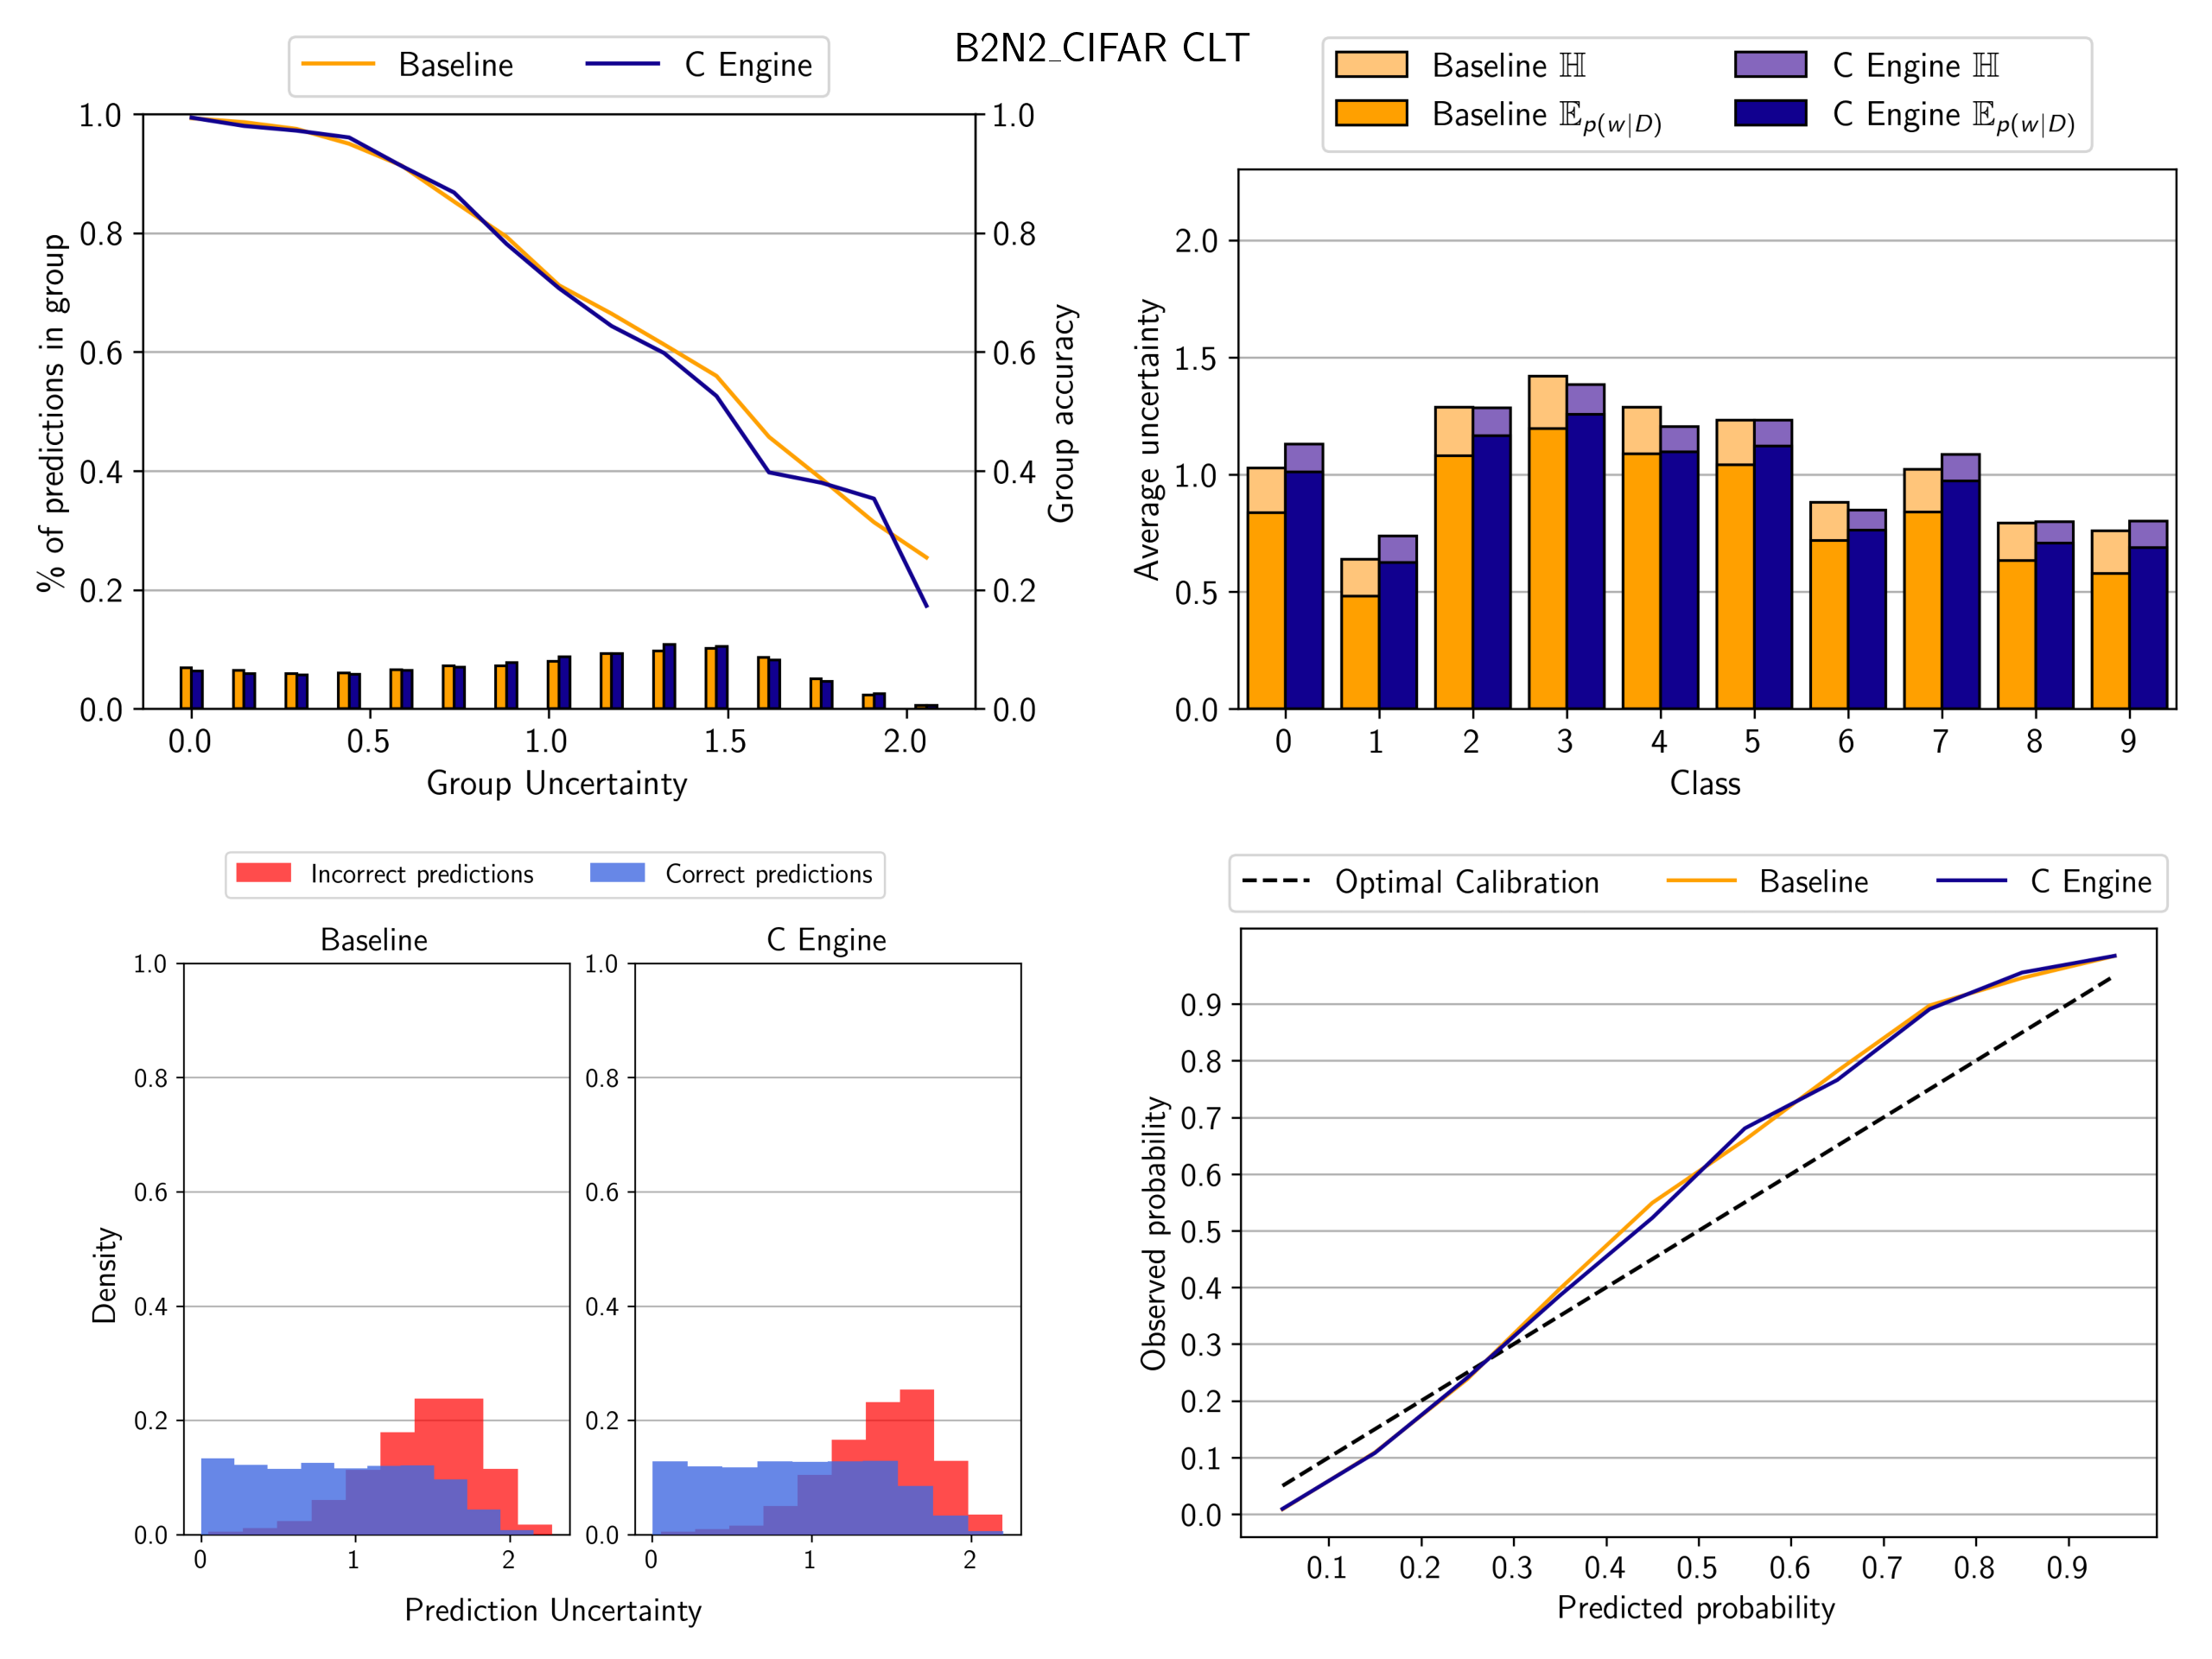
\includegraphics[width=0.9\textwidth]{root/Imagenes/anexo/CLT-B2N2_CIFAR-mosaic.png}
    \caption{Predicciones del modelo B2N2 con el conjunto de datos CIFAR-10.}
    \label{fig:anx-CLT-B2N2_CIFAR}
\end{figure}


\chapter{Resultados de incertidumbre optimización Bernoulli} \label{anx:bernoulli}

\begin{figure}[ht]
    \centering
    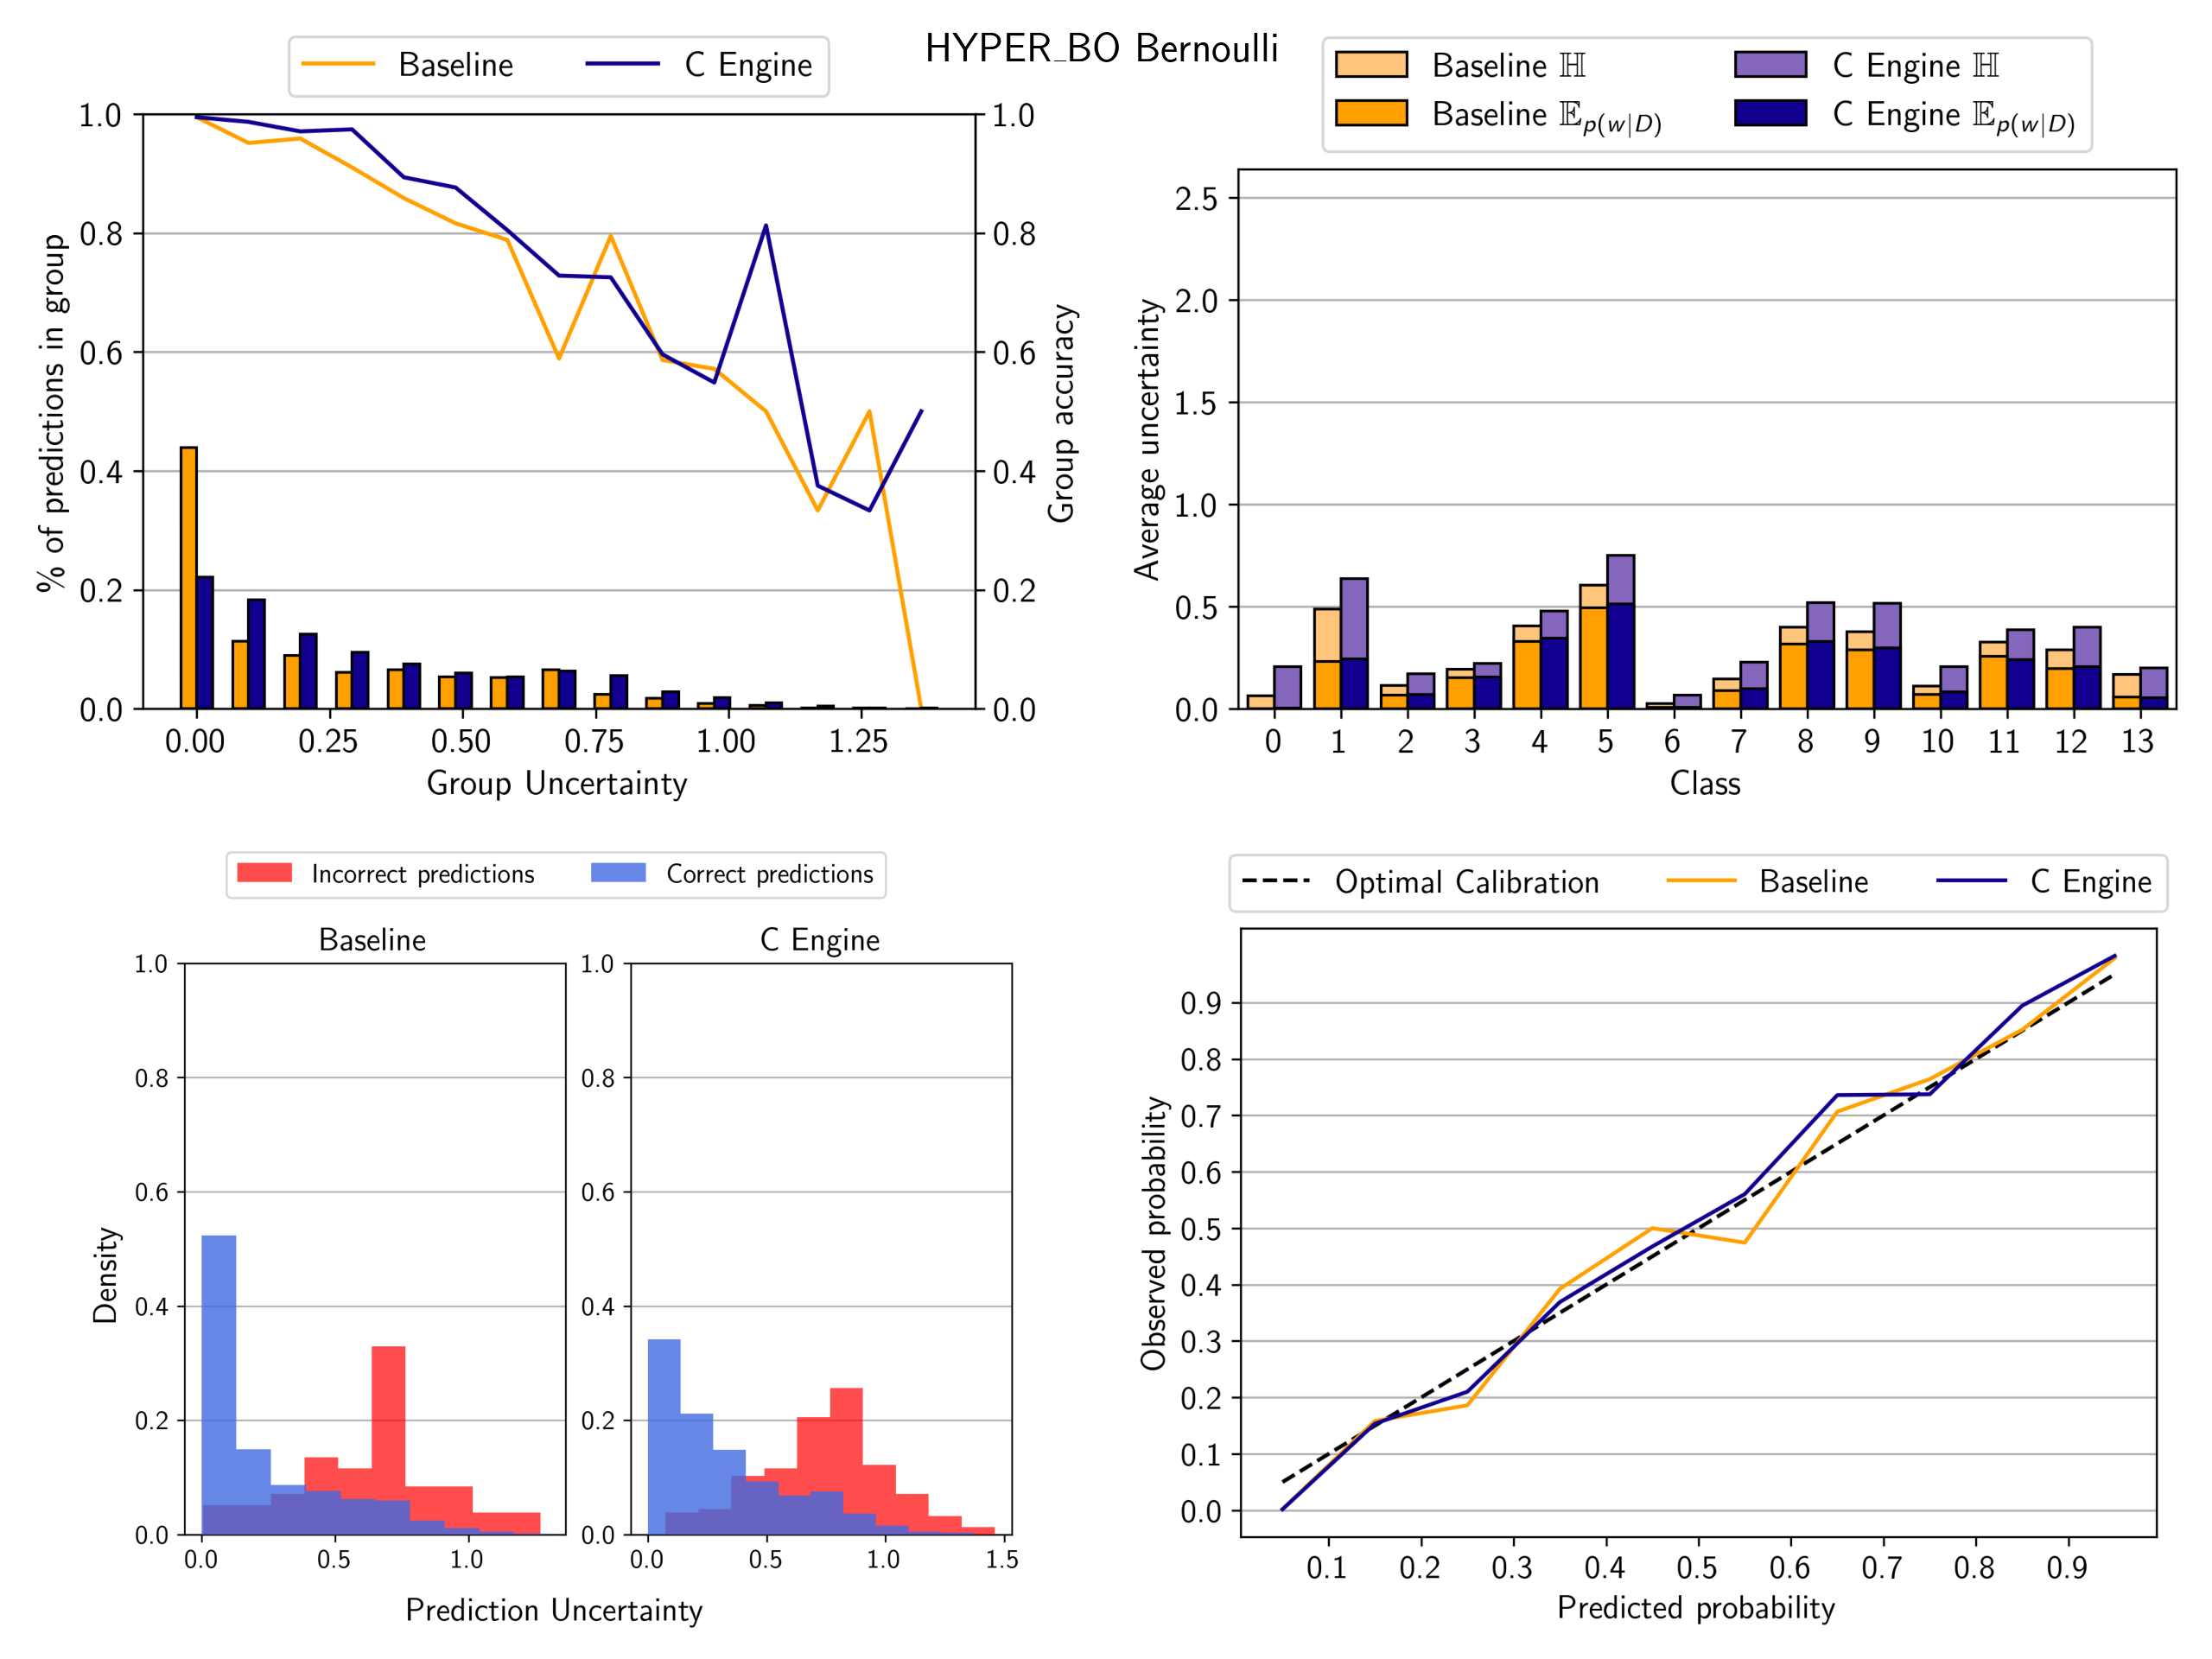
\includegraphics[width=0.9\textwidth]{root/Imagenes/anexo/Bernoulli-HYPER_BO-mosaic.png}
    \caption{Predicciones del conjunto de prueba de píxeles hiperespectrales BO.}
    \label{fig:anx-Bernoulli-HYPER_BO}
\end{figure}


\begin{figure}[ht]
    \centering
    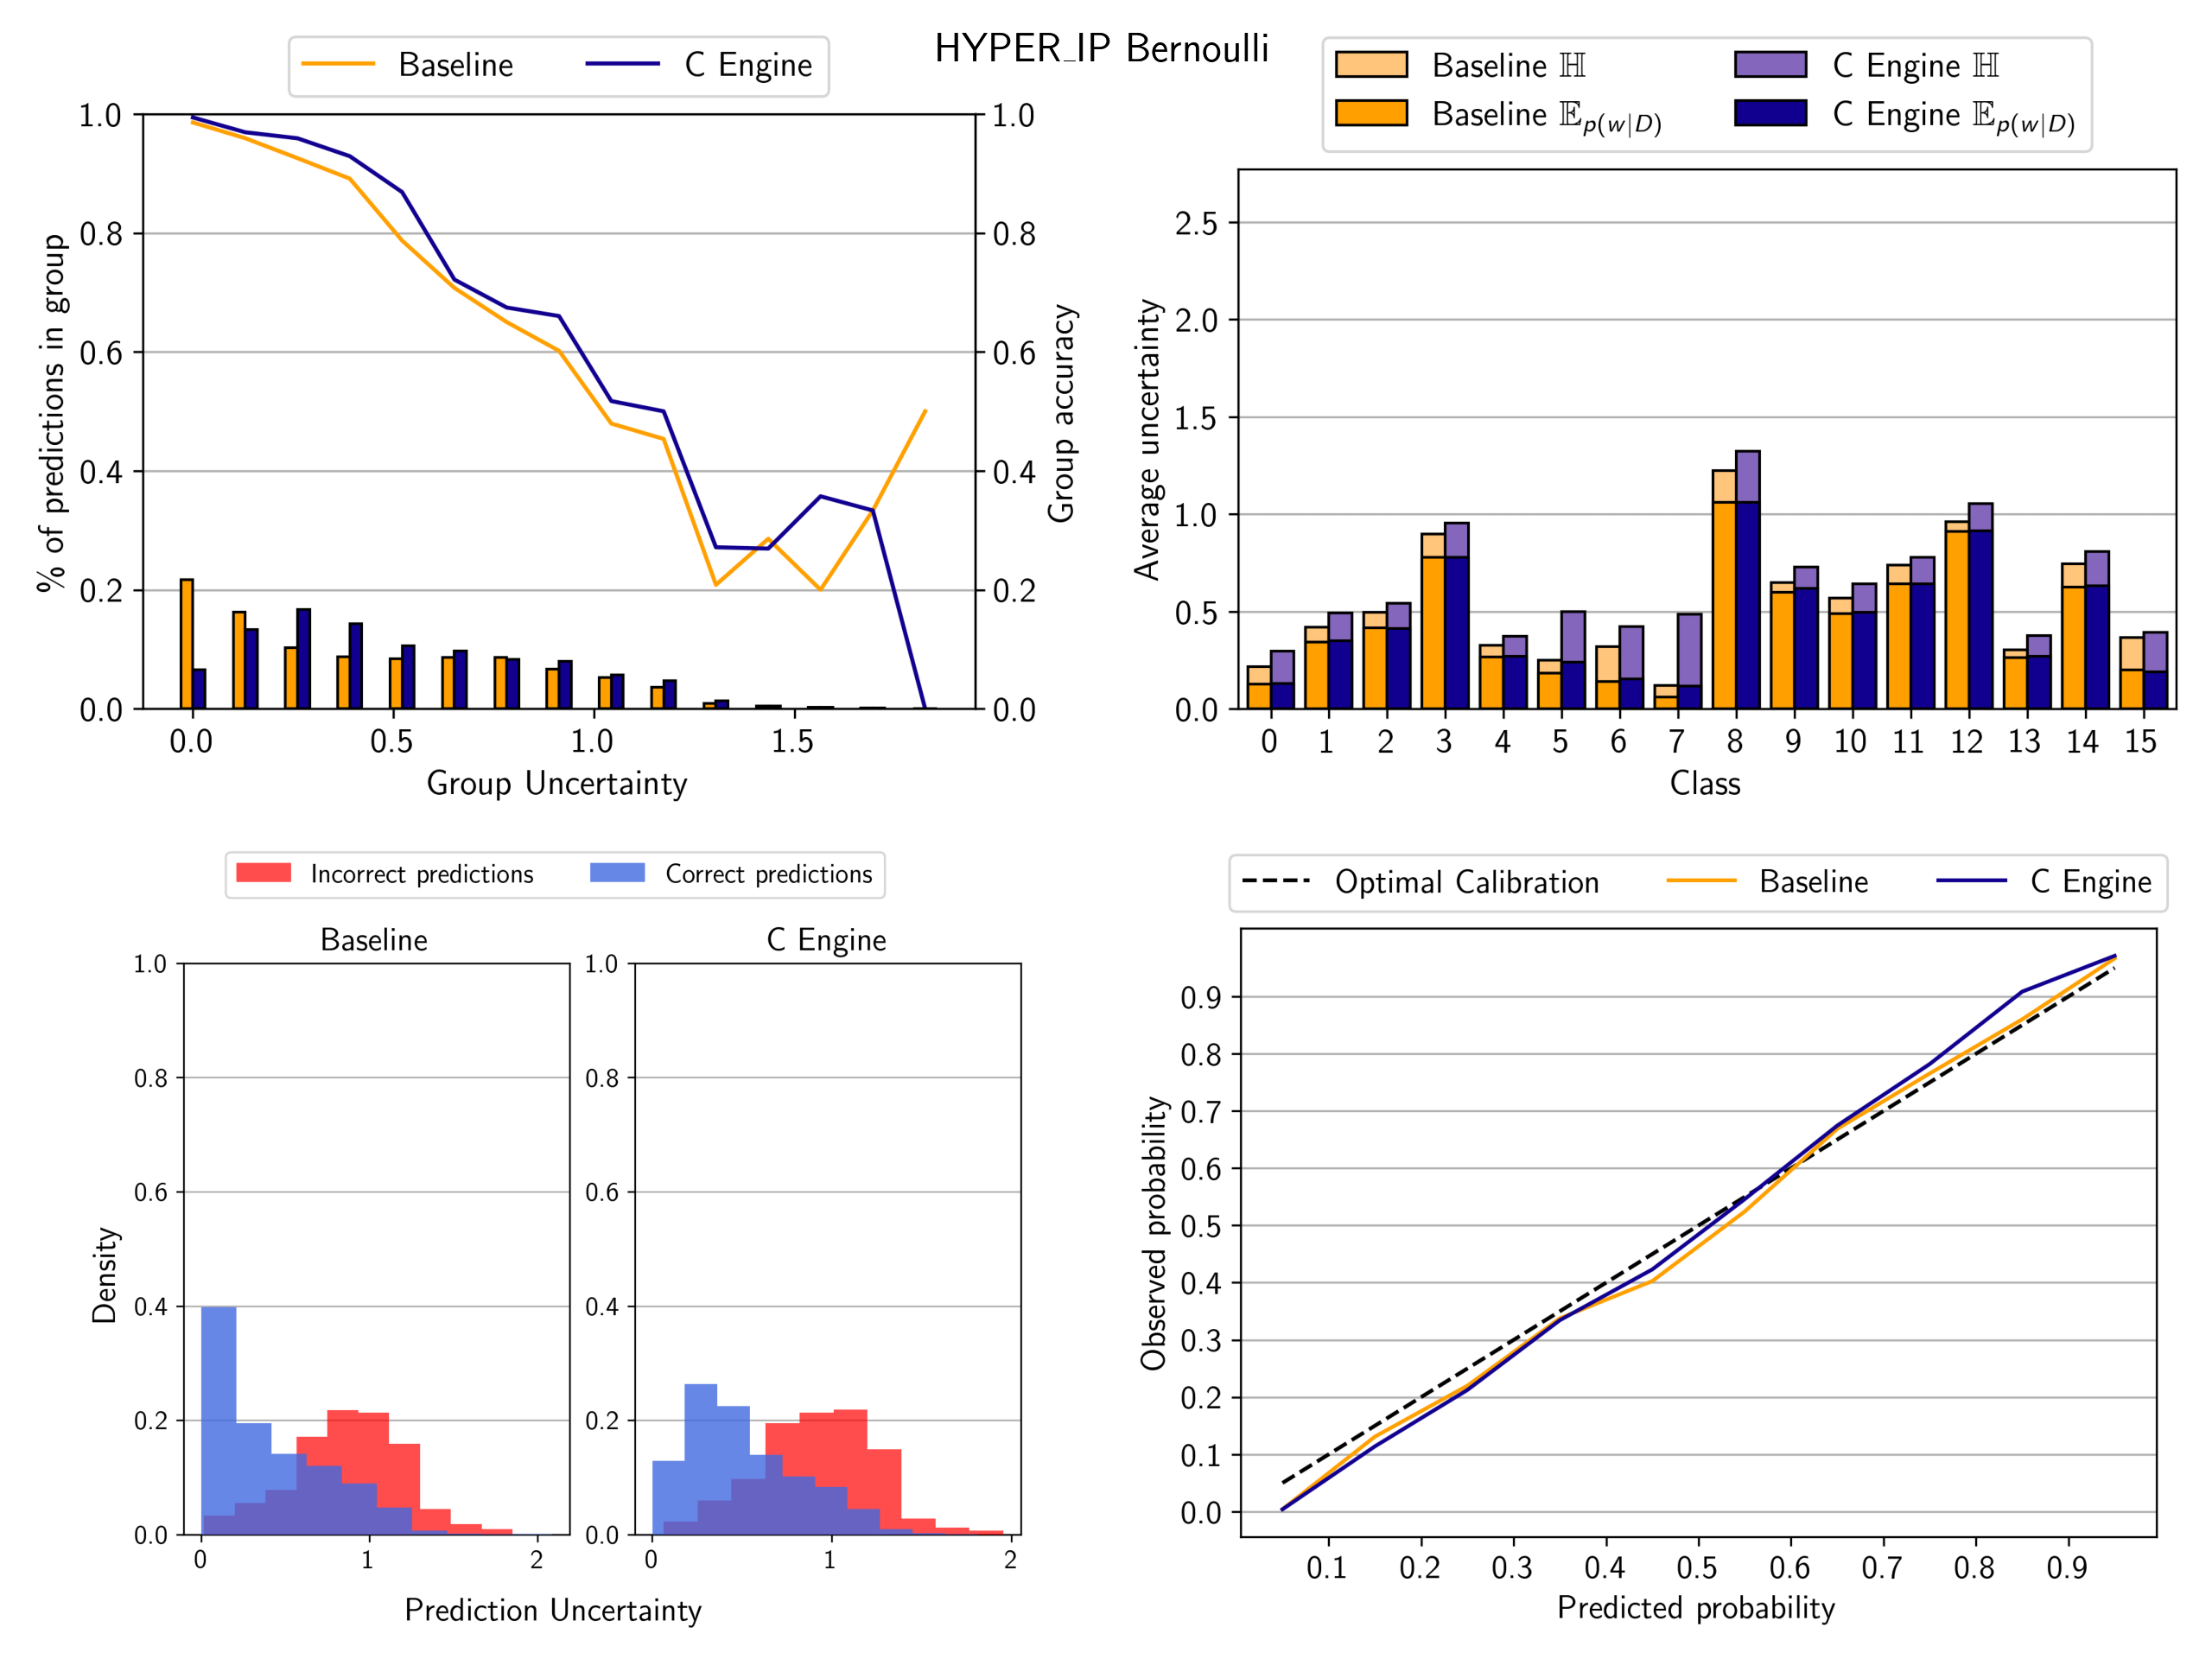
\includegraphics[width=0.9\textwidth]{root/Imagenes/anexo/Bernoulli-HYPER_IP-mosaic.png}
    \caption{Predicciones del conjunto de prueba de píxeles hiperespectrales IP.}
    \label{fig:anx-Bernoulli-HYPER_IP}
\end{figure}


\begin{figure}[ht]
    \centering
    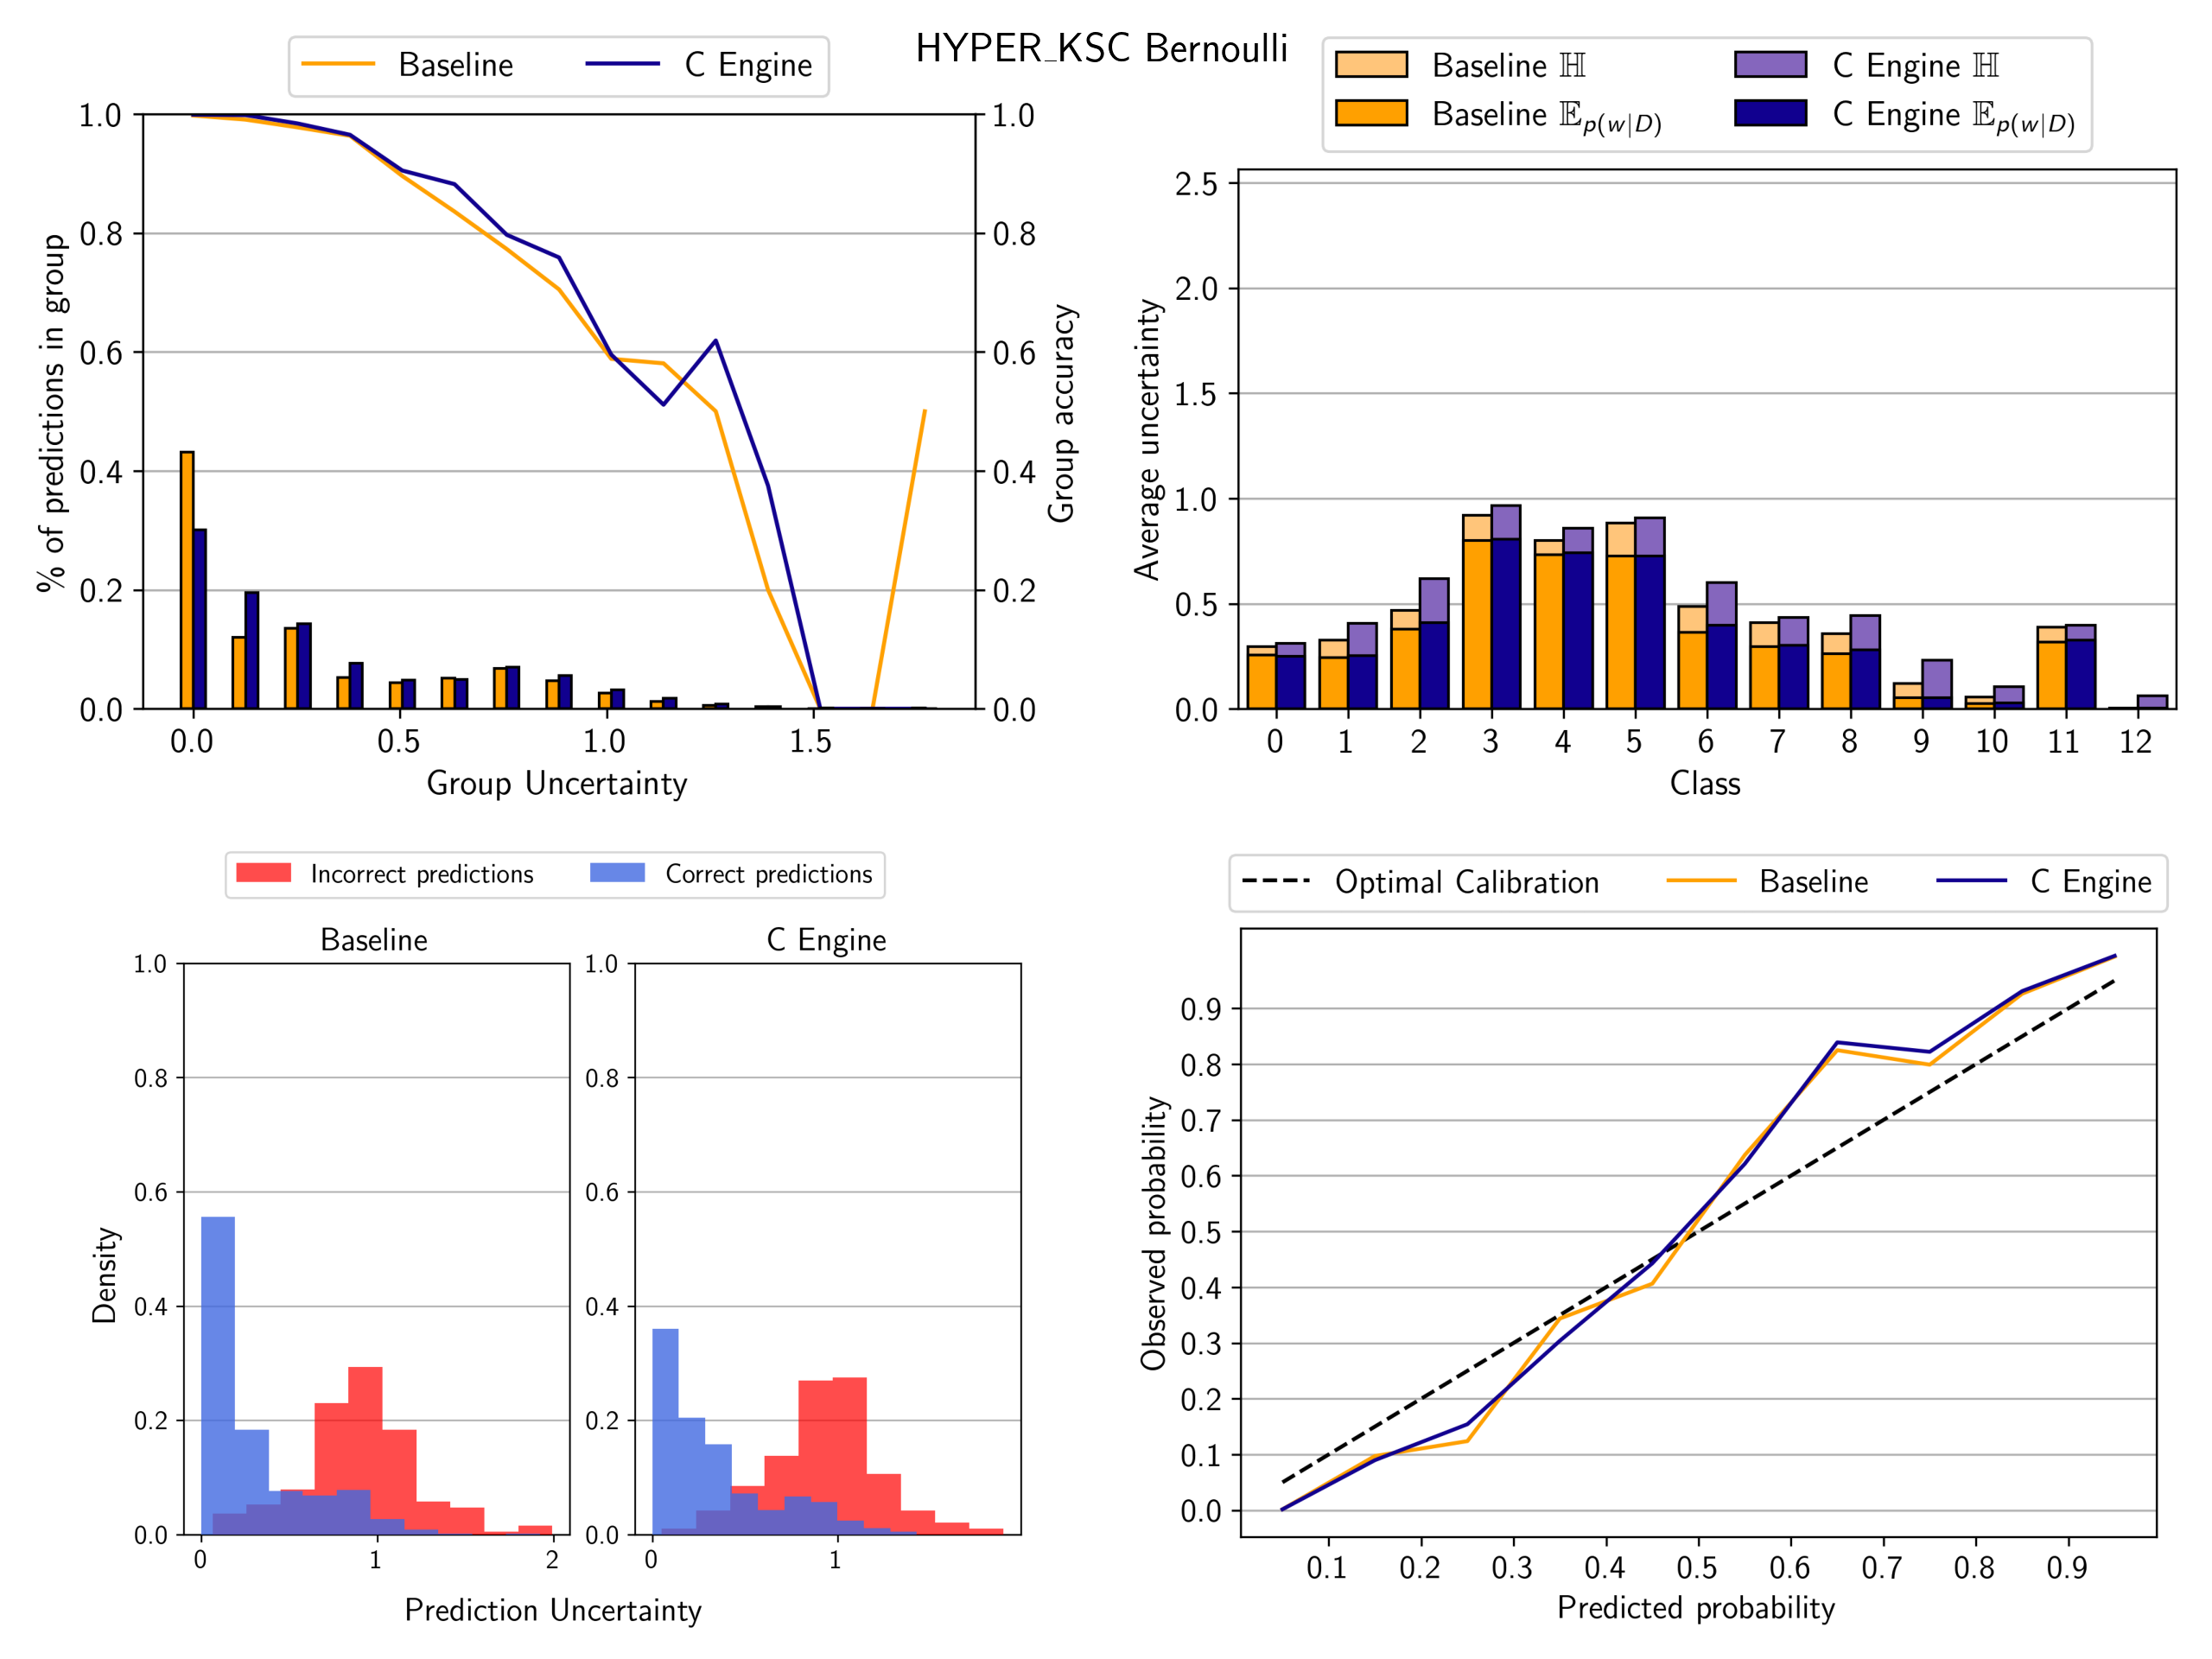
\includegraphics[width=0.9\textwidth]{root/Imagenes/anexo/Bernoulli-HYPER_KSC-mosaic.png}
    \caption{Predicciones del conjunto de prueba de píxeles hiperespectrales KSC.}
    \label{fig:anx-Bernoulli-HYPER_KSC}
\end{figure}


\begin{figure}[ht]
    \centering
    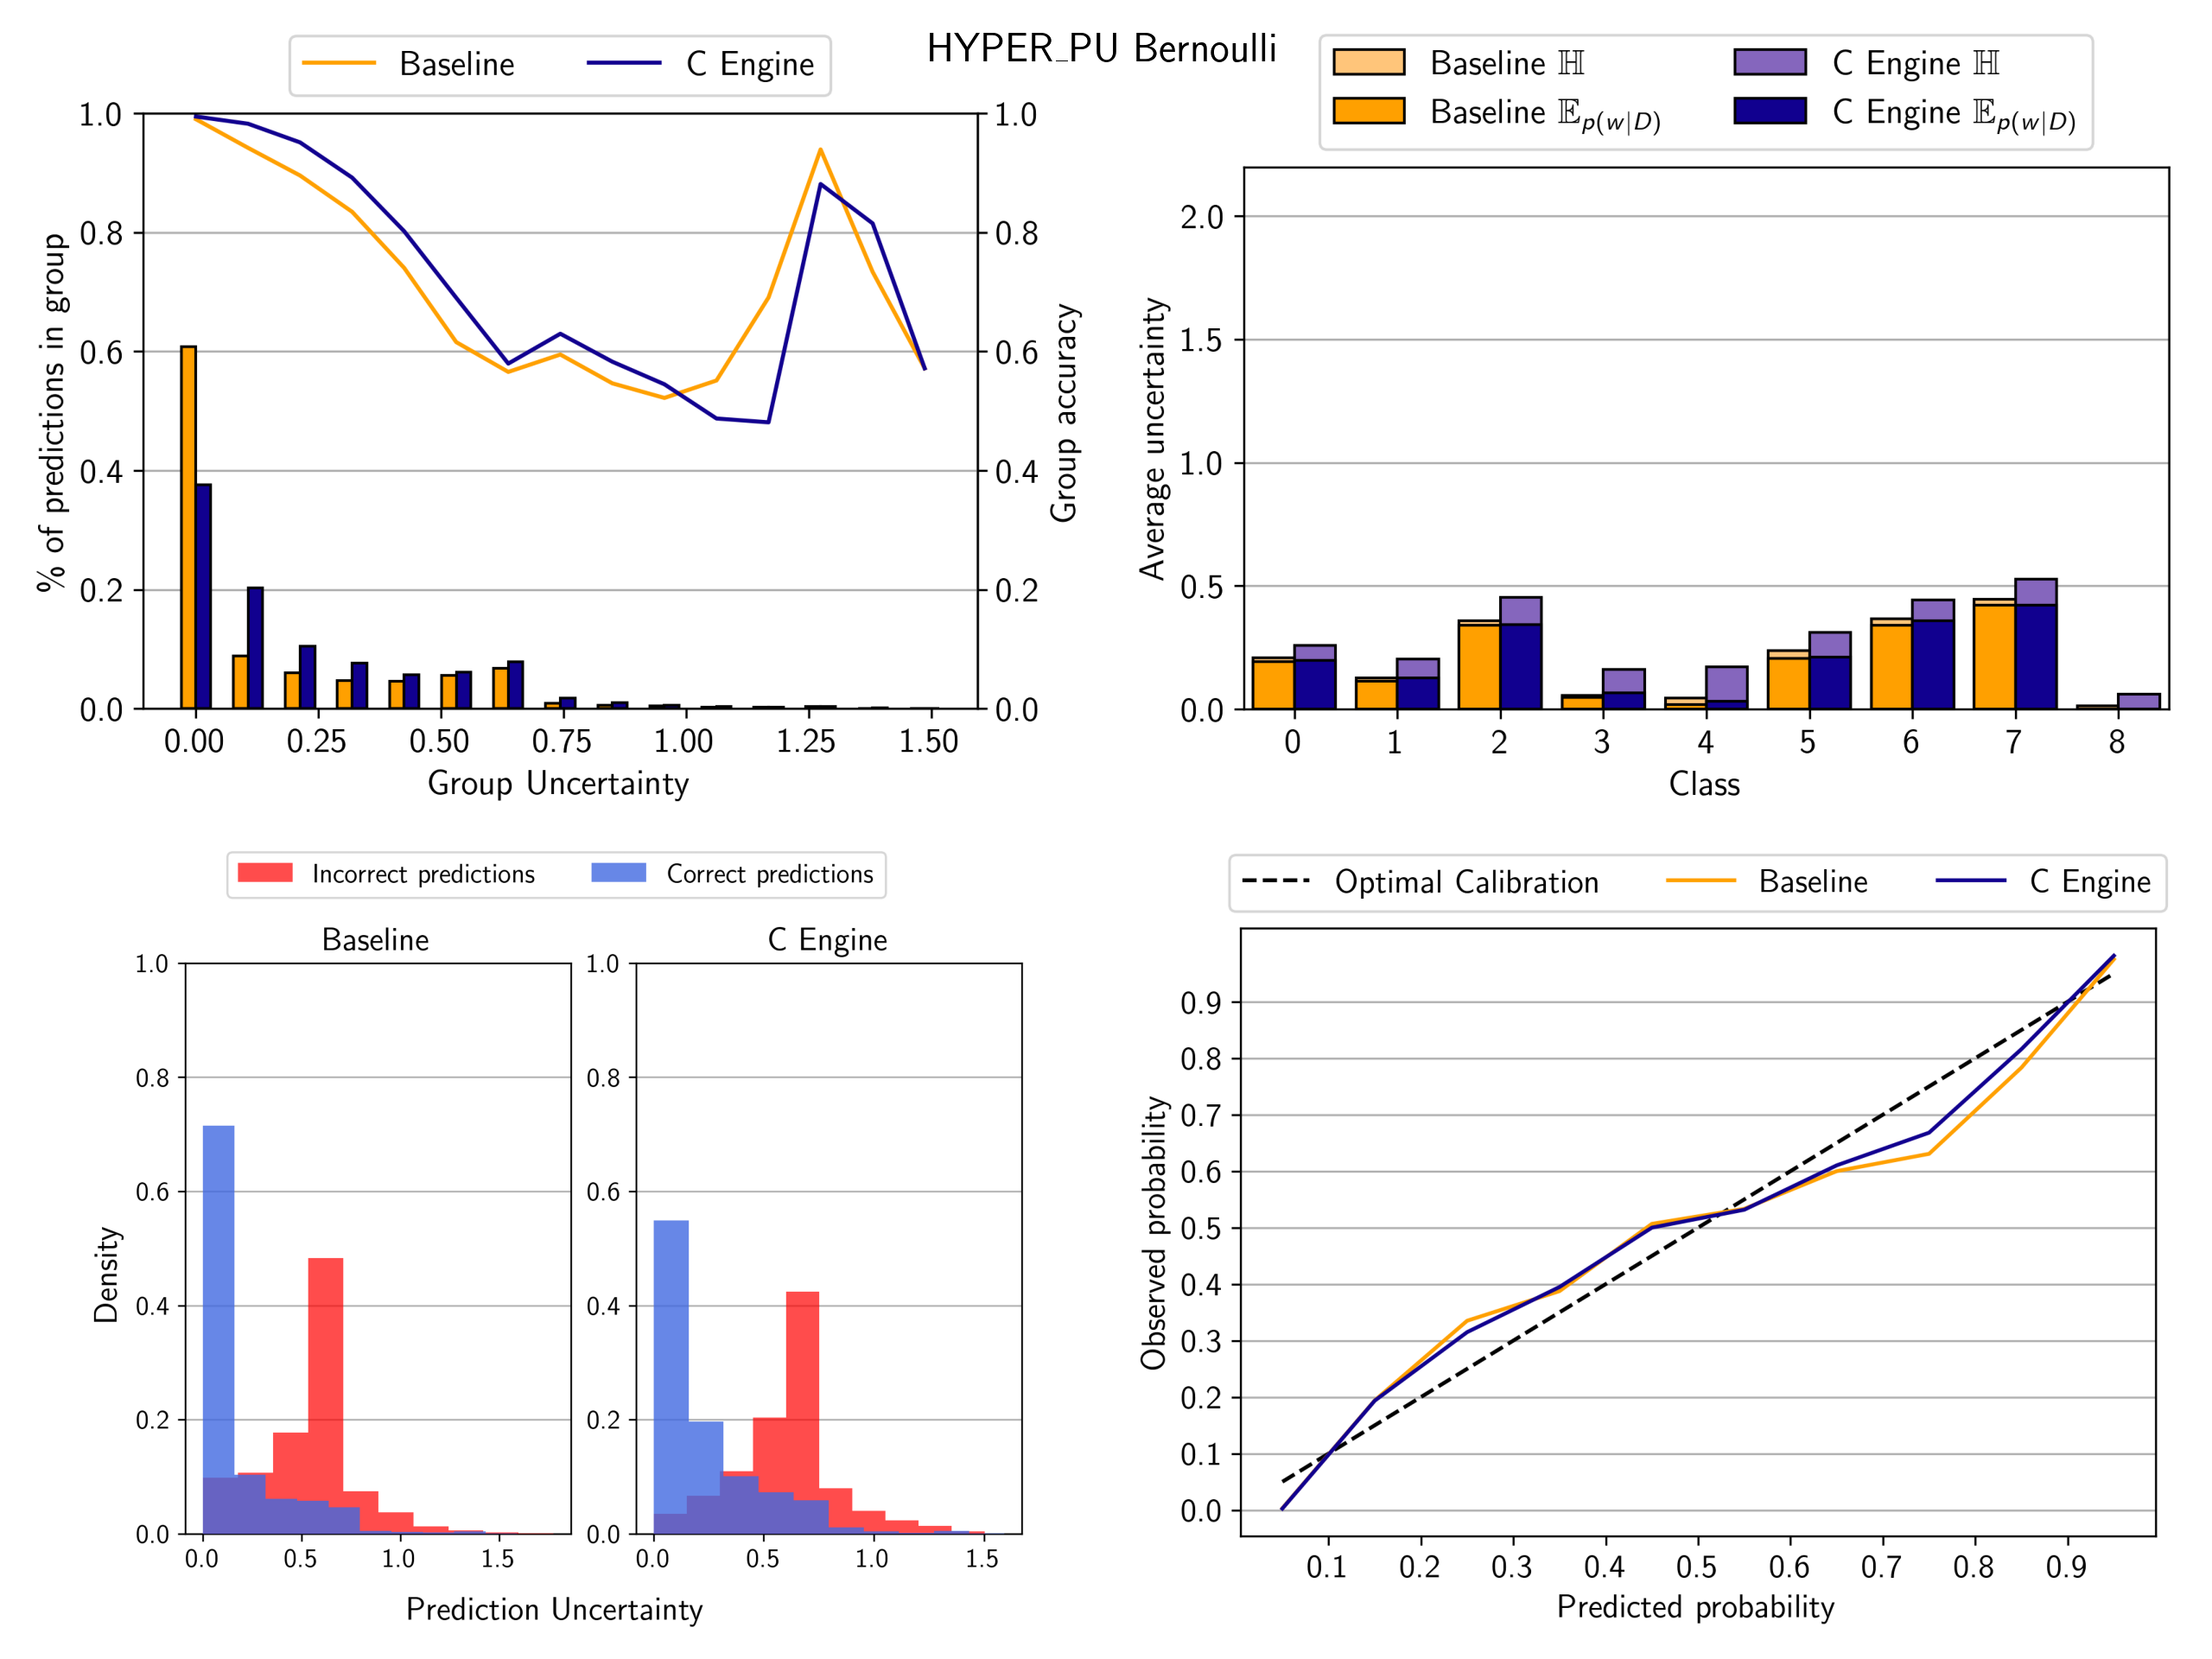
\includegraphics[width=0.9\textwidth]{root/Imagenes/anexo/Bernoulli-HYPER_PU-mosaic.png}
    \caption{Predicciones del conjunto de prueba de píxeles hiperespectrales PU.}
    \label{fig:anx-Bernoulli-HYPER_PU}
\end{figure}


\begin{figure}[ht]
    \centering
    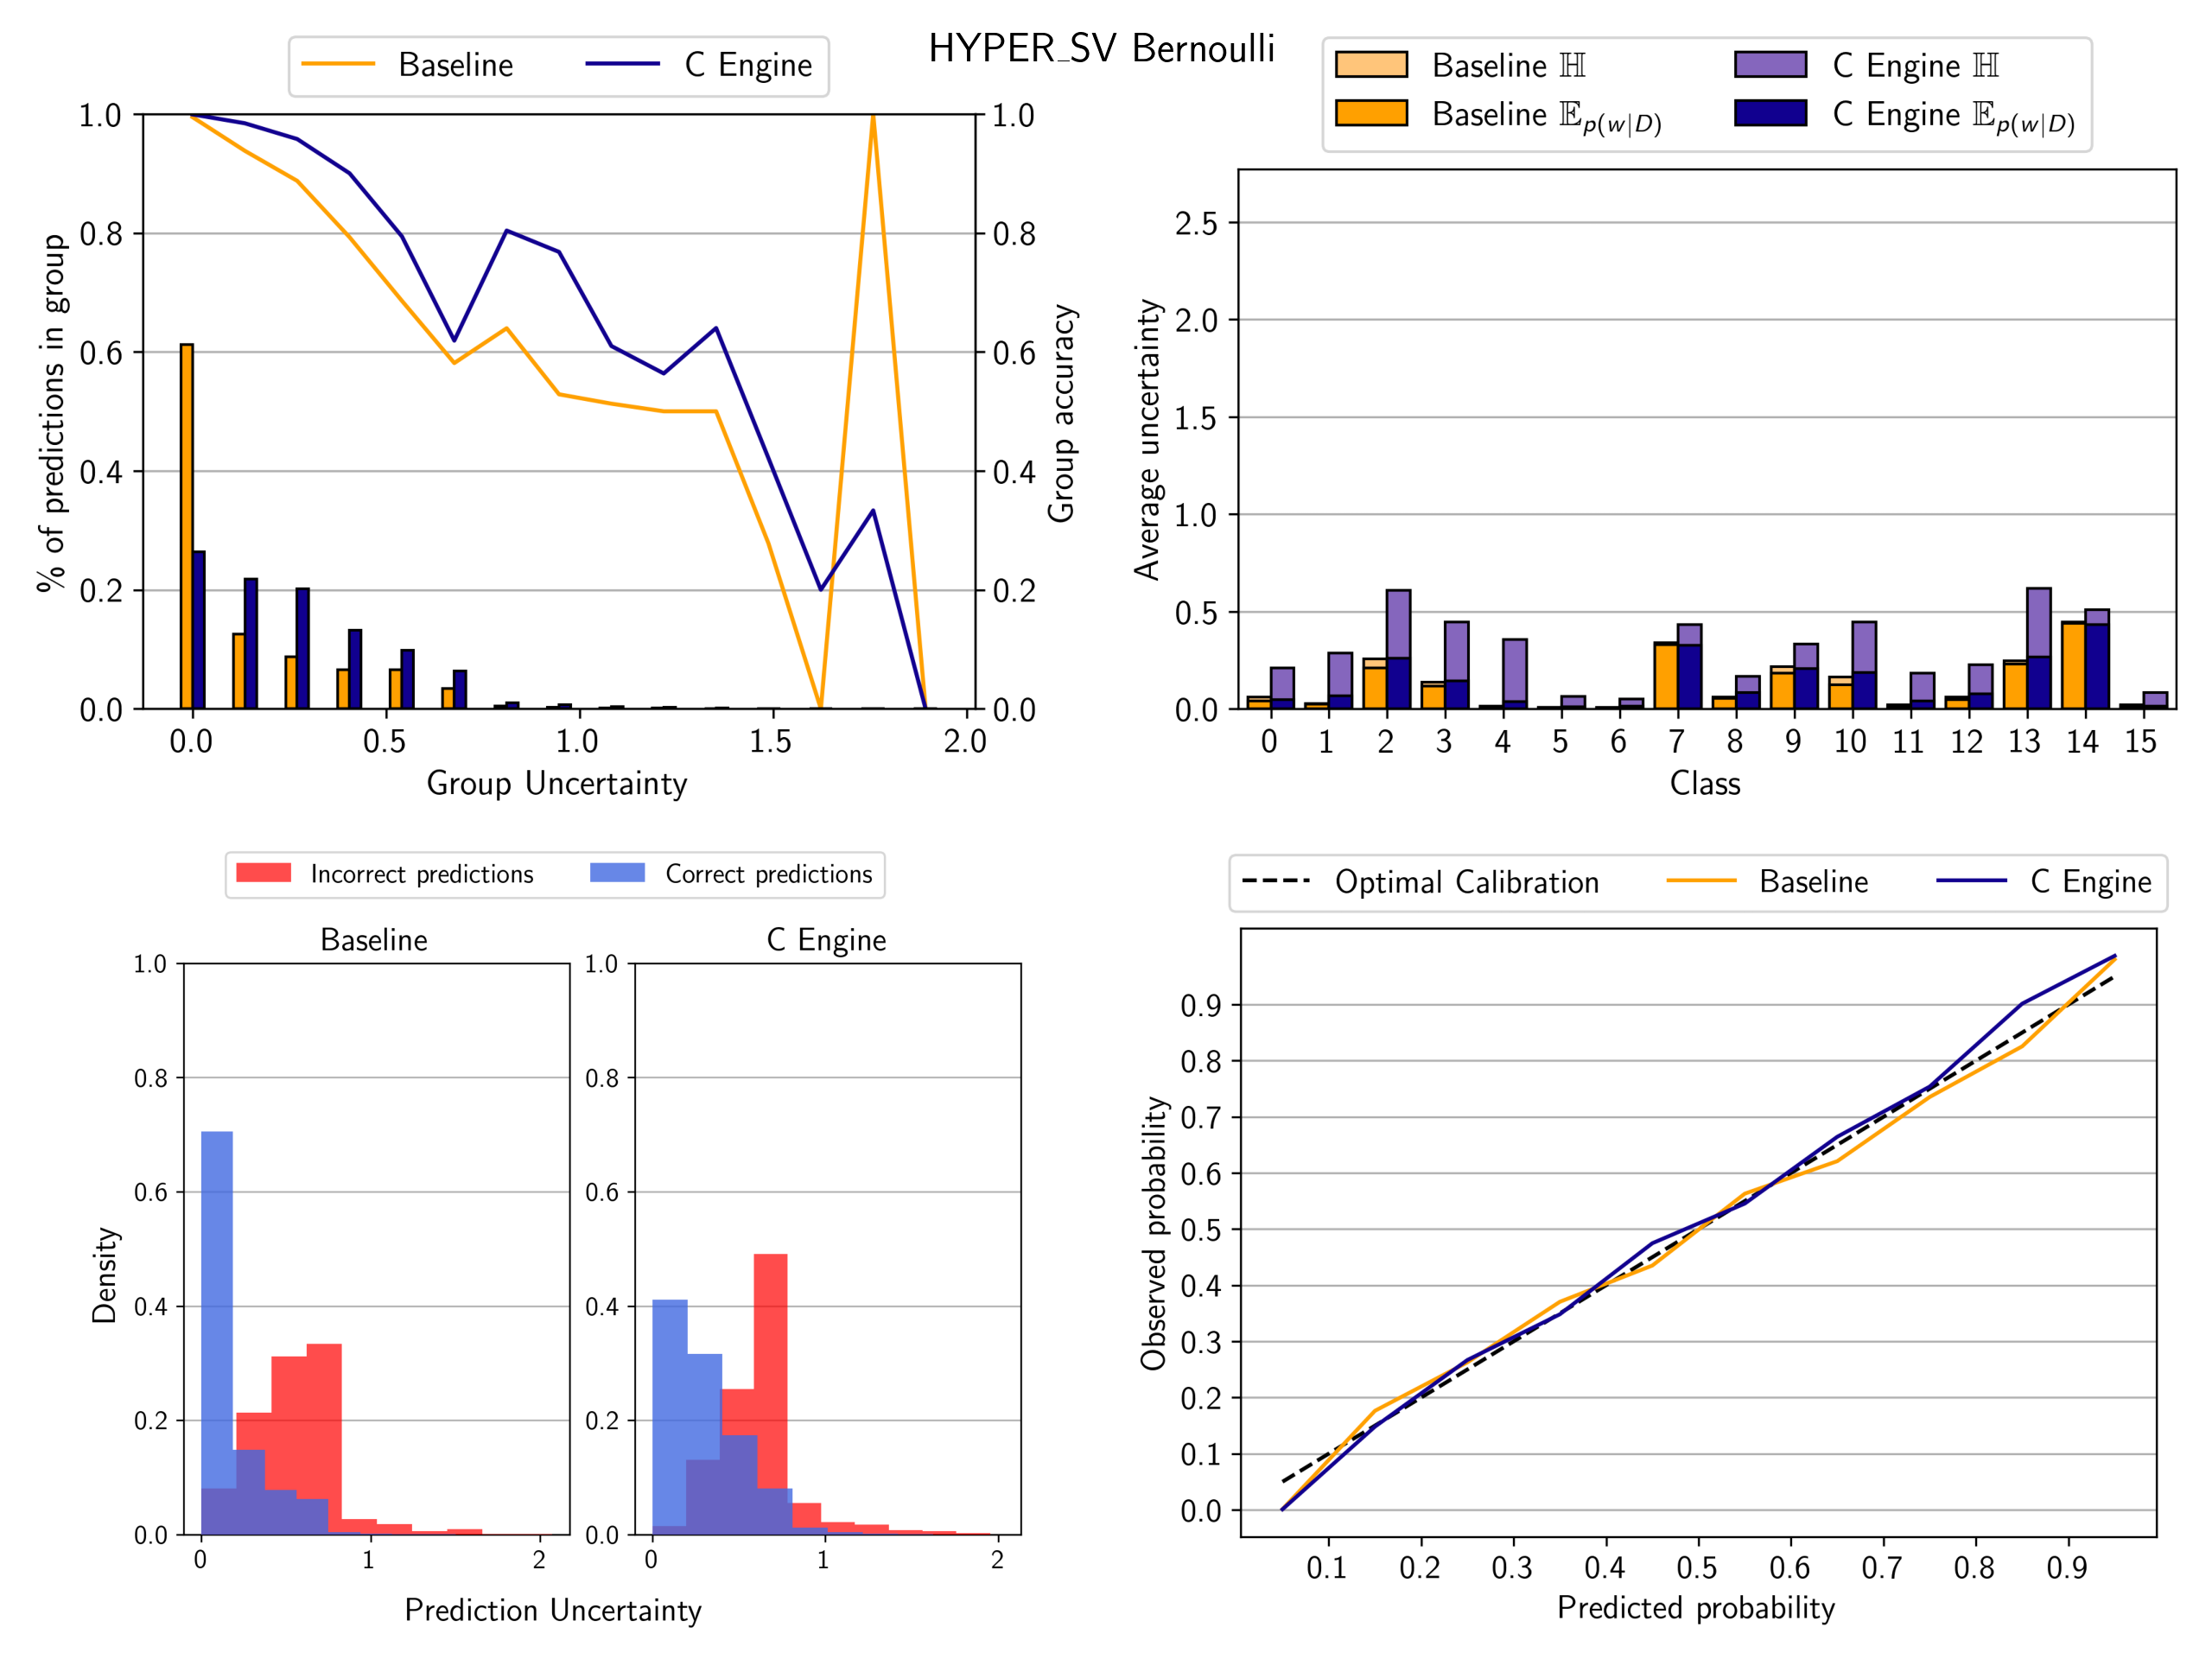
\includegraphics[width=0.9\textwidth]{root/Imagenes/anexo/Bernoulli-HYPER_SV-mosaic.png}
    \caption{Predicciones del conjunto de prueba de píxeles hiperespectrales SV.}
    \label{fig:anx-Bernoulli-HYPER_SV}
\end{figure}


\begin{figure}[ht]
    \centering
    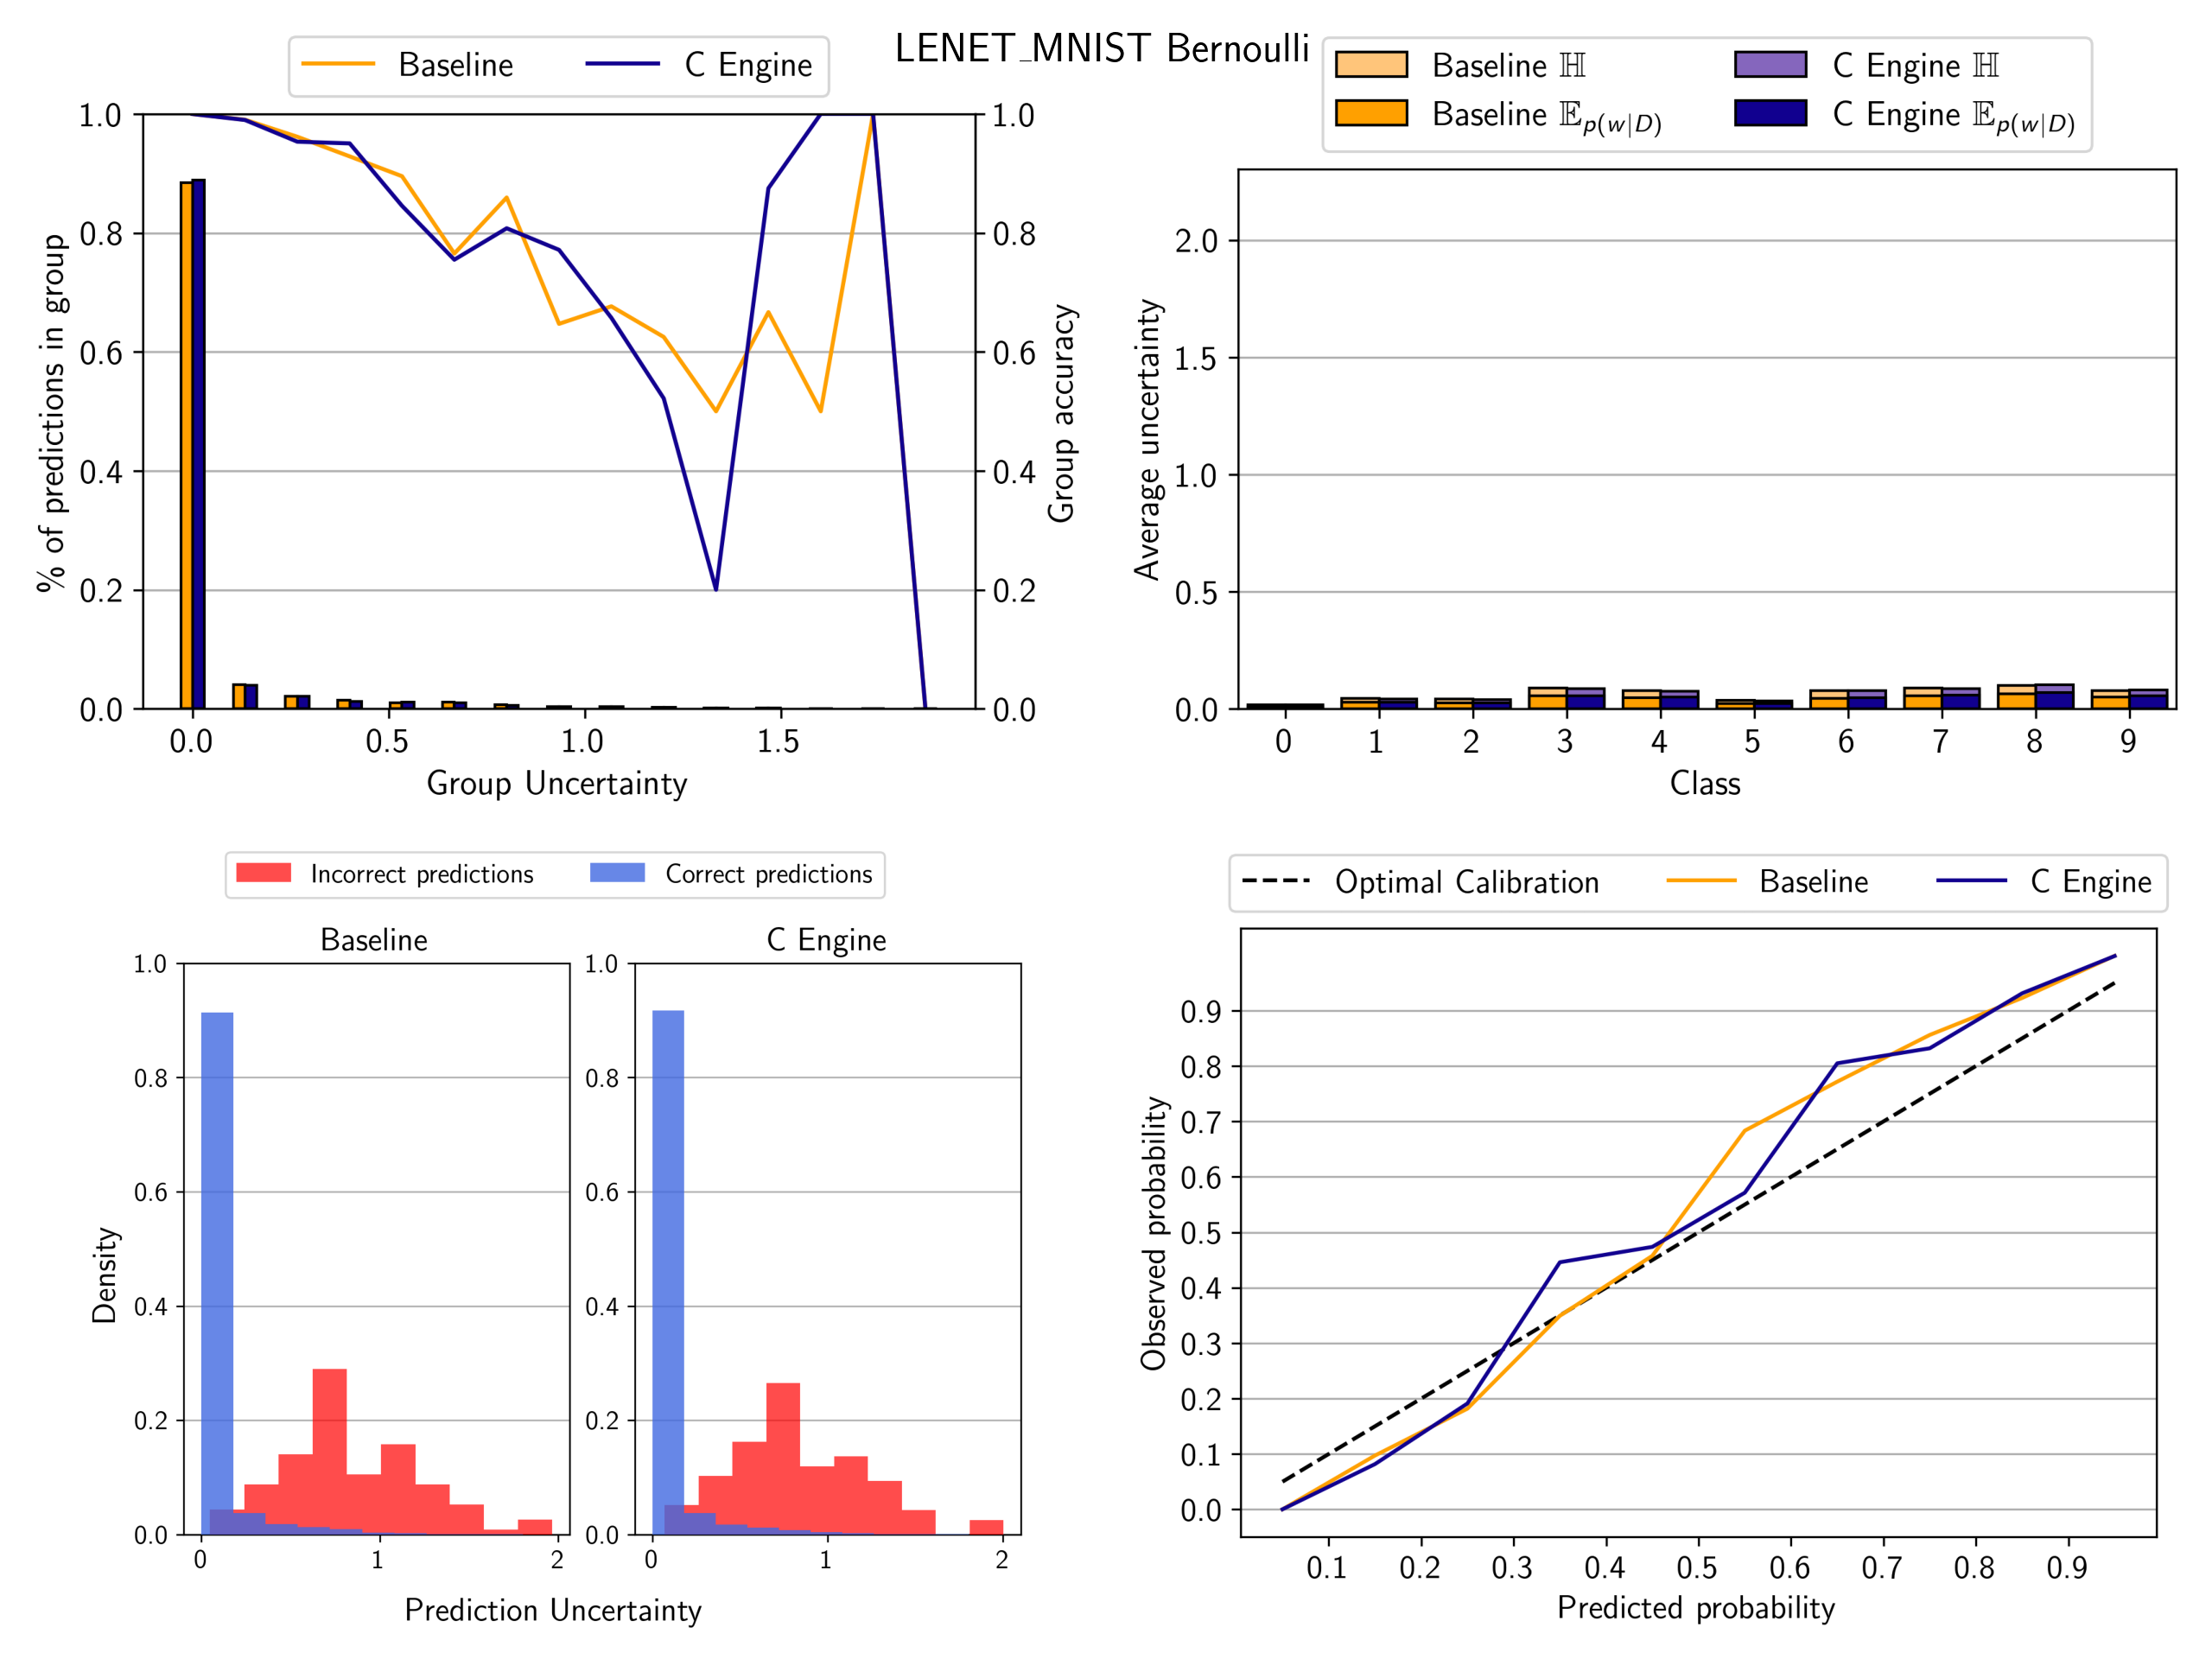
\includegraphics[width=0.9\textwidth]{root/Imagenes/anexo/Bernoulli-LENET_MNIST-mosaic.png}
    \caption{Predicciones del modelo LENET con el conjunto de datos MNIST.}
    \label{fig:anx-Bernoulli-LENET_MNIST}
\end{figure}


\begin{figure}[ht]
    \centering
    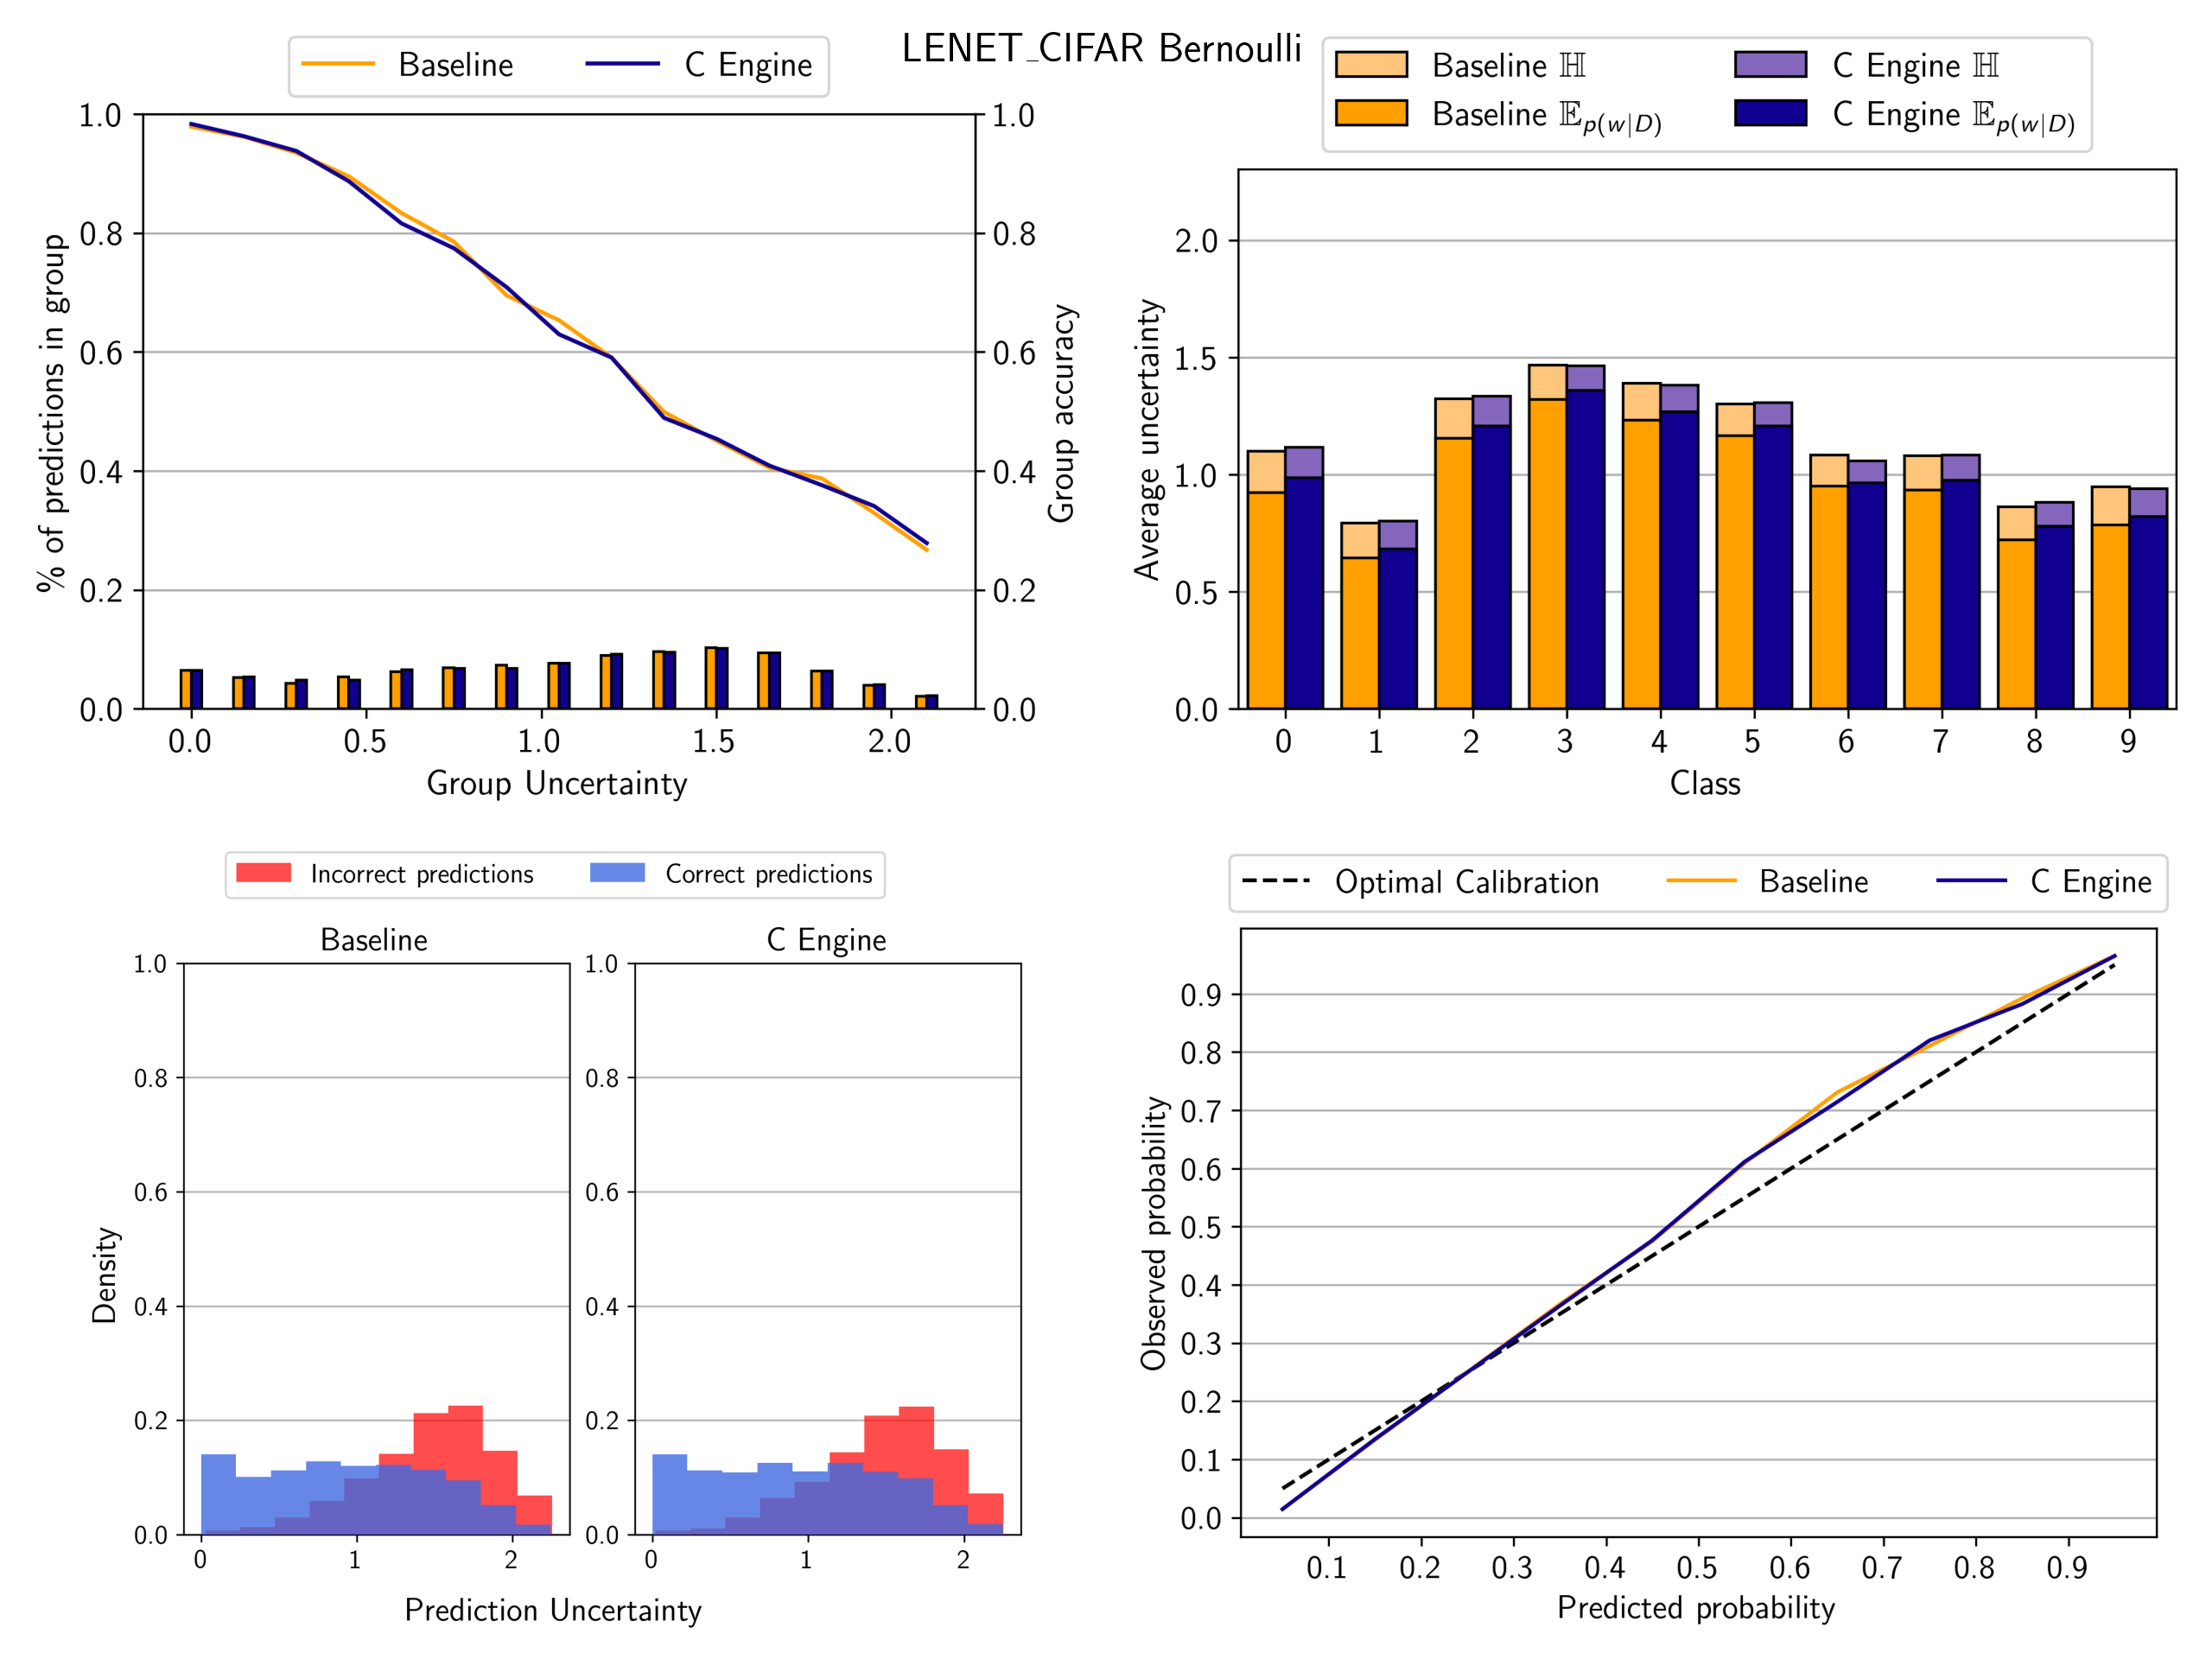
\includegraphics[width=0.9\textwidth]{root/Imagenes/anexo/Bernoulli-LENET_CIFAR-mosaic.png}
    \caption{Predicciones del modelo LENET con el conjunto de datos CIFAR-10.}
    \label{fig:anx-Bernoulli-LENET_CIFAR}
\end{figure}


\begin{figure}[ht]
    \centering
    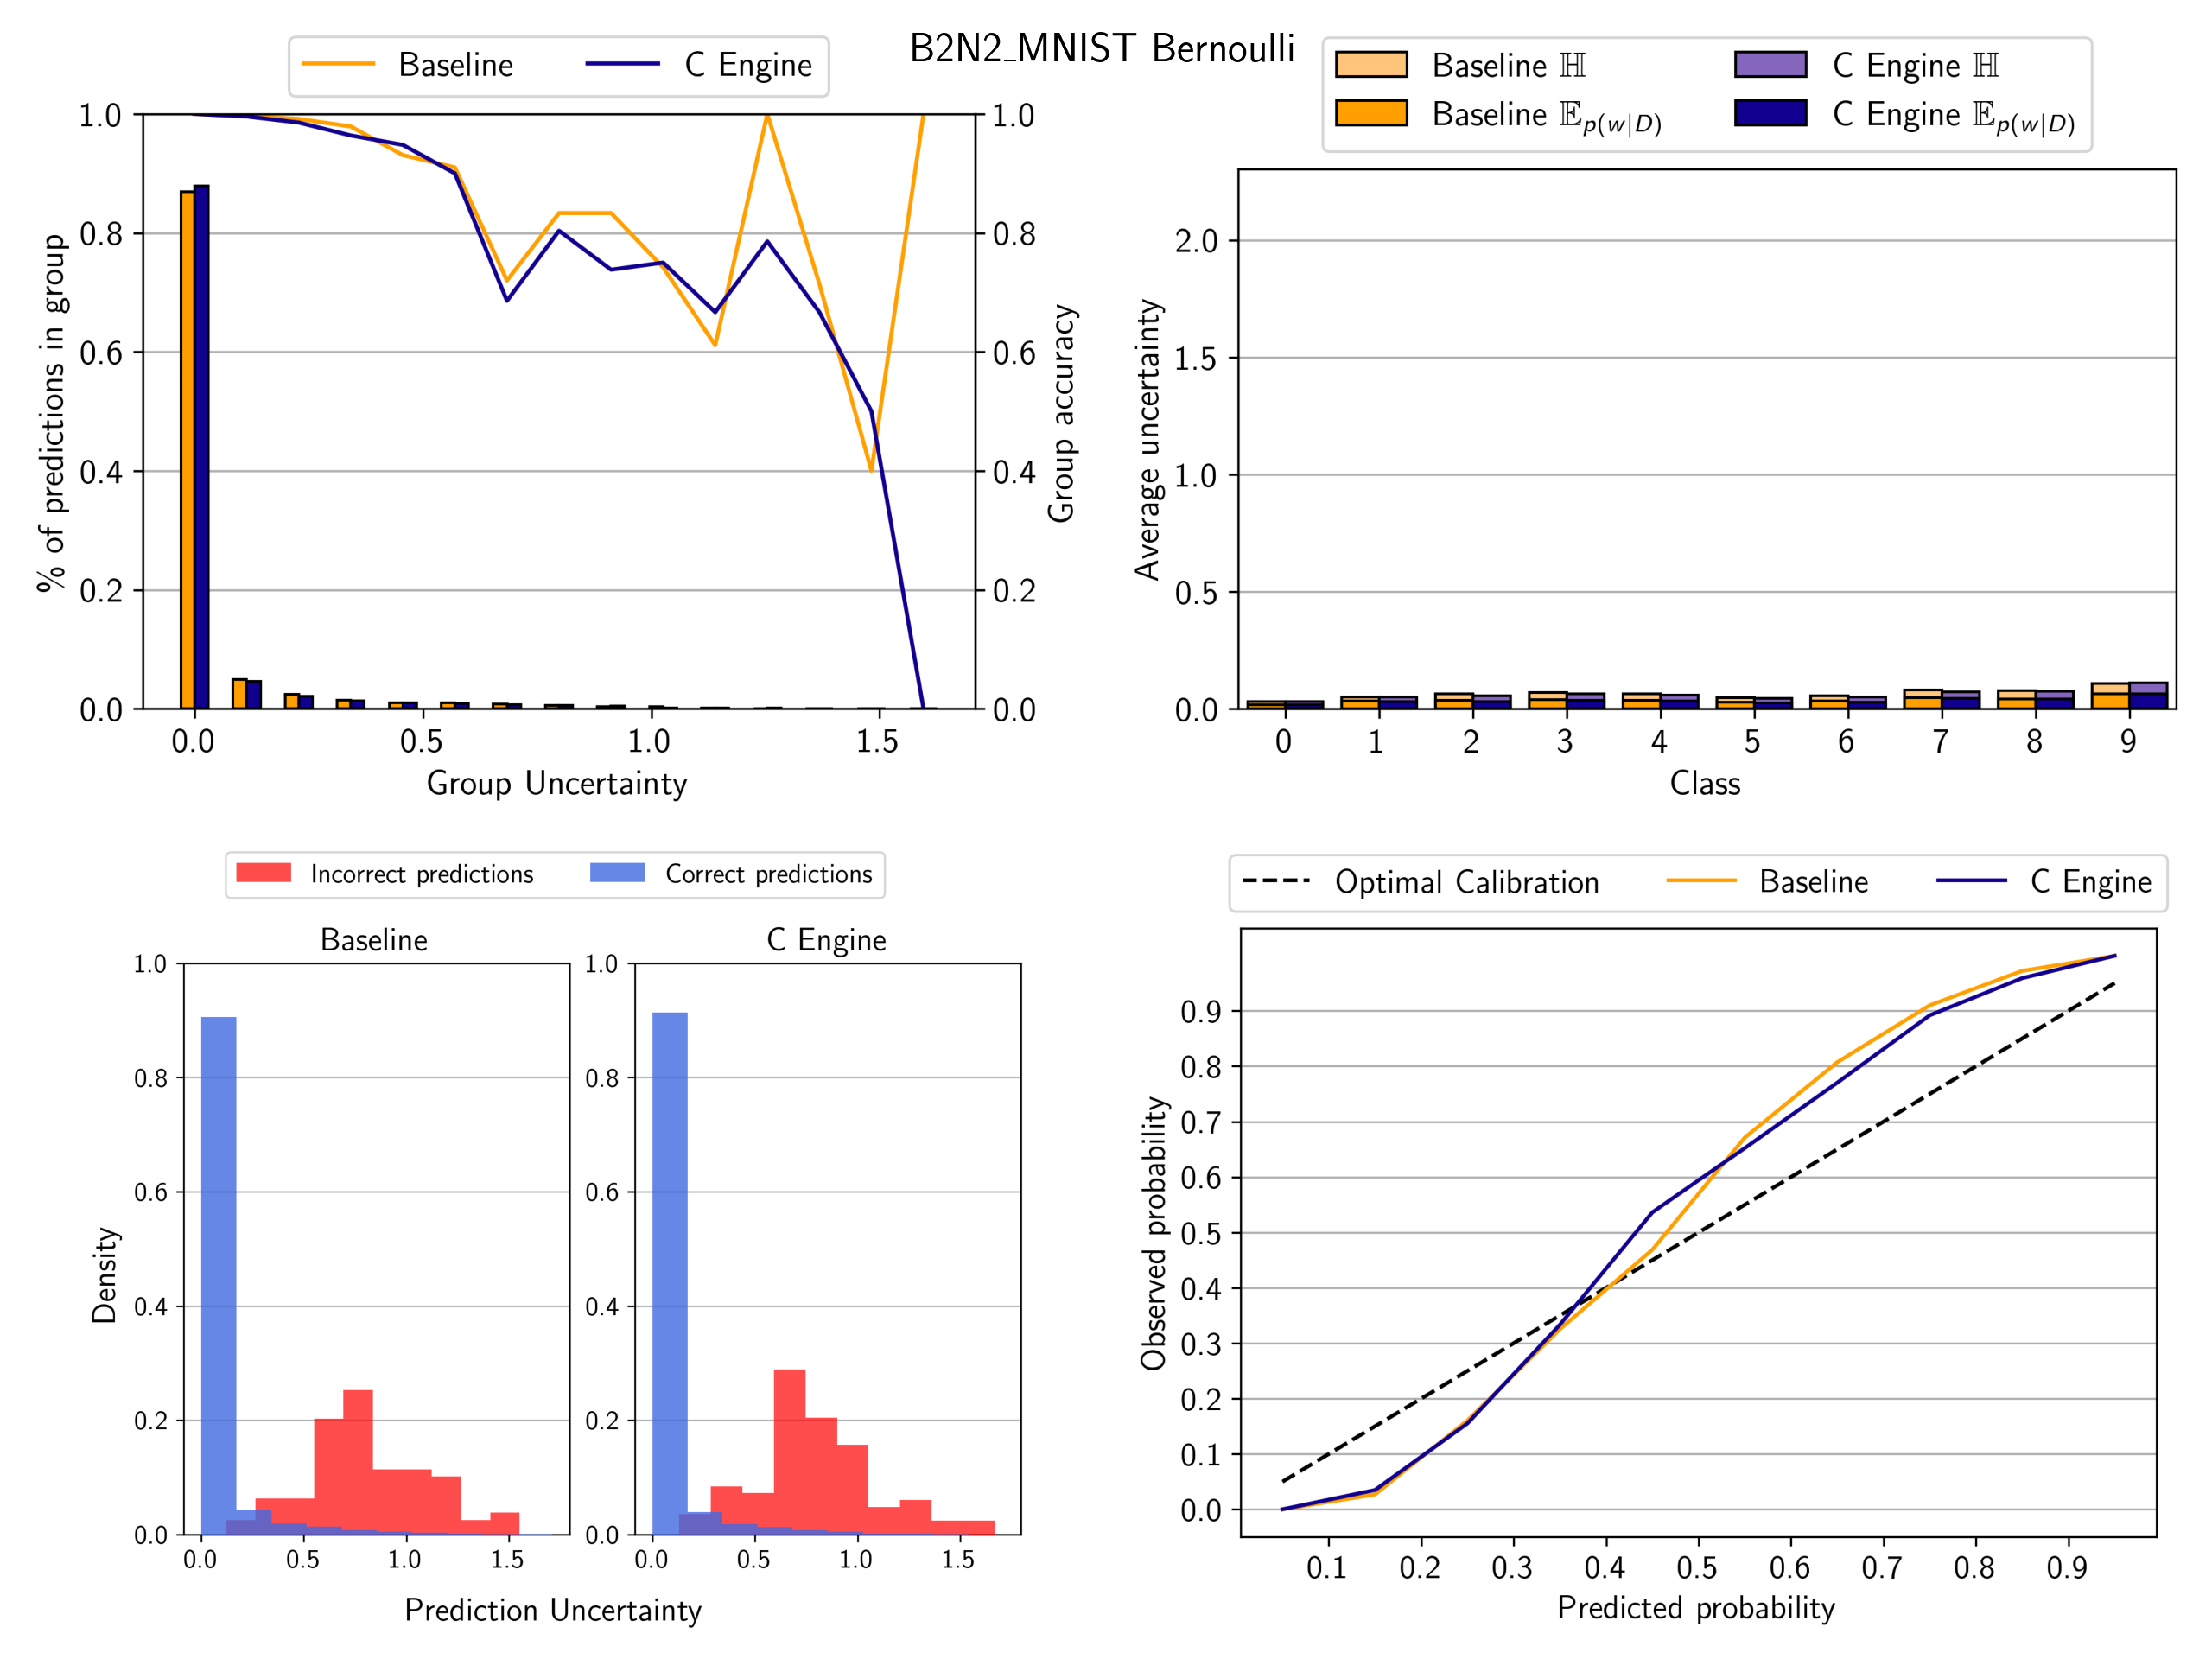
\includegraphics[width=0.9\textwidth]{root/Imagenes/anexo/Bernoulli-B2N2_MNIST-mosaic.png}
    \caption{Predicciones del modelo B2N2 con el conjunto de datos MNIST.}
    \label{fig:anx-Bernoulli-B2N2_MNIST}
\end{figure}


\begin{figure}[ht]
    \centering
    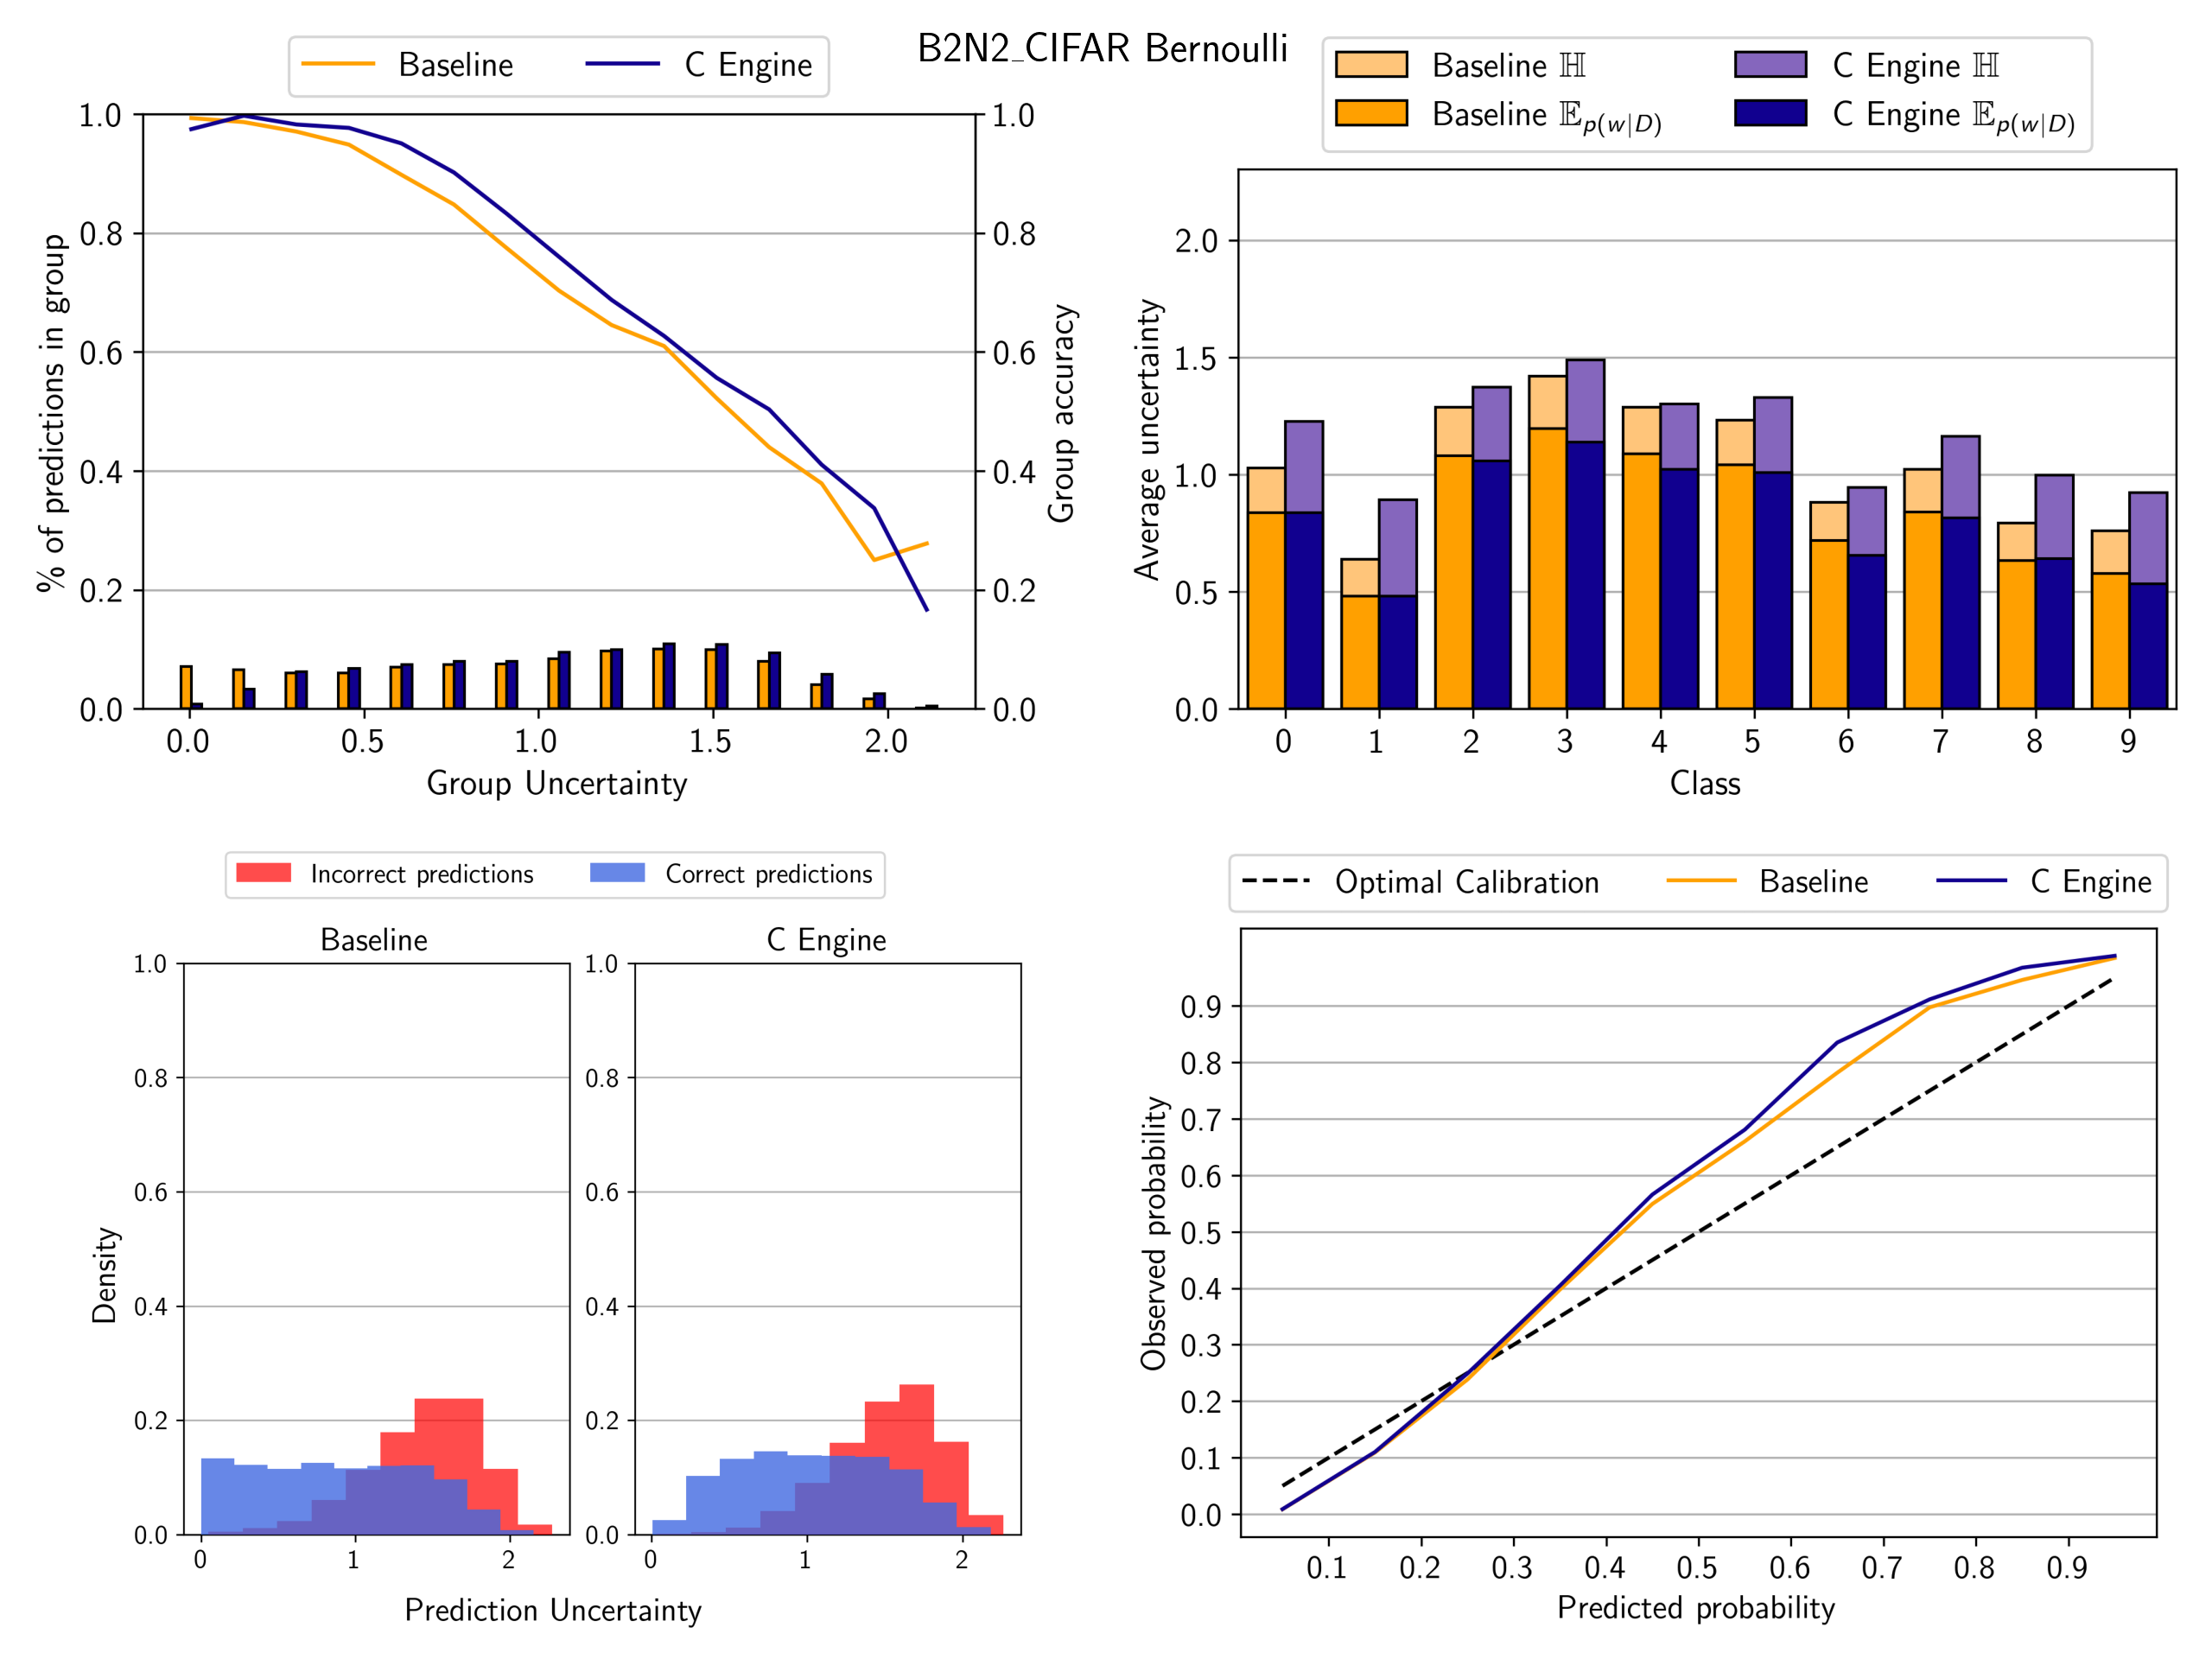
\includegraphics[width=0.9\textwidth]{root/Imagenes/anexo/Bernoulli-B2N2_CIFAR-mosaic.png}
    \caption{Predicciones del modelo B2N2 con el conjunto de datos CIFAR-10.}
    \label{fig:anx-Bernoulli-B2N2_CIFAR}
\end{figure}


\chapter{Resultados de incertidumbre optimización Uniforme} \label{anx:uniforme}

\begin{figure}[ht]
    \centering
    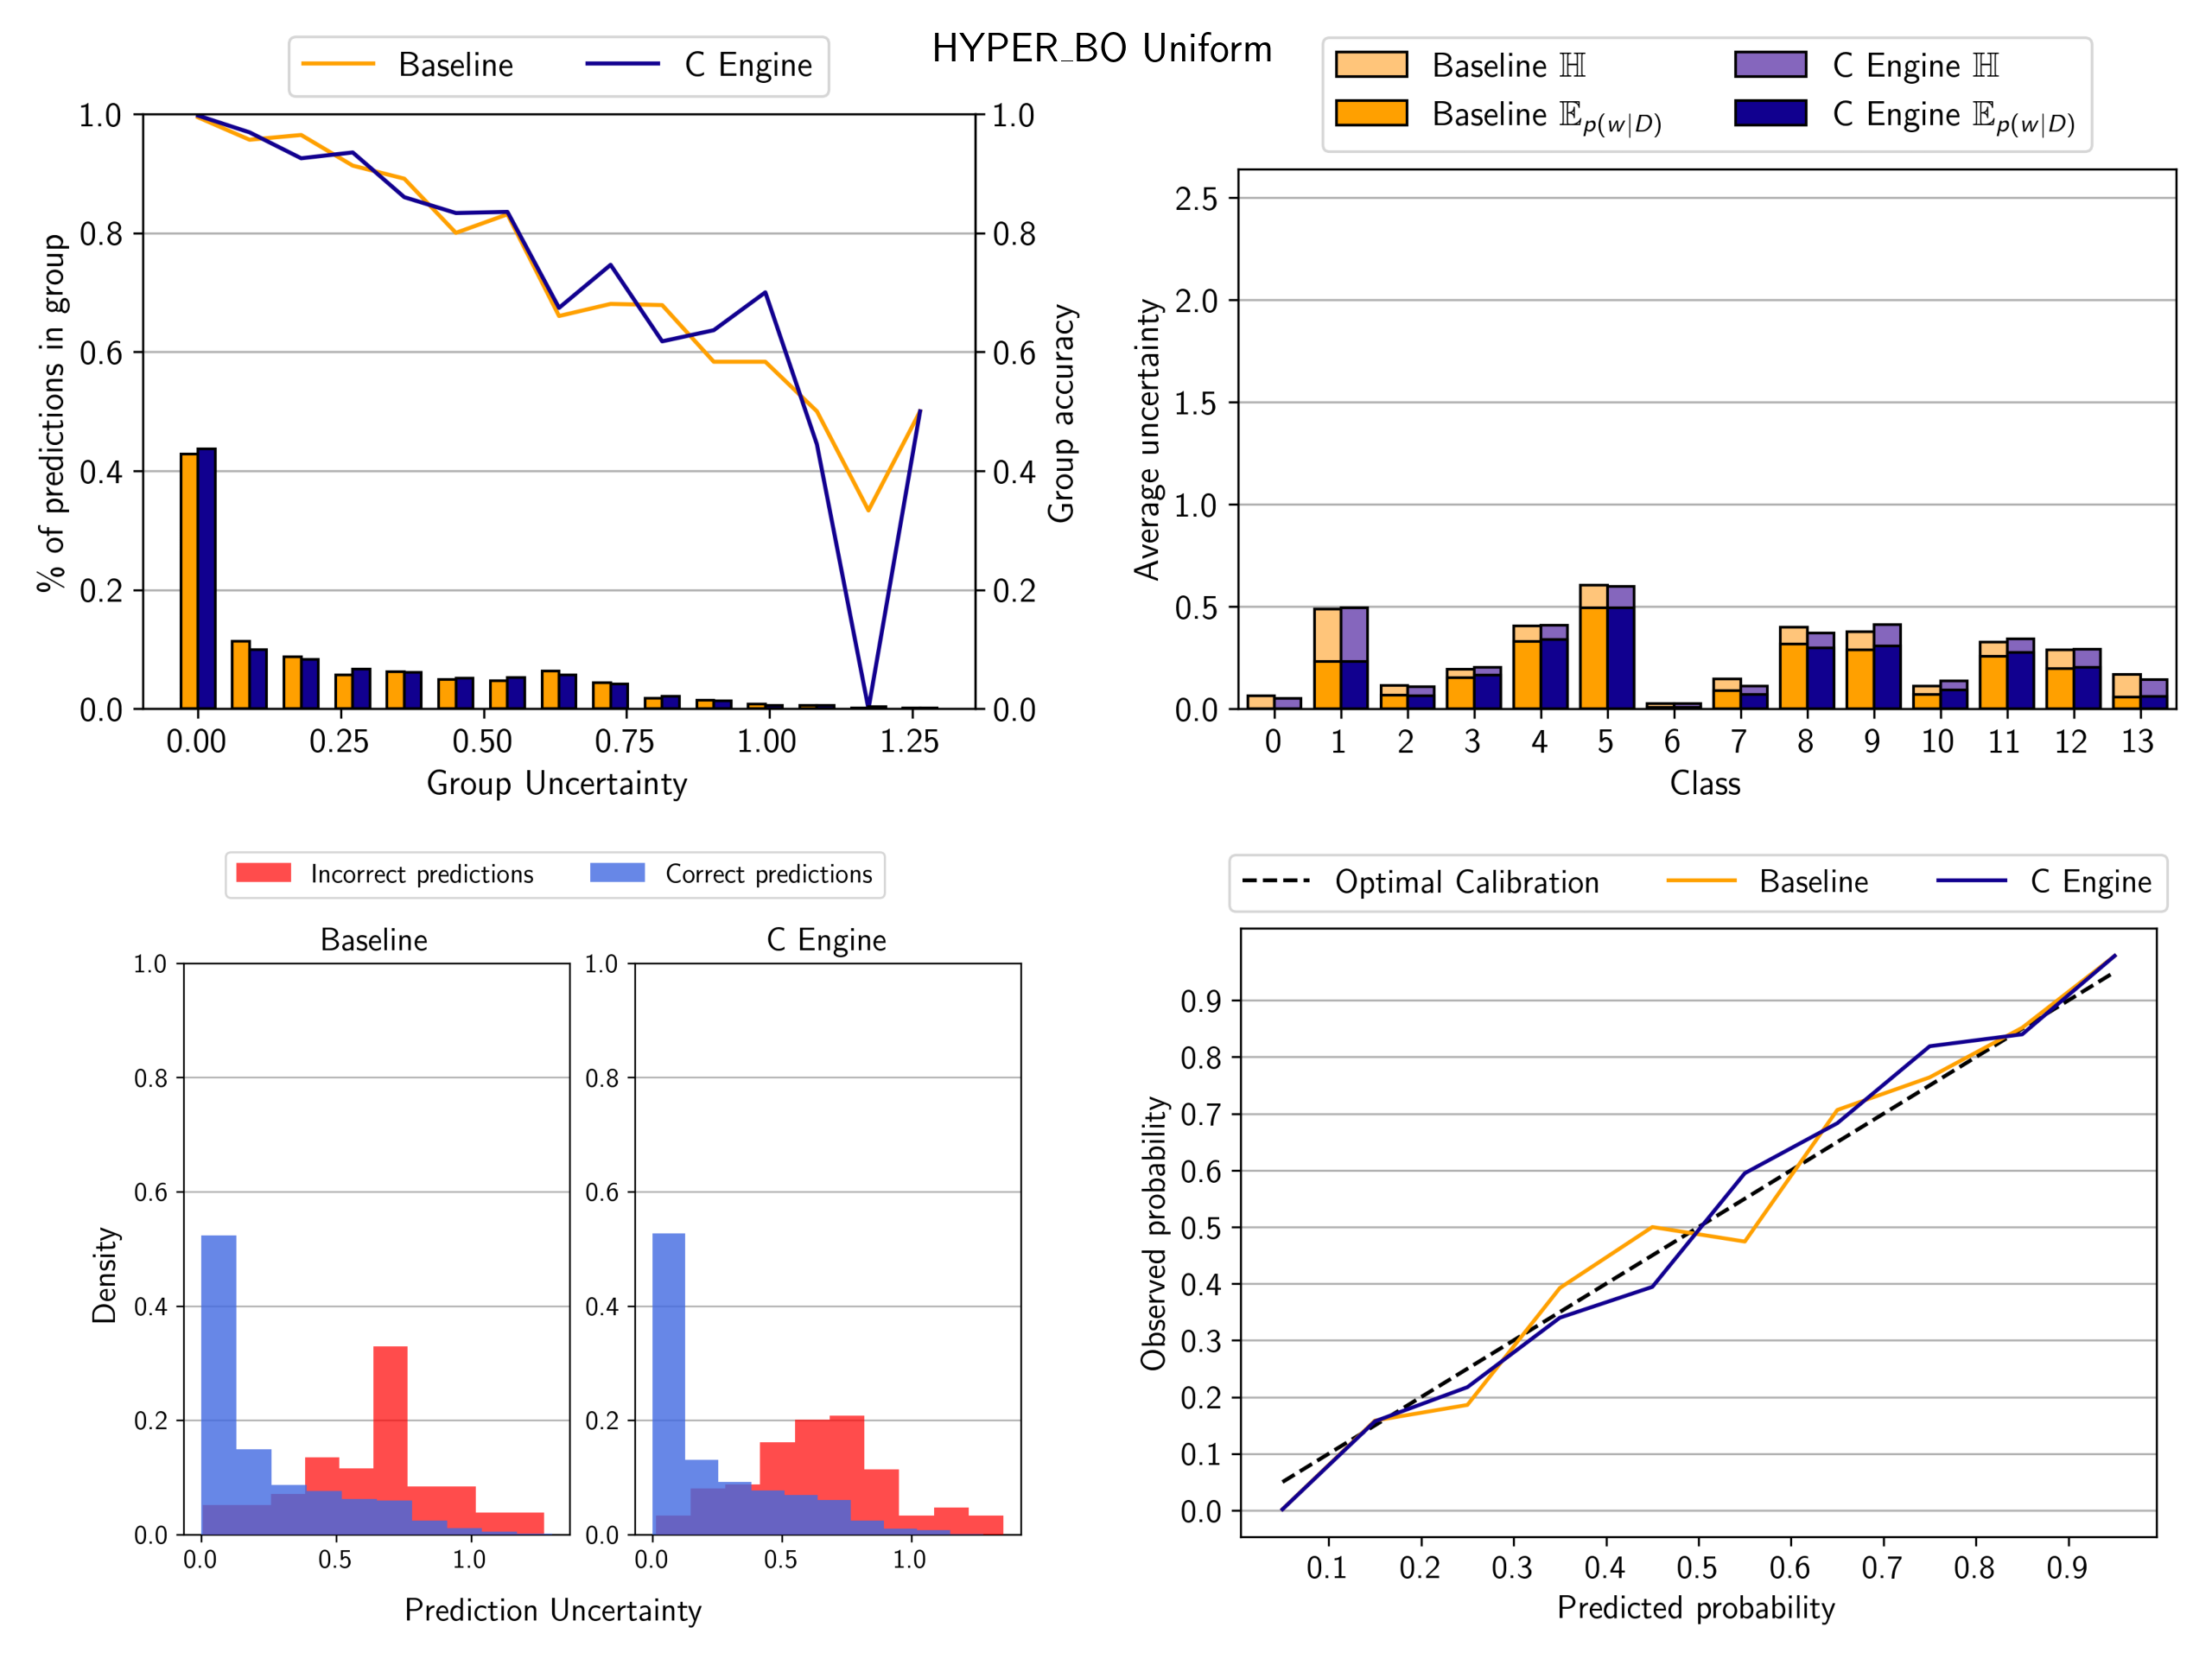
\includegraphics[width=0.9\textwidth]{root/Imagenes/anexo/Uniform-HYPER_BO-mosaic.png}
    \caption{Predicciones del conjunto de prueba de píxeles hiperespectrales BO.}
    \label{fig:anx-Uniform-HYPER_BO}
\end{figure}


\begin{figure}[ht]
    \centering
    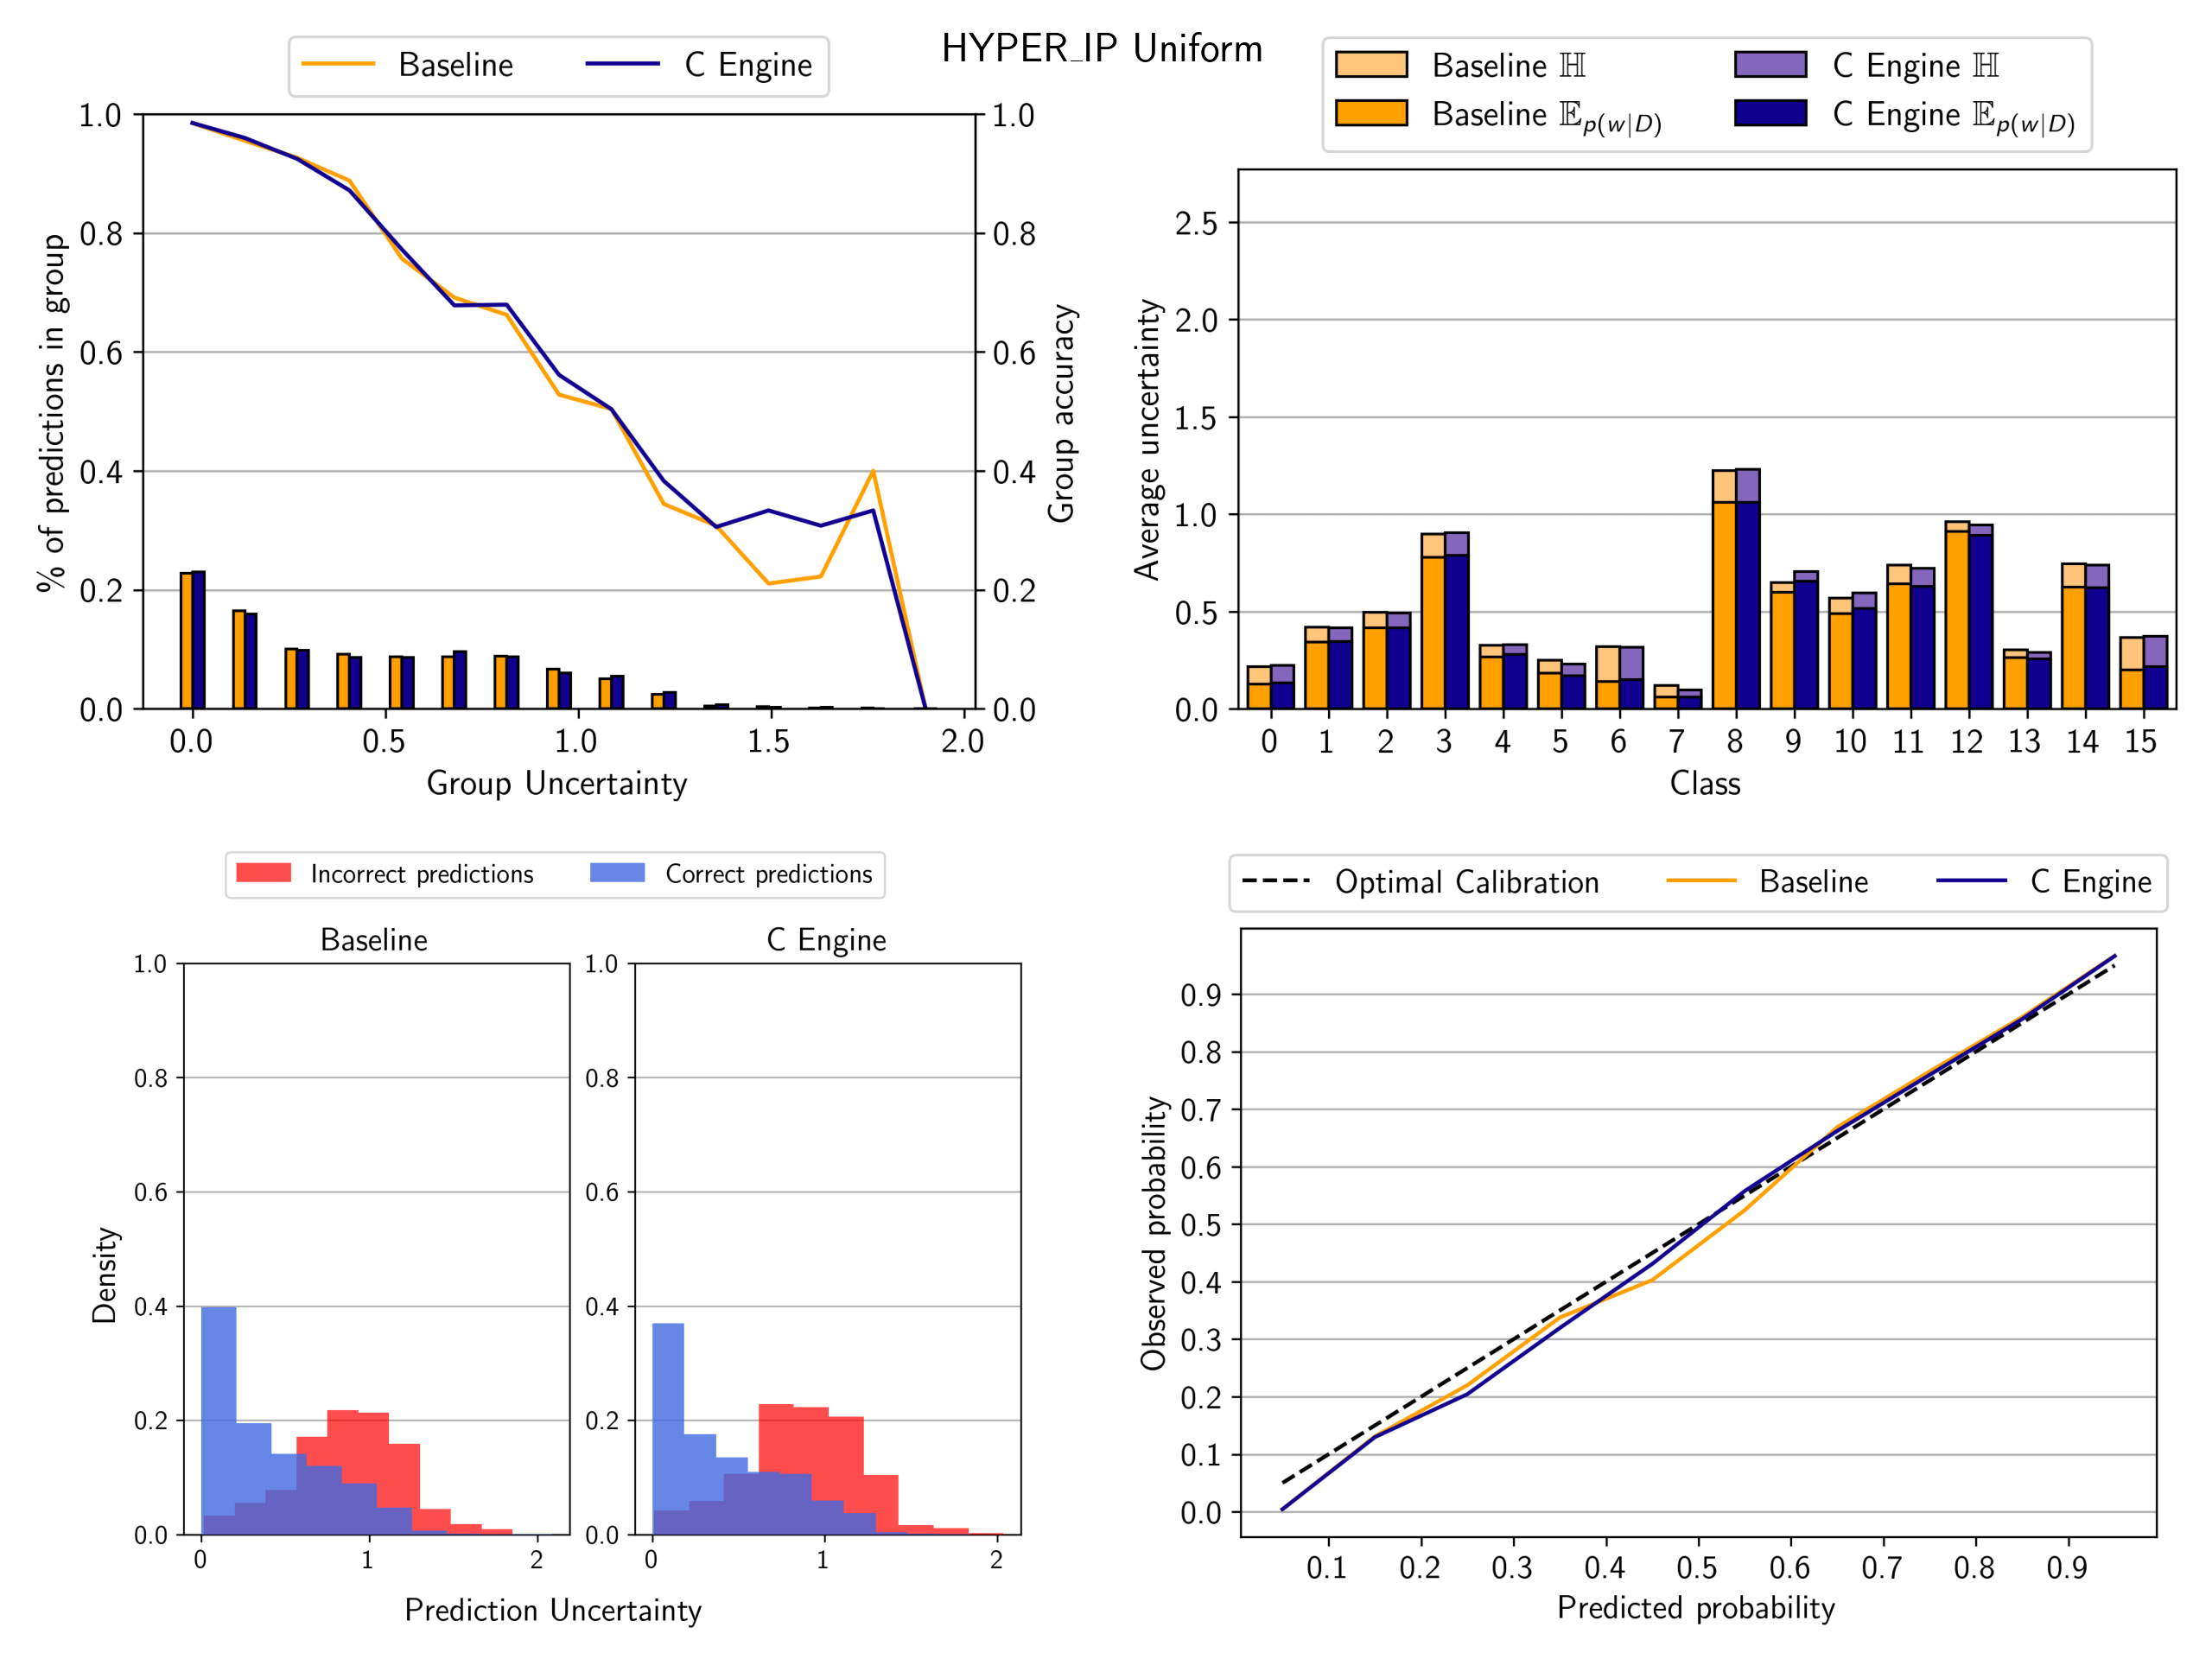
\includegraphics[width=0.9\textwidth]{root/Imagenes/anexo/Uniform-HYPER_IP-mosaic.png}
    \caption{Predicciones del conjunto de prueba de píxeles hiperespectrales IP.}
    \label{fig:anx-Uniform-HYPER_IP}
\end{figure}


\begin{figure}[ht]
    \centering
    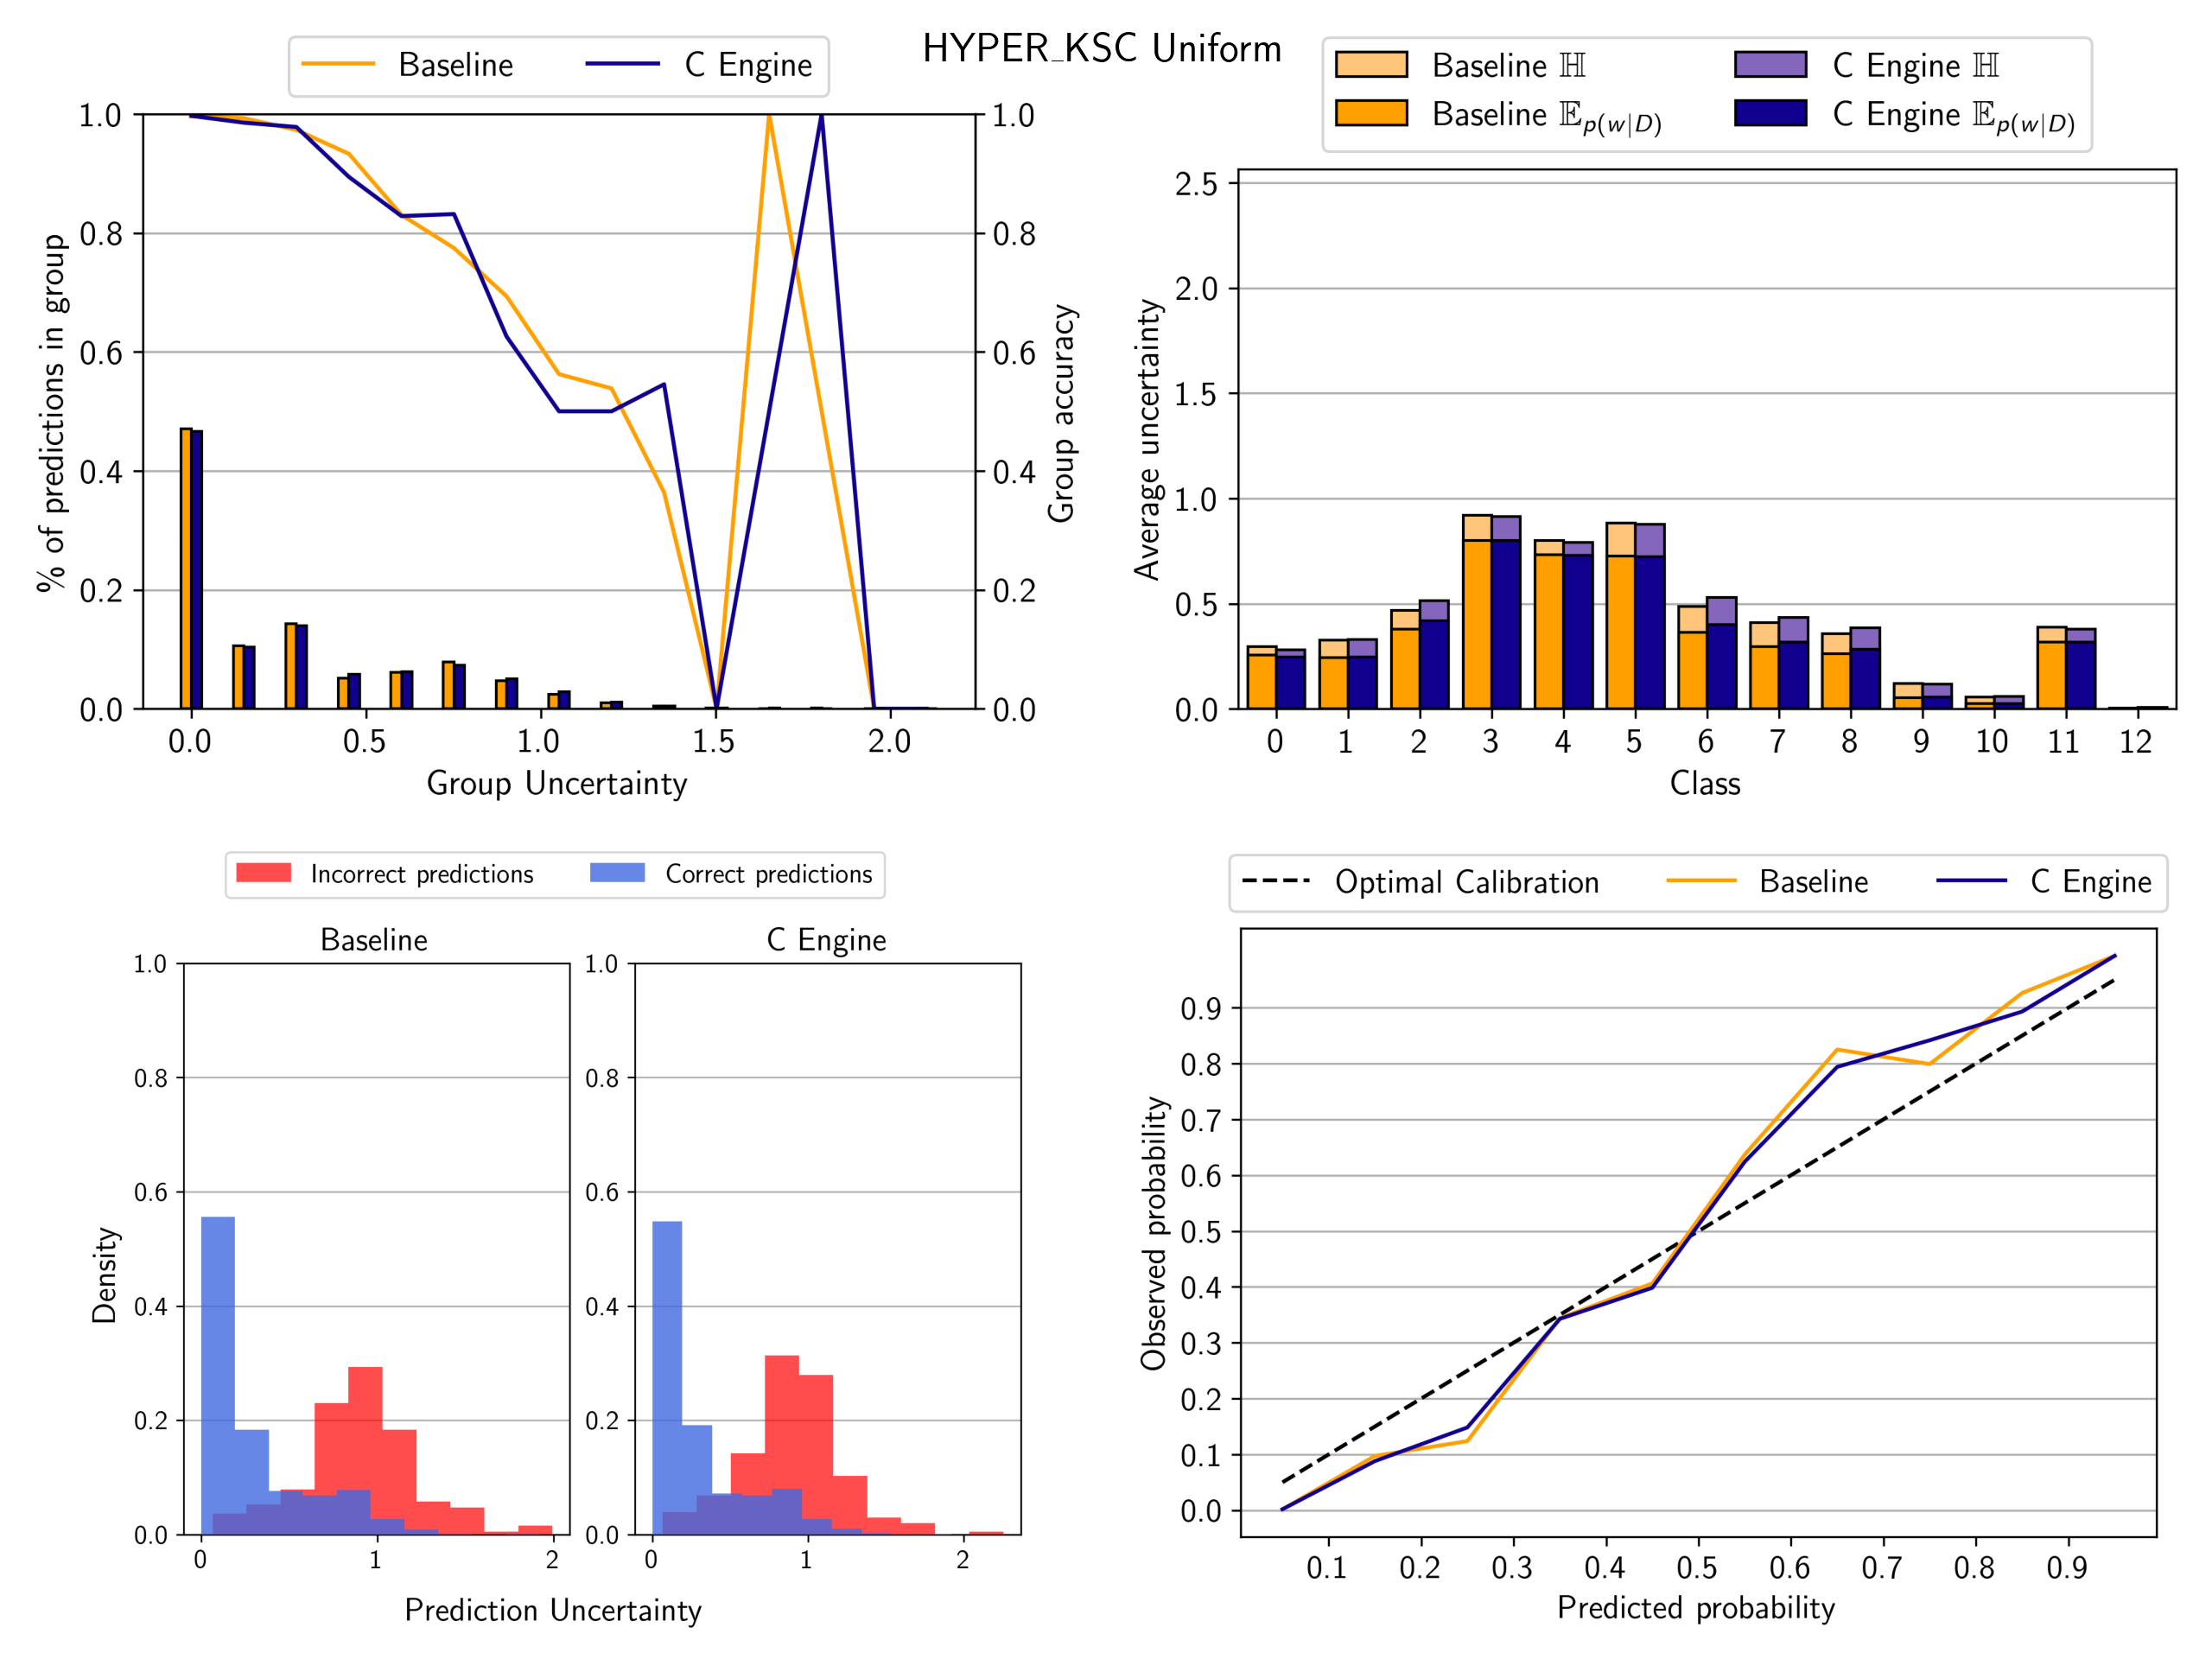
\includegraphics[width=0.9\textwidth]{root/Imagenes/anexo/Uniform-HYPER_KSC-mosaic.png}
    \caption{Predicciones del conjunto de prueba de píxeles hiperespectrales KSC.}
    \label{fig:anx-Uniform-HYPER_KSC}
\end{figure}


\begin{figure}[ht]
    \centering
    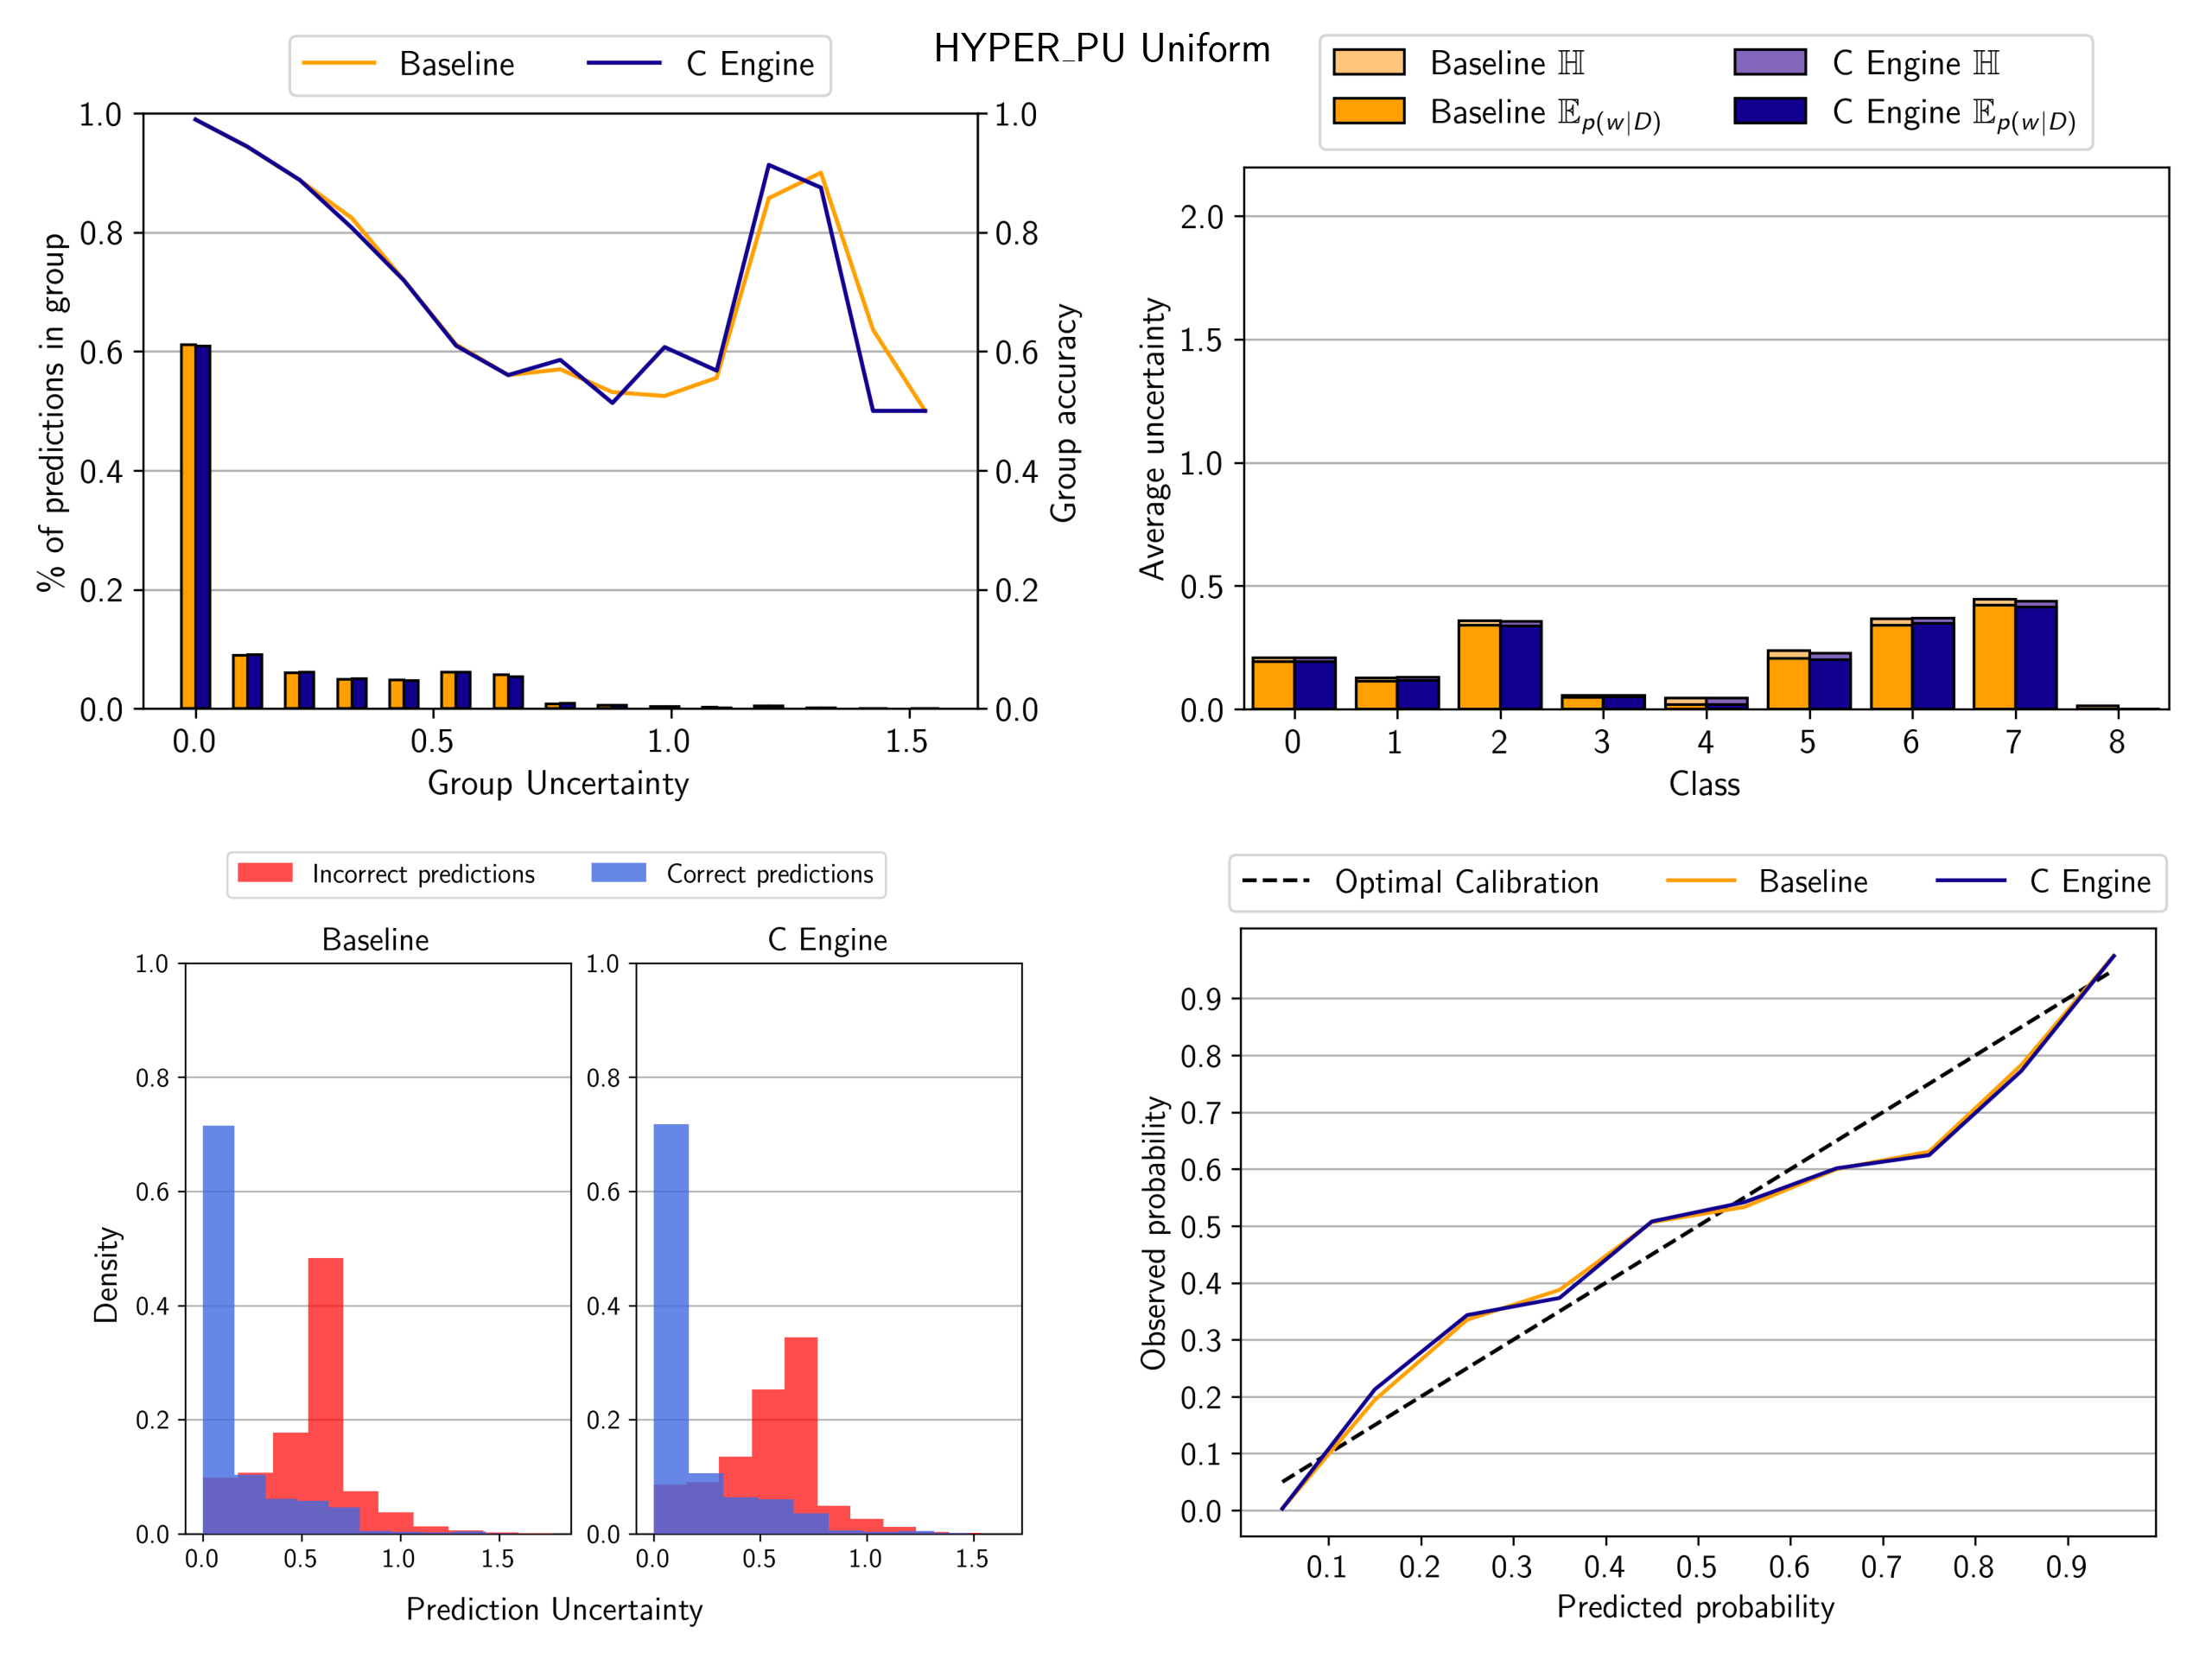
\includegraphics[width=0.9\textwidth]{root/Imagenes/anexo/Uniform-HYPER_PU-mosaic.png}
    \caption{Predicciones del conjunto de prueba de píxeles hiperespectrales PU.}
    \label{fig:anx-Uniform-HYPER_PU}
\end{figure}


\begin{figure}[ht]
    \centering
    \includegraphics[width=0.9\textwidth]{root/Imagenes/anexo/Uniform-HYPER_SV-mosaic.png}
    \caption{Predicciones del conjunto de prueba de píxeles hiperespectrales SV.}
    \label{fig:anx-Uniform-HYPER_SV}
\end{figure}


\begin{figure}[ht]
    \centering
    \includegraphics[width=0.9\textwidth]{root/Imagenes/anexo/Uniform-LENET_MNIST-mosaic.png}
    \caption{Predicciones del modelo LENET con el conjunto de datos MNIST.}
    \label{fig:anx-Uniform-LENET_MNIST}
\end{figure}


\begin{figure}[ht]
    \centering
    \includegraphics[width=0.9\textwidth]{root/Imagenes/anexo/Uniform-LENET_CIFAR-mosaic.png}
    \caption{Predicciones del modelo LENET con el conjunto de datos CIFAR-10.}
    \label{fig:anx-Uniform-LENET_CIFAR}
\end{figure}


\begin{figure}[ht]
    \centering
    \includegraphics[width=0.9\textwidth]{root/Imagenes/anexo/Uniform-B2N2_MNIST-mosaic.png}
    \caption{Predicciones del modelo B2N2 con el conjunto de datos MNIST.}
    \label{fig:anx-Uniform-B2N2_MNIST}
\end{figure}


\begin{figure}[ht]
    \centering
    \includegraphics[width=0.9\textwidth]{root/Imagenes/anexo/Uniform-B2N2_CIFAR-mosaic.png}
    \caption{Predicciones del modelo B2N2 con el conjunto de datos CIFAR-10.}
    \label{fig:anx-Uniform-B2N2_CIFAR}
\end{figure}



%%%%%%%%%%%%%%%%%%%%%%%%%%%%%%%%%%%%%%%%%%%%%%%%%%%%%%%%%%%%%%%%%%%%%%%%%%%%%%%%%%%


\end{document}